\documentclass[oneside,numbers,spanish]{ezthesis}
\usepackage[spanish]{babel}
\usepackage{amssymb}
\usepackage{here}
\usepackage{graphics}
\usepackage{amsmath}
\usepackage{fancyhdr}
\usepackage{longtable}
\usepackage{multirow} %unir renglones
\usepackage[utf8]{inputenc}
\usepackage{multirow}
\usepackage{amsmath}
\usepackage{mathrsfs}
\usepackage{amsfonts}
\usepackage{dsfont}
\usepackage{amssymb}
\usepackage{graphicx}
\usepackage{pdfpages}
\usepackage{multirow}
\usepackage[Conny]{fncychap}
\usepackage{xcolor}
\usepackage{xpatch}
\usepackage{listings}
\usepackage{subfig}
\usepackage{caption}
\usepackage{algorithm}
\usepackage{algpseudocode}
%\usepackage{merriweather} %% Option 'black' gives heavier bold face 
%\usepackage[rm]{roboto}
%\usepackage[T1]{fontenc}
%\usepackage[sfdefault,scaled=.85]{FiraSans}
\usepackage{libertine}
%\usepackage{libertinust1math}
\usepackage{newtxsf}
\usepackage{url}
\usepackage[hidelinks]{hyperref}
\urlstyle{same}
\spanishdecimal{.}
\renewcommand\spanishtablename{Tabla}
\renewcommand\spanishlisttablename{\'{I}ndice de tablas}
\renewcommand{\bibname}{\textbf{Referencias }}
\renewcommand{\tablename}{Tabla}
\renewcommand{\listtablename}{\'{I}ndice de tablas}
\renewcommand{\max}{max}
\renewcommand{\min}{min}
\graphicspath{ {Images/} }
%\definecolor{UNAQ}{HTML}{00335F}
\definecolor{UNAQ}{HTML}{00437e}
\definecolor{mygreen}{rgb}{0,0.6,0}
\definecolor{mygray}{rgb}{0.5,0.5,0.5}
\definecolor{mymauve}{rgb}{0.58,0,0.82}



\newtheorem{definition}{Definici\'{o}n}[section]
\newtheorem{theorem}{Teorema}[section]
\newtheorem{lemma}[theorem]{Lema}
\newtheorem{proposition}[theorem]{Proposici\'{o}n}
\newtheorem{corollary}[theorem]{Corolario}
\newtheorem{comment}[theorem]{Comentario}
\newtheorem{remark}[theorem]{Nota}

%Page header formatting
\pagestyle{fancy}
%Normal pages style
\renewcommand{\headrule}{\hbox to\headwidth{%
  \color{UNAQ}\leaders\hrule height \headrulewidth\hfill}}
\setlength{\headheight}{26pt}
\renewcommand{\headrulewidth}{1.5pt}
\fancyhead[R]{}
\fancyfoot[R]{\thepage}

%Style for chapter headers
\fancypagestyle{plain}{%
  \fancyhf{}
  \fancyhead[L]{
\includegraphics[width=3.5cm]{UNAQBlue.pdf}}
  \fancyfoot[R]{\textbf{\thepage}} 
  \renewcommand{\headrulewidth}{0pt}
  \renewcommand{\footrulewidth}{0pt}
  \setlength{\headheight}{56pt}
}

\fancypagestyle{agrad}{%
  \fancyhf{}
  \fancyhead[L]{}
  \fancyfoot[R]{} 
  \renewcommand{\headrulewidth}{0pt}
  \renewcommand{\footrulewidth}{0pt}
  \setlength{\headheight}{20pt}
}


%Chapter title formatting
\ChNameUpperCase 
\ChTitleUpperCase 
\ChNameVar{\centering\Huge\rm\bfseries\color{black}}
\ChNumVar{\Huge\color{black}} 
%\ChRuleWidth{1pt}
%\ChRuleWidth{0.1px} 
\ChTitleVar{\centering\Huge\rm\color{black}}

\xpatchcmd\DOCH
  {\mghrulefill}{\color{UNAQ}\mghrulefill}
  {}{\PatchFailed}
\xpatchcmd\DOTI
  {\mghrulefill}{\color{UNAQ}\mghrulefill}
  {}{\PatchFailed}
\xpatchcmd\DOTIS
  {\mghrulefill}{\color{UNAQ}\mghrulefill}
  {}{\PatchFailed}

\usepackage{listings}
\lstset{ %
language=bash,                % choose the language of the code
basicstyle=\footnotesize,       % the size of the fonts that are used for the code
%numbers=left,                   % where to put the line-numbers
%numberstyle=\footnotesize,      % the size of the fonts that are used for the line-numbers
stepnumber=1,                   % the step between two line-numbers. If it is 1 each line will be numbered
numbersep=5pt,                  % how far the line-numbers are from the code
backgroundcolor=\color{white},  % choose the background color. You must add \usepackage{color}
showspaces=false,               % show spaces adding particular underscores
showstringspaces=false,         % underline spaces within strings
showtabs=false,                 % show tabs within strings adding particular underscores
%frame=single,           % adds a frame around the code
tabsize=2,          % sets default tabsize to 2 spaces
captionpos=b,           % sets the caption-position to bottom
breaklines=true,        % sets automatic line breaking
breakatwhitespace=false,    % sets if automatic breaks should only happen at whitespace
escapeinside={\%*}{*)},          % if you want to add a comment within your code
commentstyle=\color{mygreen},    % comment style
keywordstyle=\color{blue},       % keyword style
numberstyle=\tiny\color{mygray},
stringstyle=\color{mymauve}
}


%\hyperlinking
\begin{document}




\includepdf[pages=1-1]{PORTADA.pdf}
%\chapter{Conny}



\chapter*{Agradecimientos}
\thispagestyle{agrad}

\textit{\textbf{\large{A mis padres,}}}

que sin ellos no sería quien soy y no estaría donde estoy; los quiero. Les dedico el esfuerzo, la escritura y la propiedad intelectual de este trabajo.

\textit{\textbf{Mamá}}. 

Lety, gracias por ser la persona más bondadosa que he conocido, por apoyarme incondicionalmente y por motivarme a alcanzar mis metas.

\textit{\textbf{Papá}}. 

Lalo, te agradezco por haberme ayudado a formar carácter, por recordarme que siempre debo de creer en mi persona y por todo el apoyo que siempre me has dado.


\textit{\textbf{\large{A mis hermanas,}}}

Saira y Frida, que hacen que la vida tenga sentido, orden y dirección para mi persona.

%Para mi mamá, que me dio la vida, y mi gato, que dio las ganas de vivirla



\chapter*{Resumen}
En este trabajo se integra un conjunto de software de código libre con el objetivo de proponer e implementar un ambiente de simulación para software in the loop, que permita la validación de un sistema propio para la misión de vuelo de un quadrotor; el sistema en cuestión se encuentra integrado por un lado, por un algoritmo de visión por computadora, que cumple con la función de detectar un tipo de compuerta especial que utilizado en competencias de drones autónomos para delimitar un circuito de vuelo, y por otro lado, por un algoritmo de seguimiento de trayectoria basado en waypoints, en donde un programa desarrollado desde cero, se comunica con el firmware de un piloto automático simulado, de tal forma que se envían comandos de vuelo específicos para que el dron sea capaz de volar a través de una serie de compuertas que definen la trayectoria a seguir.

Como se mencionó anteriormente, el sistema de misión de vuelo propuesto está conformado por una serie de aplicaciones y paquetes, entre los cuales se tienen los siguientes:

\textbf{OpenCV}: una paquetería robusta para aplicaciones de visión artificial, con ella se implementó la detección de compuertas

\textbf{PymavLink}: una librería que cuenta con una API basada en MAVLink, con la cual se implementó el seguimiento de trayectoria del dron

\textbf{Gazebo}: un ambiente de simulación para robots, en donde se elaboró el circuito de vuelo 

\textbf{ArduPilot}: un firmware para pilotos automáticos que ofrece herramientas para realizar simulación de software in the loop.

\textbf{ROS 2}: la nueva versión del framework de desarrollo de aplicaciones de robótica; parte esencial para la integración de los algoritmos.

\textbf{GNU/Linux}:  el sistema operativo en donde se desarrolló el proyecto en su conjunto.


Por último, se documenta con gran detalle el proceso de integración de todas las herramientas de software utilizadas, así como el comportamiento final del sistema propuesto.












\chapter*{Glosario}

\textbf{  \normalsize Terminología}
\begin{description}
  \item[\textbf{Algoritmo:}] conjunto finito y ordenado de instrucciones que representan la solución a un problema.
  \item[\textbf{Aprendizaje profundo:}] del inglés '\textit{Deep Learning}', es una subárea de la inteligencia artificial, en donde el modelo de aprendizaje se basa en una gran conjunto de capas (de entrada, salidas y ocultas) compuestas por redes neuronales artificiales. Cada capa se especializa una tarea de predicción específica, de tal forma que una máquina es capaz de aprender por sí misma, sin necesidad de intervención humana.
  \item[\textbf{Arquitectura:}] dentro del campo de estudio de la inteligencia artificial, se refiere a las conexiones o el patrón de diseño de una red neuronal artificial.
  \item[\textbf{Código abierto:}] también conocido como \textit{software libre}, es un modelo de desarrollo de software que se fundamenta en la colaboración abierta, en donde cualquier usuario tiene la liberta de ejecutar, copiar, distribuir, modificar y contribuir a la mejora del software. 
  \item[\textbf{Comando de vuelo:}] dentro del contexto del firmware para pilotos automáticos, se refiere a instrucciones de alto nivel para que el piloto automático lleve a la aeronave a un estado deseado, dígase actitud, rumbo, etc.
  \item[\textbf{Convolución:}] operador matemático que representa la integral del producto de dos funciones, en donde una de las señales se encuentra trasladada e invertida. 
  \item[\textbf{Entrenamiento:}] en el campo de estudio de la inteligencia artificial, se refiere al conjunto de métodos a partir de los cuales una máquina es capaz de aprender.
  \item[\textbf{Espacio de color:}] también conocido como \textit{modelo de color}, se refiere al modelo matemático utilizado para describir los distintos sistemas mediante los cuales se pueden representar los colores, a partir de arreglos de 3 o 4 parámetros, generalmente.
  \item[\textbf{Firmware:}] es el software base que viene incluido en los dispositivos electrónicos o hardware, y se encarga de asegurar un funcionamiento básico correcto. También es conocido como \textit{soporte lógico inalterable}.
  \item[\textbf{Fotograma:}] cada una de las imágenes fijas, que en su conjunto forman una imagen en movimiento o video.
  \item[\textbf{Framework:}] en español \textit{entorno de trabajo}, es una estructura que integra tecnologías, estándares y módulos de software que sirve como base para el desarrollo software.
  \item[\textbf{Hardware:}] corresponde a los recursos físicos que componen o integran un equipo de cómputo o dispositivo lógico.
  \item[\textbf{Hardware in the loop:}] paradigma de simulación para la validación de sistemas embebidos en donde la planta que se desea controlar se simula a partir de un modelo matemático, mientras que el sistema de control es físico e interactúa de forma directa con la simulación de la planta.
  \item[\textbf{Histograma de color:}] es la cuantificación de la distribución de color en una imagen, generalmente se representa con una gráfica en donde se observa la frecuencia de pixeles del mismo color.
  \item[\textbf{Interfaz de programación de aplicación:}] del inglés \textit{Application} \textit{Programming} \textit{Interface}; se trata de un conjunto de definiciones y protocolos que permiten la comunicación o integración entre diferentes aplicaciones de software.
  \item[\textbf{Librería:}] también conocidas como \textit{bibliotecas}, es un conjunto de módulos o métodos funcionales de software, que fueron codificados para ofrecer una funcionalidad especifica y bien definida.
  \item[\textbf{Machine learning:}] conocido en español como \textit{aprendizaje automático}, es una subárea del campo de la inteligencia artificial en donde se implementa modelo matemático para que un sistema sea capaz de aprender a partir del procesamiento de datos sin la necesidad de especificar una programación explicita.
  \item[\textbf{Máquina de estados:}] es un modelo que describe el comportamiento de un sistema a partir de una serie de estados finitos, en donde la transición entre cada uno depende de la entrada actual del proceso y la o las entradas anteriores.
  \item[\textbf{Matiz:}] en el modelo de color HSV, corresponde a un ángulo dentro del rango de 0 a 360 grados, en donde cada grado está asociado a una tonalidad de color en específico.
  \item[\textbf{Multiplataforma:}] dicho de una aplicación de software que se encuentra disponible para su ejecución en distintos sistemas operativos o sistemas.
  \item[\textbf{Odometría:}] es el área que se encarga del estudio de la estimación de posición de cualquier tipo de vehículo durante su navegación.
  \item[\textbf{Quadrotor:}] aeronave de despegue y aterrizaje vertical que es levantado y propulsado por cuatro rotores.
  \item[\textbf{Rapid control prototyping:}] paradigma de validación de sistemas en donde un prototipo físico de la planta interactúa con un modelo matemático o simulación del controlador de esta.
  \item[\textbf{Red neuronal artificial:}] es un sistema informático que busca emular las redes neuronales biológicas a partir de funciones u operaciones matemáticas.
  \item[\textbf{Saturación:}] en el modelo de color HSV, se refiere a la pureza del matiz, representa la distancia al eje de brillo negro-blanco.
  \item[\textbf{Script:}]  es una secuencia de comandos o instrucciones que conforman un programa informático relativamente simple.
  \item[\textbf{Segmentación:}] dentro del campo del procesamiento de imágenes, se refiere al proceso de dividir una imagen en distintas regiones con atributos similares, logrando hacer una distinción clara entre la información de interés y la información no relevante para el análisis.
  \item[\textbf{Sistema operativo:}] es software encargado de gestionar los recursos de hardware de un sistema informático.
  \item[\textbf{Software in the loop:}] paradigma de validación de sistemas en donde la planta y el sistema de control se representan mediante un modelo matemático e interactuar dentro de una simulación.
  \item[\textbf{Terminal de comandos:}] es una interfaz que le permite al usuario interactuar con un sistema de cómputo de forma explícita a base de un conjunto de instrucciones o comandos bien definidos.
  \item[\textbf{Validación:}] en el ámbito del la gestión y desarrollo de proyectos de software se refiere a la evaluación del producto para determinar si cumple con las expectativas y requerimientos definidos por el cliente.
  \item[\textbf{Valor:}] dentro del modelo de color HSV, se refiere al brillo del matiz y representa un desplazamiento vertical en el eje blanco-negro.
  \item[\textbf{Waypoint:}] es un punto de referencia intermedio que conforma una trayectoria o una ruta para el desplazamiento de algún vehículo.
                        
\end{description}
\clearpage

\textbf{Abreviaturas y acr\'onimos}

\begin{description}
\item[API] Application Programming Interface.
\item[HIL] Hardware in the Loop.
\item[SIL] Software in the Loop.
\item[RCP] Rapid Control Prototyping.
\item[RNA] Red Neuronal Artificial.
\item[ML] Machine Learning.
\item[DL] Deep Learning.     
\item[ROS] Robot Operating System 
\end{description}




\tableofcontents
\listoffigures
\listoftables

\chapter{Introducción}

\section{Antecedente históricos}
En diciembre de 1903, Orville Wright realizó el primer vuelo tripulado en la historia de la humanidad; no tuvo que pasar mucho tiempo para que el concepto de vehículo aéreo no tripulado tuviera un auge dentro de la comunidad científica y militar enfocada a la aviación.

Siendo estrictamente correctos, si se toma en consideración los vehículos capaces de generar sustentación y/o que cuentan con un medio para su control, se puede decir que el primer UAV de la historia, fue diseñado por el inglés Douglas Archibald, al fijar un anemómetro en la cuerda de un cometa, con lo cual fue capaz de medir  la velocidad del viento a una altura de aproximadamente 1200 ft. Más tarde, en 1887, Archibald colocó cámaras en otra cometa, con lo cual desarrolló el primer UAV de reconocimiento, en el mundo.

Hablando específicamente de quadrotores, en 1907, Louis Breguet, un pionero francés de la aviación, junto con su hermano Jacques y su profesor Charles Richet, hicieron una demostración del diseño de un giroplano de 4 rotores. Este prototipo contaba con un motor de 30 caballos de fuerza que alimentaba los 4 rotores, cada uno de los cuales tenía 4 propelas y lograba elevarse hasta un máximo de 0.6 m.

Por otro lado, Etienne Oehmichen, un ingeniero francés, fue el primero en experimentar con diseños de aeronaves de ala rotativa. En 1920, construyó y probó 6 diseños, el segundo de ellos tenía 4 motores y 8 propelas; el cuerpo de esta aeronave estaba hecho de tubos de acero y tenía 4 extremidades, en las cuales se alojaban cada uno de sus rotores con 2 propelas cada uno. En su momento, este diseño destacaba en su estabilidad y controlabilidad, y para la mitad de 1920 ya había realizado más de mil vuelos de prueba. En 1924 estableció un récord mundial al volar una distancia horizontal de 360 m.

Después, en 1922 el Dr. George de Bothezt e Ivan Jerome desarrollaron una aeronave con una estructura en forma de equis y rotores de 6 propelas en sus extremidades. Para 1923 habían realizado hasta 100 vuelos de prueba con una altura máxima de 5 m; sin embargo, este diseño era muy complejo y rígido, dificultando su movimiento lateral y suponiendo una  carga de trabajo, para alimentar la maquinaria, demasiado alta para el piloto.

Además, en 1956 se desarrolló el Convertawings Model A, el cual fue pensado para formar parte de una línea de quadrotores grandes para uso civil y militar. Este prototipo contaba con dos motores, que controlan el giro de dos rotores, cada uno, a partir de lo anterior, el control de la aeronave se lograba al variar el empuje proporcionado por los rotores.


%\section{Motivación}



\section{Objetivos}
\subsection{Objetivo general}

Proponer e implementar en simulación un algoritmo de detección de compuertas rectangulares mediante visión artificial para la definición y control de trayectoria de un cuadricóptero autónomo virtual.  


\subsection{Objetivo específicos}

\begin{itemize}
    \item Diseñar un algoritmo de visión artificial capaz de identificar compuertas rectangulares 
    \item Diseñar un algoritmo de gestión de trayectorias de vuelo para un cuadricóptero autónomo 
    \item Diseñar un ambiente de simulación en 3D de un circuito de vuelo basado en una carrera de cuadricópteros autónomos. 
    \item Implementar un ambiente de Software in The Loop utilizando los algoritmos y el ambiente de simulación diseñados para verificar su comportamiento en conjunto 
\end{itemize}

\section{Justificación}
Lejos de ser un atractivo visual y un espectáculo con fines de entretenimiento, las competencias de drones autónomos representan el estado del arte de la robótica aplicada a vehículos con sistemas de navegación autónoma.
Lo anterior se debe a que la robótica siempre se ha enfocado a la automatización de los sistemas; es decir, que los robots sean capaces de realizar tareas o recorridos sin necesidad de intervención humana, para esta última parte, se necesita de algoritmos de percepción y navegación, con los cuales los vehículos puedan ubicarse en el espacio a partir de su sistema de sensores con el que cuentan (tales como tecnología a base de láseres, cámaras estereoscópicas, tecnología ultrasónica, etc.) para que después sea capaz de trazar una trayectoria o seguir una ruta previamente definida.   
Lo anterior ha adquirido una robustez bastante significativa en los últimos años, pues existe una gran cantidad de esfuerzos y colaboraciones dedicadas al desarrollo de los mismos, incluso, se han organizado eventos y competencias con el fin de estimular y potenciar el desarrollo de este tipo de sistemas; tal es el caso de la International Conference on Intelligent Robots and systems (IROS) y AlphaPilot, dos eventos de gran magnitud, creados con el objetivo de tratar, demostrar y fomentar los avances que se tienen en el área.

Por otro lado, la implementación de un sistema robótico autónomo no es una tarea sencilla, y debido a la poca competencia en el mercado también adquiere un costo elevado. 
Para que un robot sea capaz de percibir el ambiente a su alrededor y desplazarse por el mismo, es necesario implementar un sistema de software capaz de coordinar la adquisición de datos proveídos por los sensores y el conjunto de actuadores que permiten que el sistema se desplace. Muchas de las soluciones desarrolladas para afrontar este desafío son privadas y no sé comparte con el público en general, además, algoritmos como el filtro de Kalman o un control PID son ampliamente utilizados en este tipo de sistemas, por lo que existe una posibilidad bastante alta de que todas estas soluciones implementen los mismos algoritmos, lo cual conlleva un desperdicio de tiempo y esfuerzo, sin mencionar que la calidad y eficiencia de cada implementación puede variar bastante.
Debido a lo anterior, soluciones de código abierto como ROS (Robot Operating System; un framework de comunicaciones para el manejo y coordinación de procesos en sistemas robóticos), pueden representar el inicio de la implementación de un estándar en el área, pues al ser de software libre permiten que toda la comunidad utilice, mejore e inspeccione los algoritmos ya implementados.

Además, la realización de pruebas con el sistema físico, para verificar y validar los algoritmos desarrollados, representa un costo muy alto en la mayoría de sistemas con los que se trabaja en el área, por lo que también es necesario disponer de algún tipo de simulador que permita realizar las pruebas sin necesidad de utilizar el prototipo físico con el que se trabajará. Existen diferentes paradigmas de simulación en los que se puede simular la planta mediante software, tales como Hardware in the loop (HIL) y software in the loop (SIL). Ambos paradigmas representan una solución al problema planteado, proveyendo resultados muy cercanos a la realidad y con una arquitectura flexible, que permite realizar una gran cantidad de pruebas o incluso entrenar algoritmos relacionados con inteligencia artificial o redes neuronales, una vez más, sin depender del sistema físico. 

A partir de todo lo anterior, en este trabajo se propone el diseño y la simulación de un algoritmo de visión por computadora para la detección de compuertas rectangulares, similares a aquellas utilizadas en las competencias de drones autónomos, para definir la trayectoria de vuelo de un dron autónomo con el fin de que sea capaz de completar un circuito definido.  El entrenamiento e implementación se realizan dentro de un framework de simulación de SIL, y la gestión y comunicación entre procesos se implementan a partir de una arquitectura diseñada en ROS2, todo lo anterior bajo el paradigma de código abierto con el fin de aprovechar las ventajas previamente mencionadas y aportar los esquemas de configuración y diseño a la comunidad.

\vfill



%\section{Planteamiento del problema}


%\section{Contribuciones}


\section{Metodología}

En primera instancia, se realiza una revisión bibliográfica intensiva acerca del estado del arte en cuanto a drones guiados por visión artificial, con el objetivo de visualizar las soluciones ya implementadas y conceptualizar la arquitectura necesaria para el sistema, sus componentes, los algoritmos de visión artificial empleados y la configuración necesaria para realizar la integración de todo lo anterior.

Posteriormente, se define el esquema general del proyecto estableciendo el algoritmo de visión artificial a utilizar, el ambiente de simulación, la interfaz de comunicación para la adquisición de datos e imágenes provenientes de la simulación, el modelo de dron a simular y las librerías necesarias para integrar el ambiente de simulación.

Establecido lo anterior, se implementa la arquitectura diseñada para el ambiente de simulación y se realizan vuelos manuales con el modelo de dron definido dentro de un circuito de prueba compuesto por compuertas. A partir de lo anterior, se extraen imágenes de la trayectoria de vuelo del dron por medio de una cámara simulada a bordo del modelo del dron; se utilizan las imágenes recopiladas para el entrenamiento del algoritmo de visión artificial.

Cuando el algoritmo de visión artificial proporciona una identificación adecuada del tipo de compuerta utilizada, se implementa el algoritmo con base en la arquitectura definida. Se realiza la validación del algoritmo en otro circuito de vuelo; a lo largo de la simulación, existe un intercambio de información constante entre la simulación y el algoritmo de visión artificial, la simulación envía imágenes obtenidas durante el vuelo del dron y el algoritmo de visión artificial las analiza, de tal forma que es capaz de identificar el centro de la compuerta más cercana y devuelve comandos de vuelo a la simulación para definir una ruta de vuelo que permita que el dron sea capaz de volar a través de la compuerta identificada y finalizar el circuito de forma autónoma.

Se reportan los resultados obtenidos y las posibles mejoras para el proyecto en su conjunto



\section{Límites y alcances}

\subsection{Alcances}
Se implementa la arquitectura de red neuronal convolucional (RNC) DeepPilot, la cual toma capturas de la única cámara a bordo del drone y predice cuatro comandos de vuelo ($\phi,\theta\psi,h$) como salida. La RNC es entrenada a partir de un dataset proveído por los autores de la arquitectura y que contiene un gran conjunto de imágenes obtenidas a partir de simulación, las cuales están asociadas a ciertos comandos de vuelo.    La arquitectura es evaluada dentro de un entorno de simulación realizado en simulador Gazebo 11, en donde se virtualiza un circuito o pista de obstáculos compuesta por compuertas rectangulares de distintas alturas y color sólido, colocadas en distintas posiciones y orientaciones a lo largo del circuito. Se utiliza ROS2 para coordinar el envío de datos entre la simulación de Gazebo 11 y un nodo propio de ROS2 que contiene el algoritmo y arquitectura de DeepPilot. Además, se documenta de forma detallada la configuración realizada para la creación del ambiente de simulación, especificando la integración entre Gazebo, ROS y Python 3 para la evaluación de la arquitectura de DeepPilot. Por último, el proyecto en su conjunto se distribuye bajo el paradigma de código abierto.

\subsection{Límites}
A diferencia de las contribuciones y proyectos más populares dentro de la comunidad de las carreras de drones autónomos, en donde se utiliza ROS1 y Gazebo en su versión 9, en este proyecto se implementa la última versión estable de ROS2, Foxy, y la versión más actual del simulador Gazebo, al momento de escritura del trabajo, la versión 11. Por lo que es muy posible que algunos plugins tanto de ROS como de Gazebo, no se encuentren disponibles en estas versiones, lo que significa una limitante para la expansión a futuro del proyecto.  Por otro lado, dentro del ambiente de simulación, no se evalúan condiciones de vuelo poco ventajosas como viento en contra, lluvia o cualquier otra condición climática adversa. Además, la complejidad en el arreglo de compuertas para el circuito es baja y se asume que las compuertas se encuentran de forma paralela a la cámara del dron, y  es necesario que siempre exista una compuerta visible después de haber cruzado por otra.


\section{Estructura de la tesis}








\chapter{Estado del Arte}

Las competencias de drones autónomos han adquirido un grado alto de relevancia en la última década, dentro del marco teórico del presente trabajo se describe con profundidad el contexto histórico, así como la motivación y los requerimientos establecidos para dos de las competencias, más significativas, de drones autónomos, el  IROS Autonomous Drone Race y el AlphaPilot AI Drone Innovation Challege. 
En este capítulo se presentan algunas de las soluciones propuestas en estas competencias, al igual que trabajos con enfoques más prácticos o que no se encuentran directamente relacionados con las carreras de drones autónomos.

Dentro de las competencias anteriormente mencionadas, existen dos problemas esenciales a los que se enfrentan los equipos que participan en estos retos, la detección de objetos y la gestión de trayectoria de vuelo a partir de la detección realizada. 
Los circuitos que tiene que completar los drones están compuestos por compuertas de distintas formas y tamaños, y en algunos casos, se adicionan obstáculos dinámicos, los vehículos desarrollados por los participantes tienen que ser capaces de detectar estos objetos haciendo uso exclusivo de los sensores con los que están equipados (cámaras, sensores ultrasónicos, tecnología láser, etc.).

Con base en lo anterior, Cabrera et al.(2019). \cite{cabrera2019gate} desarrollaron un algoritmo para la detección de compuertas en tiempo real basado en aprendizaje profundo. Su implementación se basó en una arquitectura de red neuronal convolucional con una arquitectura base de Single Shot Detector de 7 capas (SSD7\cite{SSD7}). La arquitectura base tiene un diseño optimizado para la detección de objetos, permitiendo un tiempo de entrenamiento reducido y una velocidad de detección alta; esta se modificó de tal forma que se eliminaron las últimas dos capas convoluciones, haciendo posible una detección mucho más rápida que la propuesta base y disminuyendo la complejidad de la red. El entrenamiento de la red se realizó con un total de 3418 imágenes obtenidas a partir de un entorno simulado y entornos reales. 
Además, para observar el desempeño de su implementación compararon su arquitectura con otras propuestas, SSD7, SSD300 y SmallerVGG, en simulaciones y ambientes de exteriores e interiores. Los resultados muestran que su propuesta logra un tiempo de detección promedio más bajo y porcentaje de confianza más alto que las otras arquitecturas. 

Por otro lado, Mellinger y Kumar (2011)\cite{mellinger2011minimum} presentaron un diseño de control y generación de trayectoria de vuelo en ambientes de interiores para un quadrotor. Su implementación es capaz de generar una trayectoria óptima y ángulos para la guiñada del vehículo, en tiempo real, a partir de matrices de rotación para el marco de referencia del vehículo y una secuencia de posiciones en tres dimensiones. La propuesta fue diseñada con el objetivo de que el quadrotor sea capaz de navegar de forma segura a través de corredores angostos, manteniéndose en los límites de velocidad y aceleración. Además, implementaron un control no lineal que asegura el seguimiento de las trayectorias generadas; las propuestas se pusieron a prueba con un prototipo físico  que se hizo volar a través de un circuito construido por aros, los cuales indicaban la trayectoria que el quadrotor debía de seguir.

A demás, Mueller et al.(2013)\cite{mueller2013computationally} diseñaron un algoritmo de bajo consumo computacional para la generación de trayectorias de intersección vuelo de un quadrotor. La implementación tuvo como propósito que el quadrotor fuera capaz de interceptar una pelota en vuelo, con una raqueta montada en su chasis. El algoritmo de generación de trayectoria se usó en un sistema de control predictivo, en donde miles de trayectorias eran generadas y evaluadas por el controlador, y después, la trayectoria más óptima era seleccionada por el algoritmo.  Se destaca el bajo coste computacional pues se utilizó el hardware de una laptop estándar para evaluar cerca de un millón de trayectorias por segundo.

Las propuestas anteriores representan ejemplos de soluciones individuales para cada uno de los problemas mencionados. Sin embargo, existen implementaciones que solucionan ambos problemas en un solo trabajo, y corresponden a aquellas que fueron desarrolladas como propuestas para participar en las competencias.  



\chapter{Marco Teórico}

\section{Competencias de Drones Autónomos}

 
\section{Robot Operating System (ROS)}

De acuerdo con su sitio oficial, ROS (del inglés, Robot Operating System) es un conjunto de herramientas y librerías de software para robótica desarrolladas por Open Robotics bajo el paradigma de software libre u open-source. Este entorno de trabajo destaca por contener algoritmos de última generación y herramientas de desarrollo avanzadas,  que permiten la creación, implementación y reutilización de código para todo tipo de proyectos de robótica.

ROS 1, la primera versión del entorno de trabajo, surgió en 2007 como un ambiente de desarrollo para el PR2 robot, un robot de servicio diseñado para trabajar con personas y creado por la empresa The Willow Garage. Sin embargo, los creadores de ROS buscaban que el entorno de trabajo no se viera limitado a un solo modelo de robot, sino que, pudiera ofrecer herramientas de software para más tipos y modelos de robots, por lo que ROS adquirió varias capas de abstracción mediante la implementación de interfaces para el manejo de mensajes, lo que dio lugar a que el software desarrollado mediante ROS pudiera ser reutilizado en más robots.   

Algunas características que destacan en esta etapa temprana de ROS son:
Gestión de un solo robot
Sin requerimientos de aplicación en tiempo real
Excelente conectividad a la red
Usado principalmente en el ámbito académico y de investigación

Hoy en día, ROS es utilizado en una amplia gama de robots, desde robots con ruedas y con forma humanoide, hasta brazos industriales, vehículos aéreos y mucho más. Sin embargo, ha pasado bastante tiempo desde el lanzamiento de la primera versión de ROS, y las necesidades y estándares de la industria han cambiado al igual que el paradigma y la filosofía detrás del desarrollo de ROS.
   
A partir de lo anterior, en 2014 una nueva versión de ROS con un enfoque y estructura distinta es anunciada por Open Robotics.  ROS 2 surge como un completo rediseño para lo que había sido el entorno de trabajo hasta entonces, con esta reestructuración se busca cubrir necesidades y funcionalidades que no habían sido consideradas con  ROS1, pero que habían sido exigidas por la comunidad y la industria. Lo anterior dio lugar al desarrollo de un nuevo conjunto de paquetes 

\section{Visión Artificial}

\section{Software in The Loop}

\section{Gazebo}


\chapter{Proceso de configuración y ambiente de simulación}

En este capítulo se presentan los resultados obtenidos; además, se documenta de forma detallada el procedimiento realizado para configurar cada uno del software utilizado, lo anterior debido a que este trabajo también busca funcionar como una guía estructurada que permita la réplica del la implementación desarrollada.

\section{Configuración del Framework de SIL}
La implementación del trabajo se realizó en una computadora portátil modelo \textit{Acer Aspire E5-575}. A continuación se anexan las características físicas más relevantes del hardware utilizado.

\begin{table}
    \centering
    \begin{tabular}{ll}
        \hline
        Parámetro & Descripción\\
        \hline
        \hline
        Procesador & Intel Core i3-7100U; Dual-core 2.40 GHz\\
        Memoria RAM & 12 GB DDR4\\
        Disco duro & 1 TB Toshiba HDD\\
        Coprocesador de gráficos & Intel HD Graphics 620\\
        \hline
        \hline
    \end{tabular}
    \caption{Características técnicas de la laptop Aspire E5-575}
    \label{tab:specs}
\end{table}

La figura \ref{fig:req} muestra con más detalle las características de hardware y software correspondientes a la computadora donde se llevó a cabo el proyecto. 

\begin{figure}[ht]
    \centering
    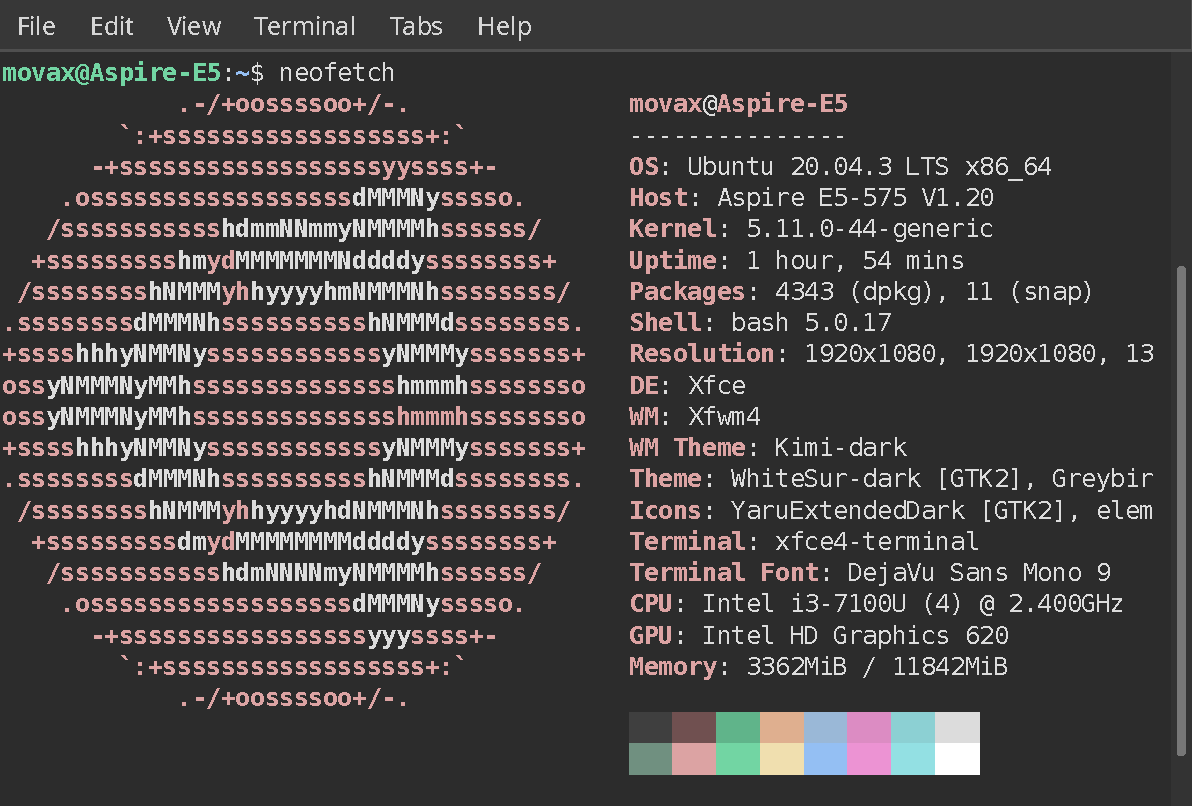
\includegraphics[width=0.6\textwidth]{System_req.pdf}
    \caption{Características del sistema en donde se desarrolló el proyecto}
    \label{fig:req}
\end{figure}

Con respecto al software, se trabajó con las versiones más recientes y técnicamente compatibles del software que integra el sistema. Para el ambiente de simulación se utilizó \textit{Gazebo 11} en conjunto con \textit{ArduPilot} y el modelo ofrecido para SIL de Arducopter; Para la gestión de procesos se utilizó \textit{ROS2 Foxy}. Además, la computadora en donde se implementó el sistema viene por defecto con el sistema operativo \textit{Windows 10}; sin embargo, para poder integrar el software mencionado es necesario utilizar \textit{Ubuntu 20.04.3 LTS (Focal Fossa)}, el cual fue instalado en un disco duro externo.

\subsection{Instalación de ROS 2}
La siguiente serie de comandos fue extraída de la documentación oficial de ROS2 Foxy\cite{ros2} y se asume que la instalación se lleva a cabo en un sistema con Ubuntu 20.04 o sus derivados (\textit{Xubuntu, Kubuntu}, etc.). El proceso puede ser distinto para cualquier otra distribución de Linux o Sistema operativo no listado en la documentación oficial, o incluso puede que no sea compatible.

Cabe destacar que existen dos formas de instalar ROS 2, la primera, la forma corta, es utilizar un paquete binario pre-compilado; sin embargo, este tipo de instalación no incluye la paquetería completa de ROS 2, sino, algunos paquetes base que son más que suficientes para comenzar a desarrollar aplicaciones en ROS. Este primer método puede ser consultado en la documentación oficial de ROS 2 \cite{ROS2Ubuntu}.

Por otro lado, la segunda forma de instalación, la utilizada en este trabajo, corresponde a compilar ROS 2 desde cero en el sistema. A continuación se anexa la serie de comandos y configuración que corresponden a este último método de instalación.


\begin{enumerate}
    \item Revisar que el sistema donde se instalará ROS2 admite la codificación de caracteres \textit{UTF-8}, mediante el siguiente comando.

    \begin{lstlisting}[language = bash]
        $ locale
    \end{lstlisting}

    Sí la codificación se encuentra en la lista, se puede saltar al paso 3, si no, seguir se debe seguir con el resto de pasos.

    \item Instalar la codificación de caracteres

    \begin{lstlisting}[language = bash]
        $ sudo apt update && sudo apt install locales
        $ sudo locale-gen en_US en_US.UTF-8
        $ sudo update-locale LC_ALL=en_US.UTF-8 LANG=en_US.UTF-8
        $ export LANG=en_US.UTF-8
        $ locale #verificacion de instalacion
    \end{lstlisting}

    \item Añadir el repositorio de ROS 2 al sistema. 
    
    \begin{lstlisting}[language = bash]
        $ sudo apt update && sudo apt install curl gnupg2 lsb-release
        $ sudo curl -sSL https://raw.githubusercontent.com/ros/rosdistro/master/ros.key  -o /usr/share/keyrings/ros-archive-keyring.gpg
        $ echo "deb [arch=$(dpkg --print-architecture) signed-by=/usr/share/keyrings/ros-archive-keyring.gpg] http://packages.ros.org/ros2/ubuntu $(lsb_release -cs) main" | sudo tee /etc/apt/sources.list.d/ros2.list > /dev/null
    \end{lstlisting}

    \item Instalar las herramientas de desarrollo para ROS 2

    \begin{lstlisting}[language = bash]
        $ sudo apt update && sudo apt install -y \
          build-essential \
          cmake \
          git \
          libbullet-dev \
          python3-colcon-common-extensions \
          python3-flake8 \
          python3-pip \
          python3-pytest-cov \
          python3-rosdep \
          python3-setuptools \
          python3-vcstool \
          wget
        # Paquetes de Python 3 para pruebas
        $ python3 -m pip install -U \
          argcomplete \
          flake8-blind-except \
          flake8-builtins \
          flake8-class-newline \
          flake8-comprehensions \
          flake8-deprecated \
          flake8-docstrings \
          flake8-import-order \
          flake8-quotes \
          pytest-repeat \
          pytest-rerunfailures \
          pytest
        # Dependencias Fast-RTPS
        $ sudo apt install --no-install-recommends -y \
          libasio-dev \
          libtinyxml2-dev
        # Dependencias Cyclone DDS
        $ sudo apt install --no-install-recommends -y \
          libcunit1-dev
    \end{lstlisting}

    \item Clonar el código fuente de ROS 2

    \begin{lstlisting}[language = bash]
        $ mkdir -p ~/ros2_foxy/src #crea el ambiente de trabajo
        $ cd ~/ros2_foxy
        $ wget https://raw.githubusercontent.com/ros2/ros2/foxy/ros2.repos
        $ vcs import src < ros2.repos
    \end{lstlisting}

    \item Instalar dependencias

    \begin{lstlisting}[language = bash]
        $ sudo rosdep init
        $ rosdep update
        $ rosdep install --from-paths src --ignore-src -y --skip-keys "fastcdr rti-connext-dds-5.3.1 urdfdom_headers"
    \end{lstlisting}

    \item Compilar código fuente
    
    \begin{lstlisting}[language = bash]
        $ cd ~/ros2_foxy/
        $ colcon build --symlink-install
    \end{lstlisting}

    \item Habilitar la API de ROS 2 en bash
    
    \begin{lstlisting}[language = bash]
        $ source /opt/ros/foxy/setup.bash
    \end{lstlisting}

    \item Modificar el perfil de bash para que inicie ROS 2 con cada nueva terminal
    
    \begin{lstlisting}[language = bash]
        $ echo "source /opt/ros/foxy/setup.bash" >> ~/.bashrc 
    \end{lstlisting}

\end{enumerate}

Hecho lo anterior, el sistema debe de contar con una instalación completa de ROS 2. Para comprobar que la instalación se llevó a cabo de manera correcta, se pueden ejecutar los nodos demo que vienen incluidos en la instalación de escritorio.

Para ejecutar los nodos de demostración es necesario abrir dos terminales y ejecutar en cada una uno de los siguientes comandos:

\begin{enumerate}
    \item \textbf{Talker}. Nodo publicador escrito en C++
    \begin{lstlisting}[language = bash]
        $ ros2 run demo_nodes_cpp talker
    \end{lstlisting}
    
    \item \textbf{Listener}. Nodo suscriptor escrito en Python
    \begin{lstlisting}[language = bash]
        $ ros2 run demo_nodes_py listener
    \end{lstlisting}
\end{enumerate}

Las figuras \ref{fig:talker} y \ref{fig:listener} muestran la ejecución de los nodos anteriores, respectivamente. El nodo publicador envía un mensaje con un contador que va incrementando con cada mensaje enviado, mientras que el nodo subscriptor se encarga de recibir el mensaje enviado e imprimirlo en pantalla.

\begin{figure}[ht]
    \centering
    \subfloat[Nodo publicador]{\label{fig:talker}{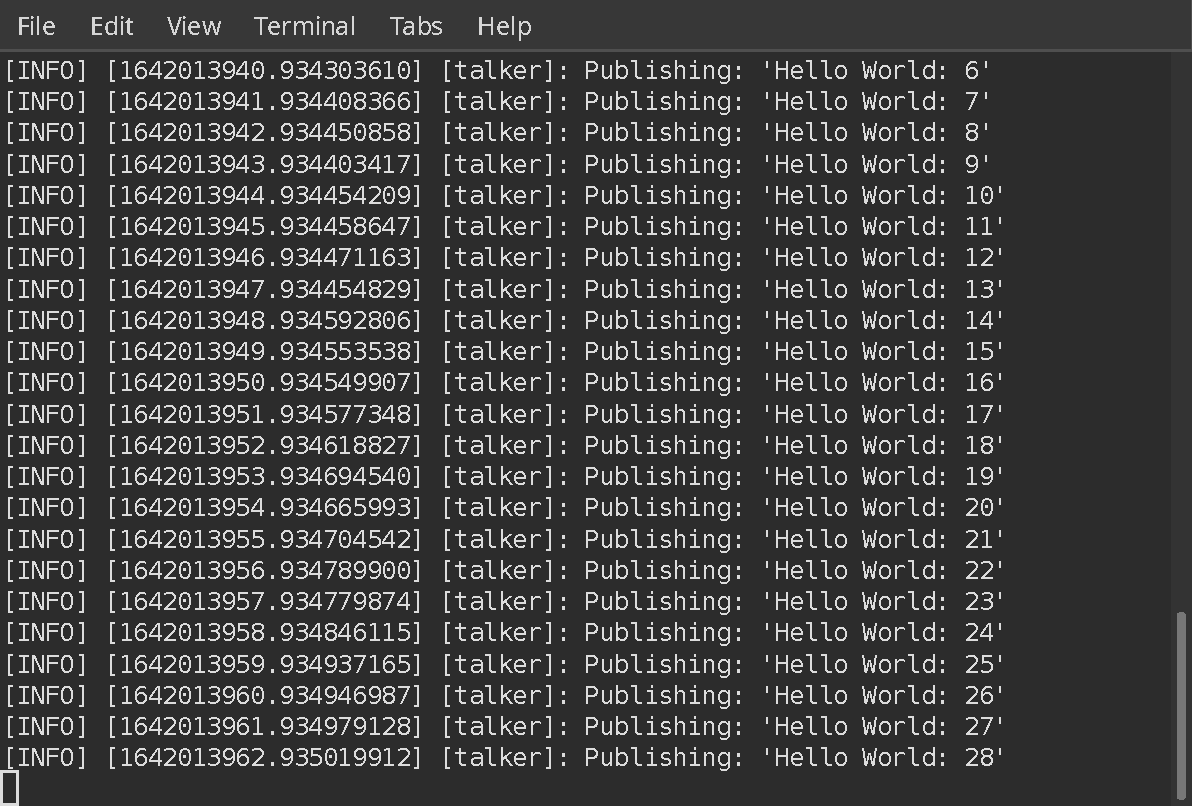
\includegraphics[width=0.48\textwidth]{Talker.pdf}}}\hfill
    \subfloat[Nodos suscriptor]{\label{fig:listener}{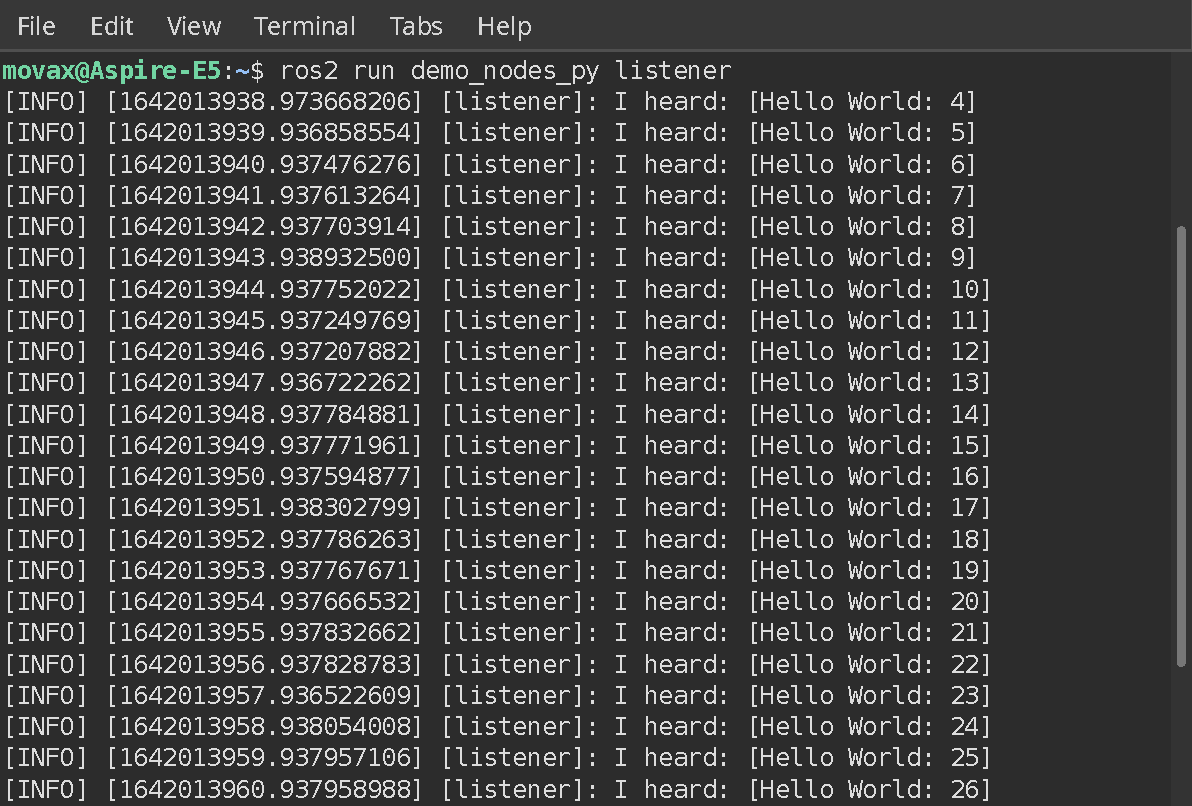
\includegraphics[width=0.48\textwidth]{Listener.pdf}}}
    \caption{Nodos de demostración incluidos en la instalación de ROS 2}
    \label{fig:rosdemo}
\end{figure}

\subsection{Instalación de OpenCV}

Como prerrequisito para instalar la librería de OpenCv es indispensable contar con Python 3 y su gestor de paquetes \textit{pip}. 

La gran mayoría de distribuciones basadas en Ubuntu vienen con Python 3 instalado por defecto. Se puede verificar su instalación con el siguiente comando:

\begin{lstlisting}[language = bash]
    $ python3 --version 
\end{lstlisting}

La expresión anterior debería de imprimir la versión de Python con la que cuenta el sistema, o en su defecto, si Python no se encuentra instalado, se muestra un mensaje que indica que el comando ingresado no existe. Si este último no es el caso, se puede proceder directamente a la instalación de pip.

Instalación de Python 3:
\begin{enumerate}
    \item Actualizar la lista de repositorios del sistema

    \begin{lstlisting}[language = bash]
        $ sudo apt update && sudo apt -y full-upgrade
    \end{lstlisting}
    
    \item Instalar Python 3 desde los repositorios oficiales de Ubuntu

    \begin{lstlisting}[language = bash]
        $ sudo apt install python 3
    \end{lstlisting}

    \item Verificar la instalación de Python

    \begin{lstlisting}[language = bash]
        $ python3 --version 
    \end{lstlisting}

    \item Instalar pip 

    \begin{lstlisting}[language = bash]
        $ sudo apt install python3-pip
    \end{lstlisting}

    \item Verificar instalación de pip

    \begin{lstlisting}[language = bash]
        $ pip3 --version
    \end{lstlisting}
\end{enumerate}

Una vez que se cumplió con el prerrequisito anterior, se puede proceder con la instalación de OpenCV. Cabe mencionar que se aconseja usar ambientes virtuales de Python por cada proyecto, esto con el objetivo de evitar que la instalación de paquetes afecte a otros proyectos desarrollados en el mismo sistema. Sin embargo, debido a que el sistema que utilizado estuvo enfocado exclusivamente a la elaboración de este proyecto, en este trabajo se muestra la instalación global de la librería.

La instalación de la librería es sencilla y se puede realizar con un único comando

\begin{lstlisting}[language = bash]
    $ pip install opencv-contrib-python
\end{lstlisting}

Para verificar la instalación de la librería, se puede ejecutar un pequeño script de Python desde la terminal.

\begin{lstlisting}[language = bash]
    $ python3
    >>> import cv2
    >>> cv2.__version__
\end{lstlisting}

Si la instalación se realizó de forma correcta, se debe de mostrar un mensaje donde se indica la versión de OpenCV que se instaló, como se muestra en la figura \ref{fig:OpenCV_ver}

\begin{figure}[ht]
    \centering
    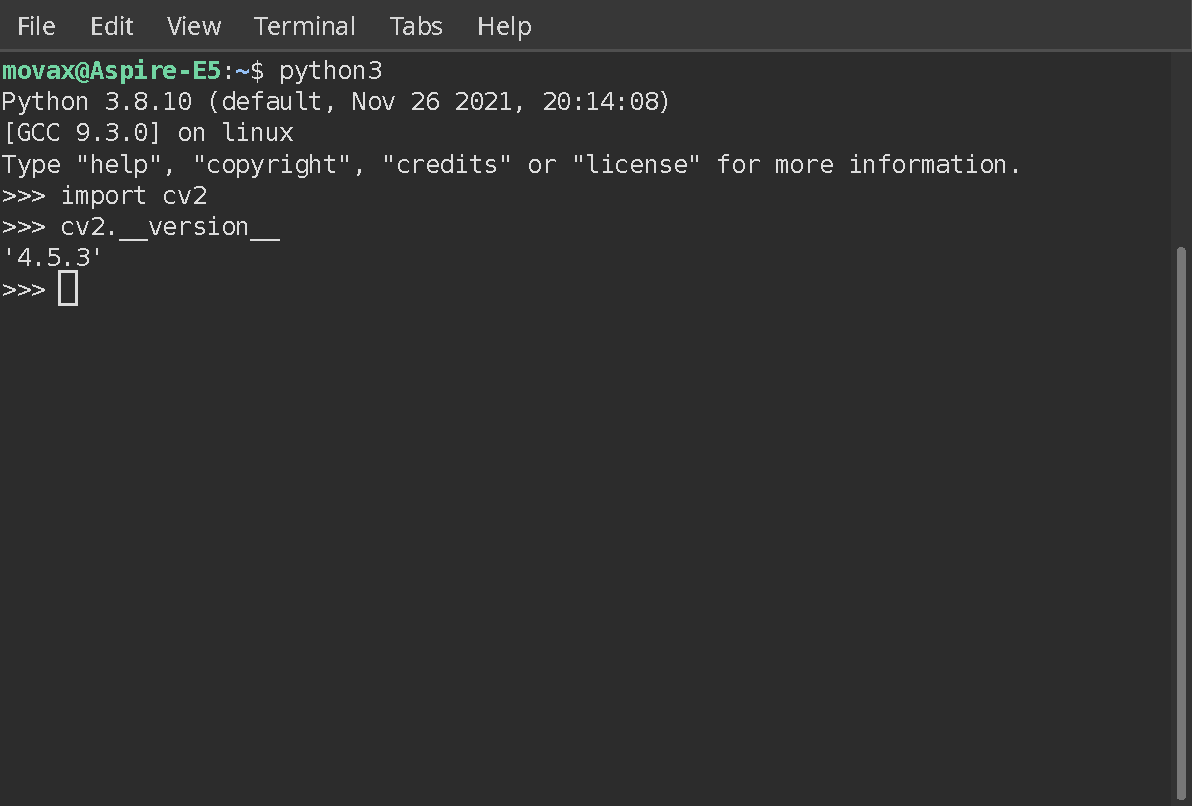
\includegraphics[width=0.6\textwidth]{OpenCV_ver.pdf}
    \caption{Mensaje de validación para la instalación de OpenCV}
    \label{fig:OpenCV_ver}
\end{figure}

\subsection{Instalación de Gazebo}

Como se mencionó en el marco teórico, Gazebo es un ambiente de simulación independiente; es decir, no necesita de ROS o ArduPilot para funcionar. Sin embargo, para habilitar la comunicación entre los nodos de ROS y Gazebo, es recomendable realizar la instalación de Gazebo utilizando los repositorios ofrecidos por ROS 2.

La instalación es sencilla y solo requiere ejecutar el siguiente comando:

\begin{lstlisting}[language = bash]
    $ sudo apt install ros-foxy-gazebo-ros-pkgs
\end{lstlisting}

Al ejecutar la instrucción anterior, se instala en conjunto Gazebo y el plugin para la comunicación entre ROS y Gazebo, \textit{gazebo\_ros\_pkg}. Además, el repositorio también incluye una serie de simulaciones de prueba para demostrar la manera en la que se lleva a cabo la comunicación entre una simulación en Gazebo y un nodo de ROS. 

Por otro lado, cabe destacar que, de la misma forma en la cada versión de ROS es desarrollada para trabajar bajo una versión especifica de Ubuntu, cada versión de ROS también tiene asociada una única versión compatible de Gazebo; para el caso de ROS 2 Foxy, se trabaja con la última versión disponible, Gazebo 11. La figura \ref{fig:Gazebo_ver} muestra los datos técnicos sobre la versión de Gazebo con la que se trabajó.

\begin{figure}[ht]
    \centering
    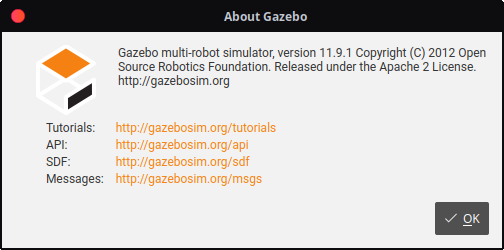
\includegraphics[width=0.5\textwidth]{Gazebo_ver.png}
    \caption{Ficha técnica de la versión de Gazebo}
    \label{fig:Gazebo_ver}
\end{figure}


Una vez que terminó la ejecución del comando anterior, se puede verificar que la instalación se realizó de manera correcta ejecutando Gazebo desde la terminal, tal que

\begin{lstlisting}[language = bash]
    $ gazebo
\end{lstlisting}

La instrucción anterior ejecuta una instancia de Gazebo, en donde al no haber ingresado ningún parámetro para cargar un mundo o ambiente de simulación existente, se abre la pantalla inicial del simulador, con un mundo vacío, tal como se muestra en la figura \ref{fig:Gazebo_world}.

\begin{figure}[ht]
    \centering
    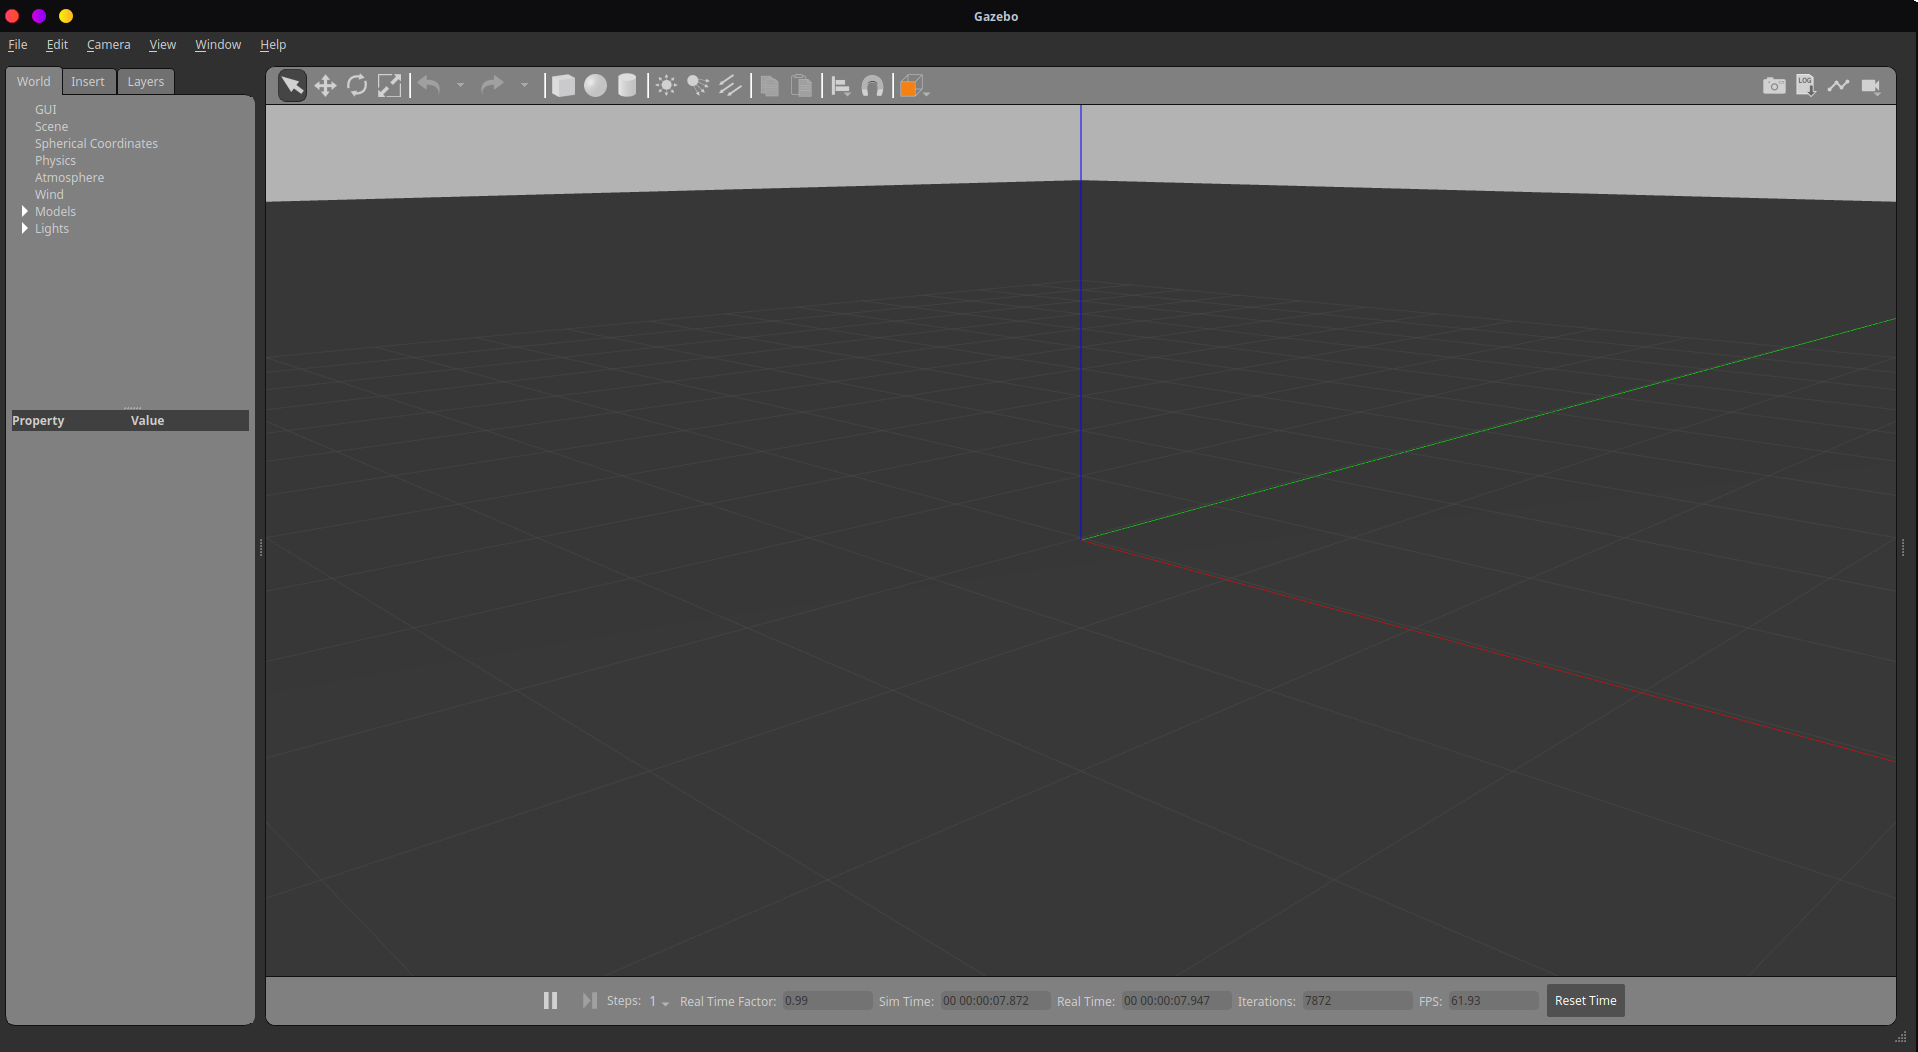
\includegraphics[width=\textwidth]{Gazebo_world.png}
    \caption{Proyecto vacío generado al inicializar Gazebo}
    \label{fig:Gazebo_world}
\end{figure}

Por otro lado, con el fin de comprobar la comunicación entre ROS y Gazebo, se puede ejecutar una de las simulaciones demos incluidas en la instalación. Para ello se selecciona una de las simulaciones más básicas, en donde se tiene un modelo sencillo de un robot y por medio de un topic de ROS se envían instrucciones al robot para su desplazamiento.

Para realizar lo anterior primero se debe de ejecutar una instancia de Gazebo con el mundo que se desea simular.

\begin{lstlisting}[language = bash]
    $ gazebo --verbose /opt/ros/foxy/share/gazebo_plugins/worlds/gazebo_ros_diff_drive_demo.world
\end{lstlisting}

Una vez iniciada la simulación, se pueden enviar instrucciones para el robot por medio de ROS, de la siguiente manera:

\begin{lstlisting}[language = bash]
    $ ros2 topic pub /demo/cmd_demo geometry_msgs/Twist '{linear: {x: 1.0}}' -1
\end{lstlisting}

\begin{figure}[ht]
    \centering
    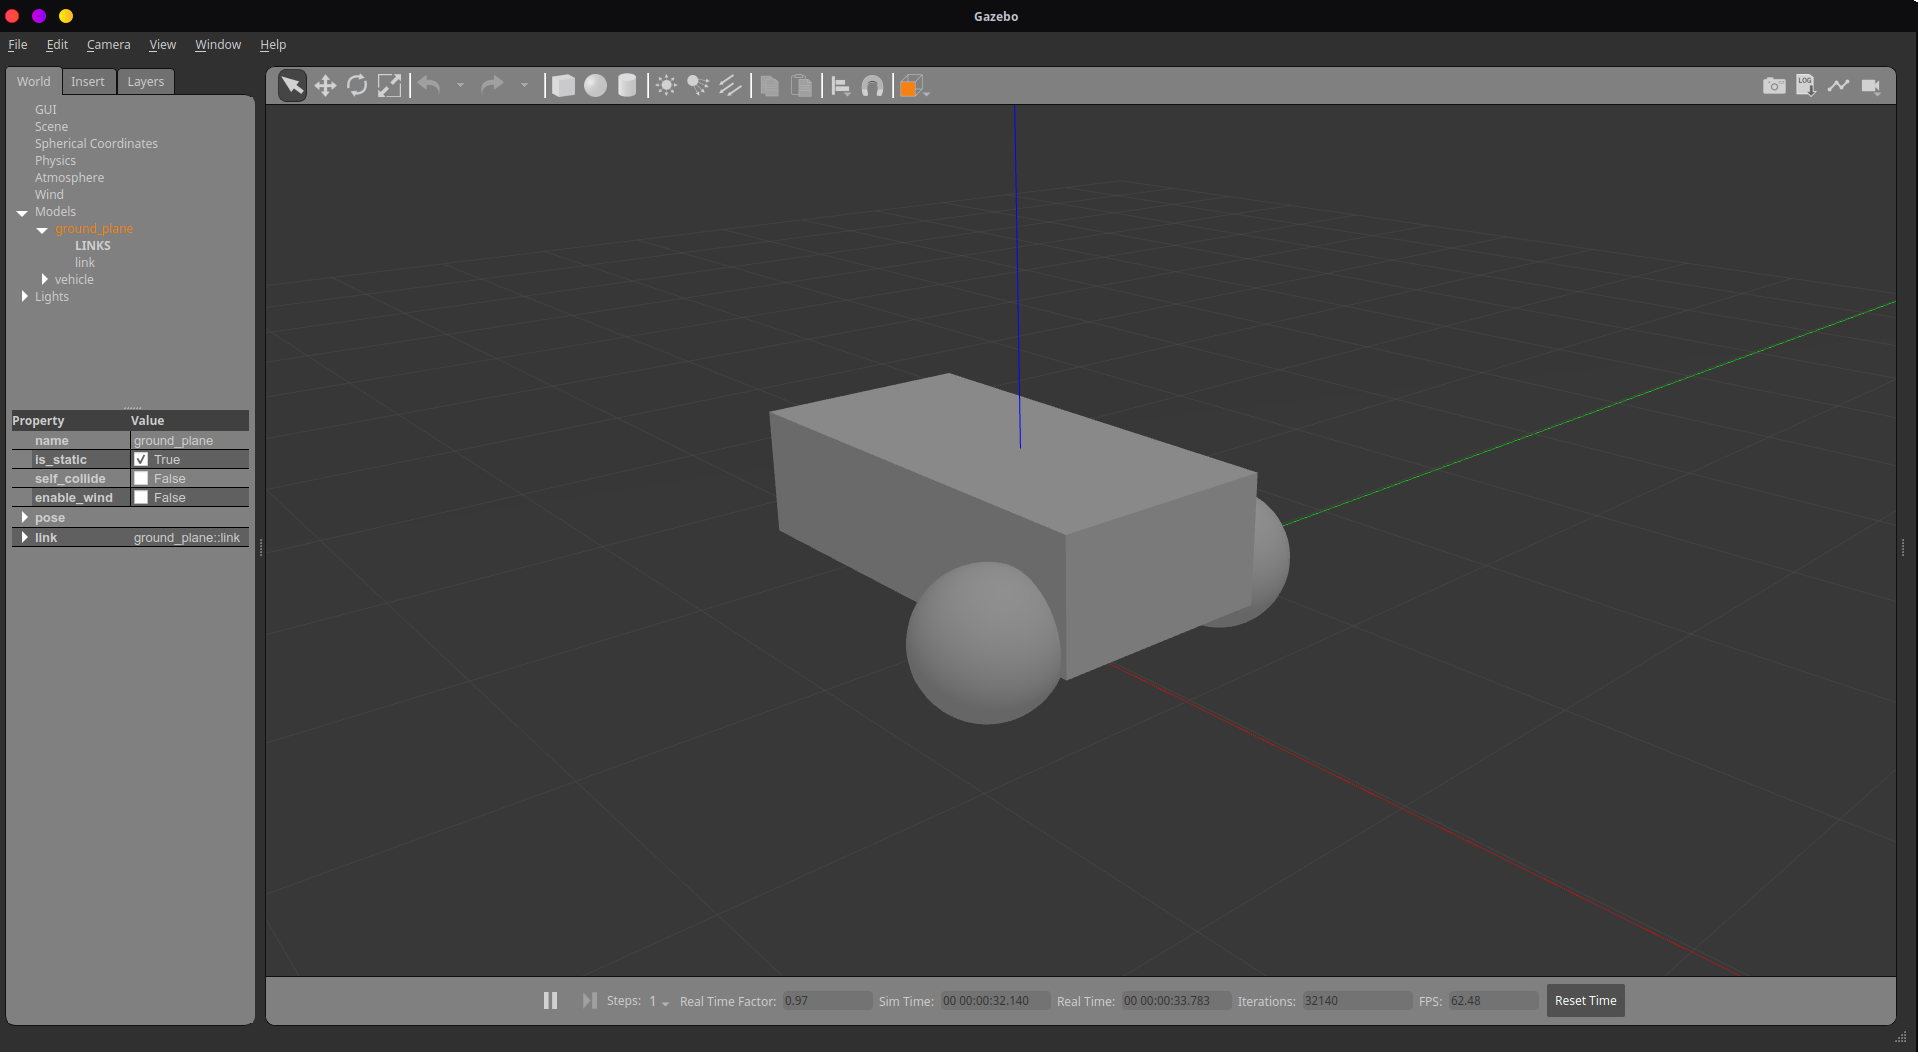
\includegraphics[width=\textwidth]{Gazebo_ros.png}
    \caption{Proyecto de demostración en Gazebo que incluye el plug-in para comunicarse con ROS}
    \label{fig:Gazebo_ros}
\end{figure}

La figura \ref{fig:rossims} muestra el movimiento observado en la simulación  a partir de haber ingresado un comando por medio de la API de ROS.

\begin{figure}[ht]
    \centering
    \subfloat[Primera posición]{\label{fig:rossim1}{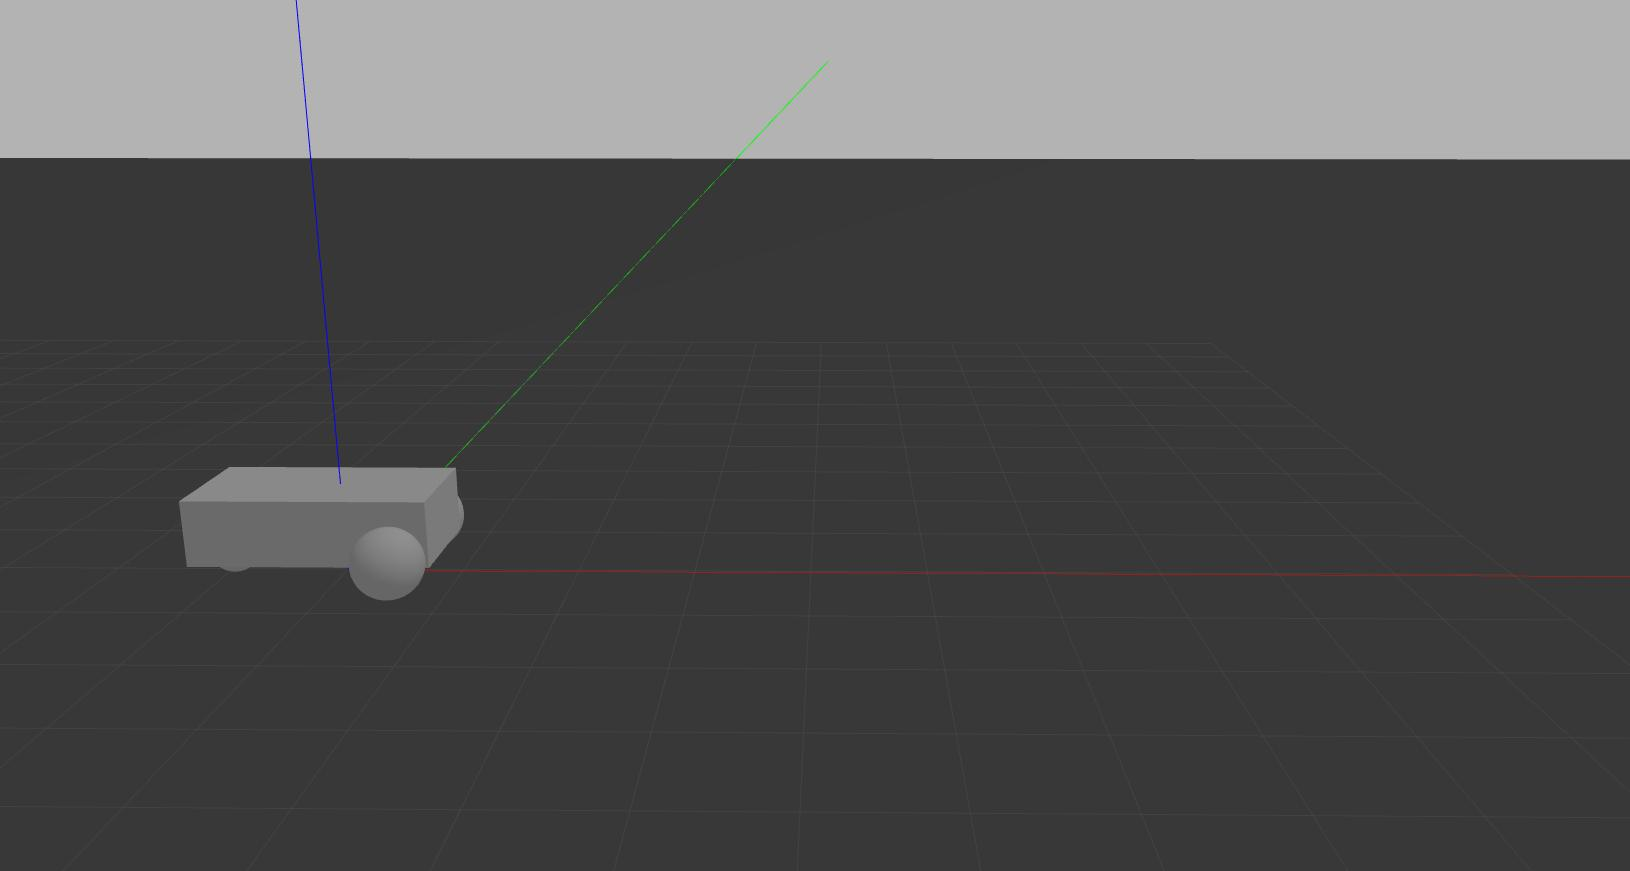
\includegraphics[width=0.48\textwidth]{ROS_sim1.jpg}}}\hfill
    \subfloat[Segunda posición]{\label{fig:rossim2}{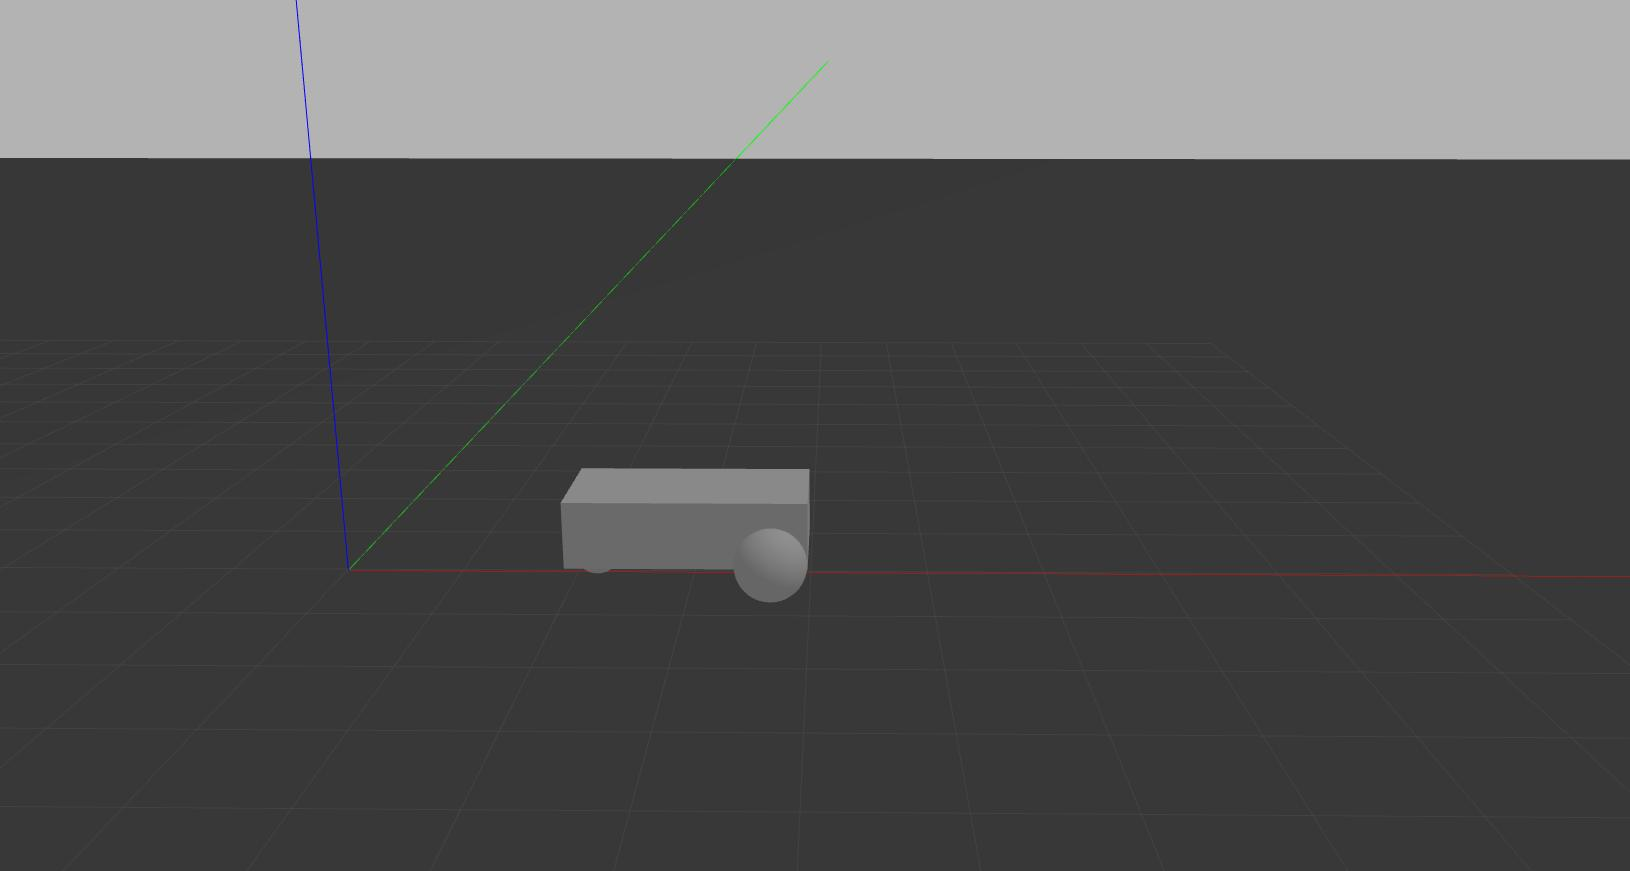
\includegraphics[width=0.48\textwidth]{ROS_sim2.jpg}}}\\
    \subfloat[Tercera posición]{\label{fig:rossim3}{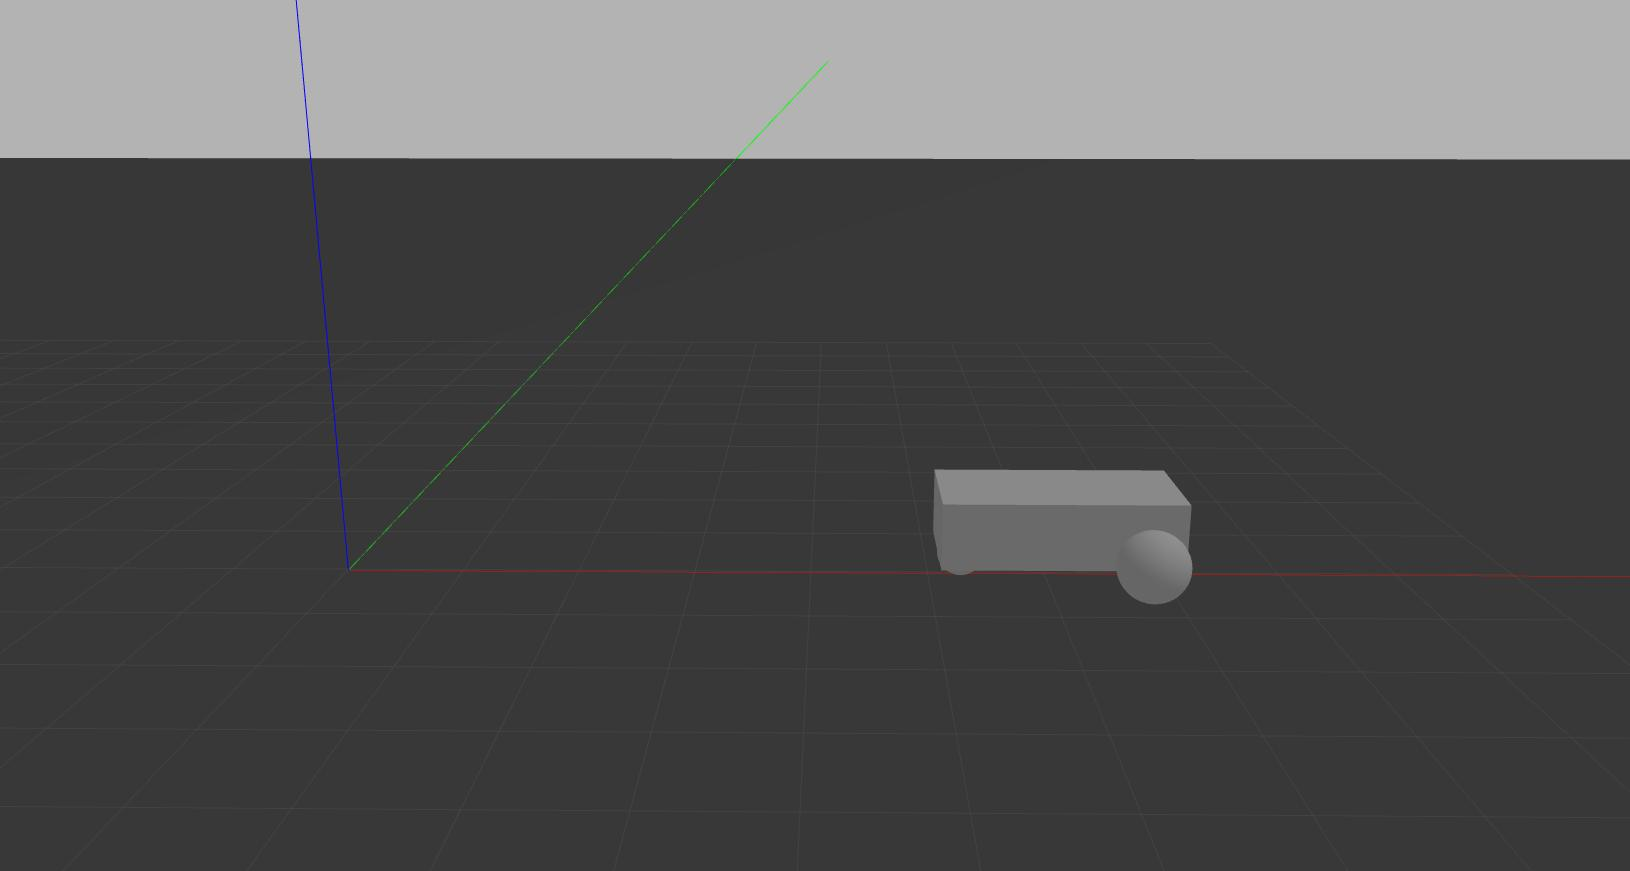
\includegraphics[width=0.48\textwidth]{ROS_sim3.jpg}}}\hfill
    \subfloat[Cuarta posición]{\label{fig:rossim4}{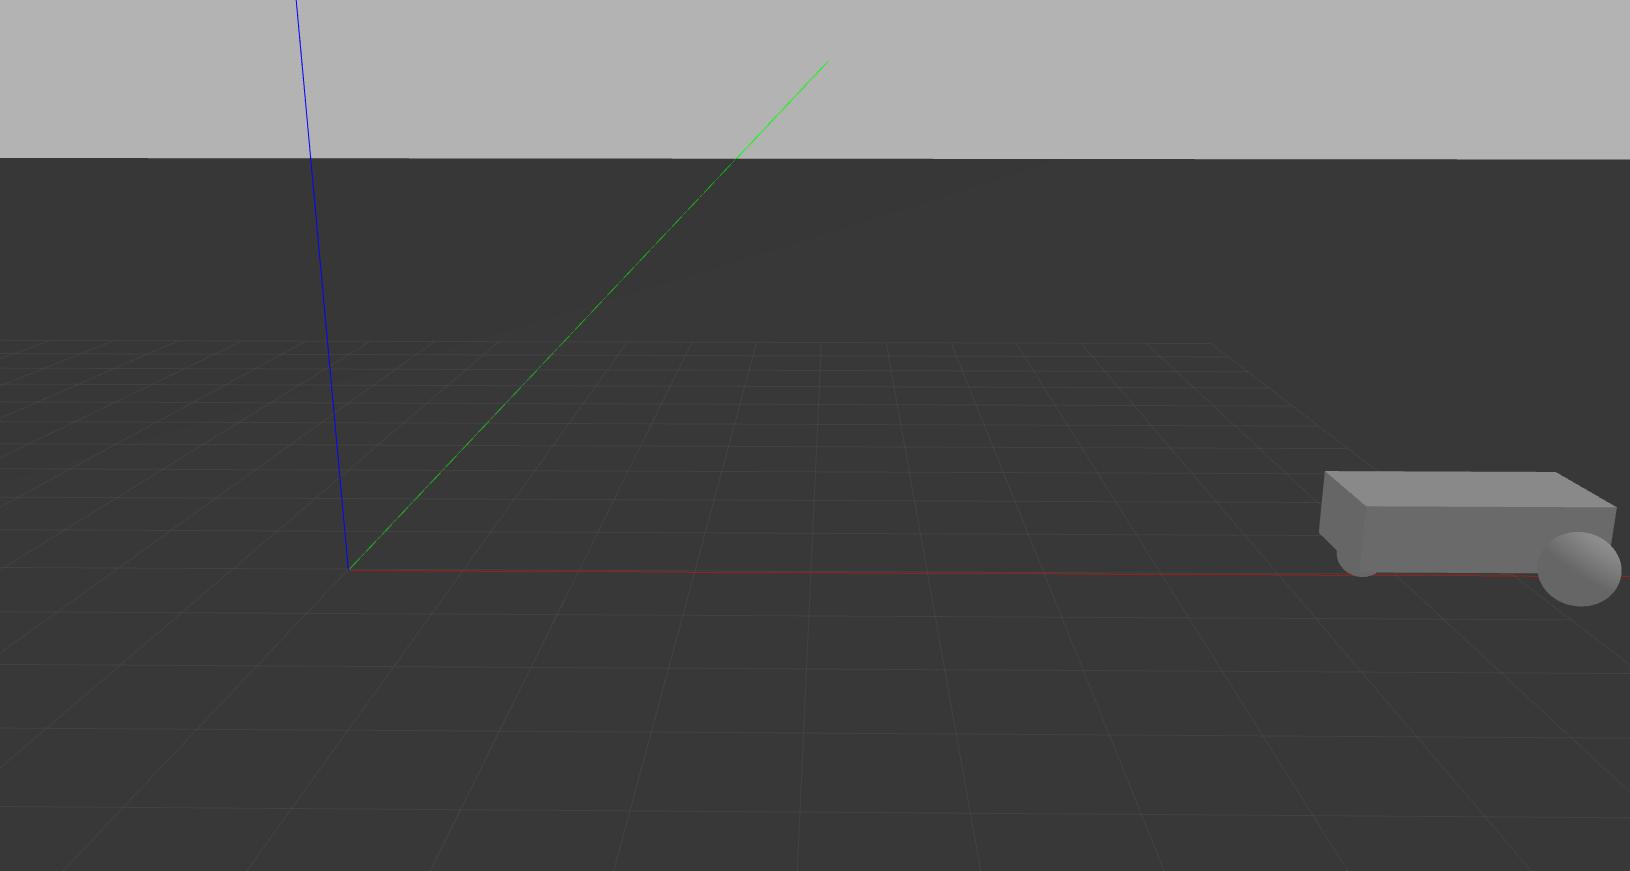
\includegraphics[width=0.48\textwidth]{ROS_sim4.jpg}}}
    \caption{Movimiento de la simulación en Gazebo con plugin de comunicación de ROS}
    \label{fig:rossims}
\end{figure}


Para consultar el resto de simulaciones de demostración incluida, se puede acceder al directorio donde se encuentra instalado ROS y listar los nombre de las simulaciones instaladas. Es posible abrir los archivos de simulación con un editor de texto y observar la documentación incluida en cada una, en donde se especifica el modo de uso de esta, la interfaz de mensajes que utilizar para la comunicación y la sintaxis necesaria para enviar mensajes utilizando ROS.

\begin{lstlisting}[language = bash]
    $ cd  /opt/ros/foxy/share/gazebo_plugins/worlds
    $ ls 
\end{lstlisting}

\begin{figure}[ht]
    \centering
    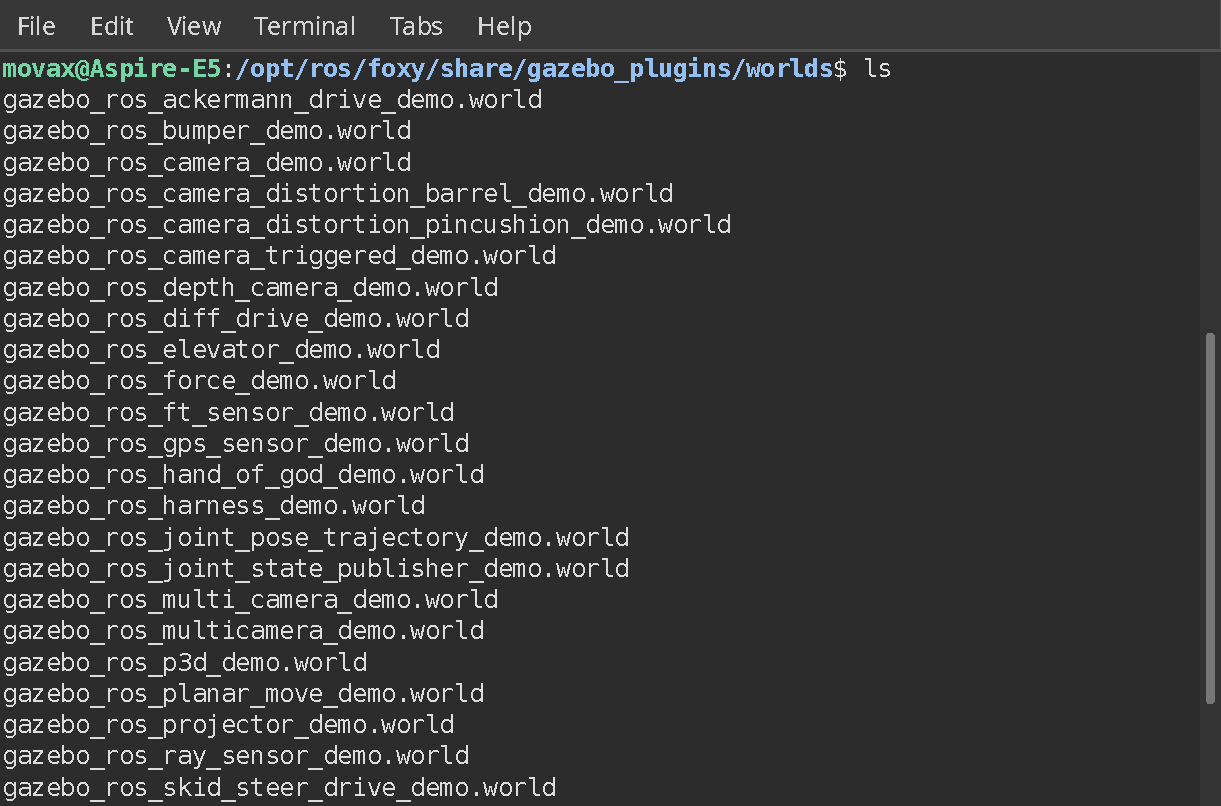
\includegraphics[width=0.6\textwidth]{ROS_demos.pdf}
    \caption{Lista de simulaciones de demostración para el uso de Gazebo con ROS 2}
    \label{fig:ROS_demos}
\end{figure}

\subsection{Instalación de ArduPilot SIL Simulator}
Configurar y trabajar con el framework de simulación de ArduPilot es quizás la parte más compleja en cuanto al software utilizado para el sistema propuesto. Esto es debido a que la gran parte de la documentación oficial se encuentra desactualizada y los recursos que proveen información al respecto se encuentran dispersos por foros y otros tipos de documentación no oficial. 

A continuación se muestra una síntesis del proceso de instalación y Configuración para ArduPilot SIL Simulator.

\begin{enumerate}

    \item Ubicarse en el directorio donde se desean almacenar los archivos del repositorio de ArduPilot y clonar el proyecto.

    \begin{lstlisting}[language = bash]
        $ git clone --recursive https://github.com/ArduPilot/arduPilot.git
        $ cd arduPilot
    \end{lstlisting}    

    \item Instalar las herramientas necesarias para la compilación de ArduPilot
    
    \begin{lstlisting}[language = bash]
        $ Tools/environment_install/install-prereqs-ubuntu.sh -y
    \end{lstlisting}   

    \item Recargar la ruta de trabajo para hacer uso de las herramientas
    
    \begin{lstlisting}[language = bash]
        $ . ~/.profile
    \end{lstlisting}   

    \item Compilar el paquete seleccionando el modelo de computadora de vuelo y el vehículo deseado.

    \begin{lstlisting}[language = bash]
        $ ./waf configure --board CubeBlack
        $ ./waf copter
    \end{lstlisting}

    Como comentario complementario, ArduPilot es compatible con varios modelos de computadoras de vuelo, en este caso se seleccionó una \textit{Pixhawk2 Cube}. Para obtener el listado de todas las computadoras de vuelo compatibles, se puede ejecutar la siguiente instrucción; de tal forma que es posible seleccionar cualquier otro modelo cambiando el nombre del parámetro por cualquier de la lista. 

    \begin{lstlisting}[language = bash]
        $ ./waf list_boards
    \end{lstlisting}

    De igual manera, el parámetro de vehículo puede ser modificado por el nombre de otro de los vehículos con los que trabaja ArduPilot, acorde a las necesidades del usuario. Para enlistar los vehículos disponibles se puede utilizar el comando \textit{"list"}.
    
    \begin{lstlisting}[language = bash]
        $ ./waf list
    \end{lstlisting}

    \item Limpiar los archivos temporales generados tras la compilación.
    
    \begin{lstlisting}[language = bash]
        $ ./waf clean
    \end{lstlisting}

    \item Añadir el API de ArduPilot al perfil de bash
    
    \begin{lstlisting}[language = bash]
        $ echo "export PATH=$PATH:$HOME/ardupilot/Tools/autotest" >> ~/.bashrc
        $ echo "export PATH=/usr/lib/ccache:$PATH" >> ~/.bashrc 
    \end{lstlisting}  

    \item Recargar el directorio de trabajo con el nuevo perfil de bash
    
    \begin{lstlisting}[language = bash]
        $ . ~/.bashrc
    \end{lstlisting}  

\end{enumerate}

Hecho lo anterior, se puede realizar la prueba del  framework de SIL, para ello es necesario dirigirse al directorio del vehículo instalado, dentro del directorio donde se descargó ArduPilot. 

\begin{lstlisting}[language = bash]
    $ cd ~/ardupilot/ArduCopter
\end{lstlisting}  

Una vez dentro del directorio, se puede ejecutar la simulación del vehículo con el siguiente comando:

\begin{lstlisting}[language = bash]
    $ sim_vehicle.py --map --console
\end{lstlisting}  


El comando anterior ejecuta una instancia del SIL de ArduPilot, de tal forma que se abren dos ventanas; un mapa una terminal.

La terminal que se abre al momento de ejecutar la simulación corresponde a la consola de vuelo, en esta se indican algunos parámetros de interés del dron, tal como el nivel de la batería, el modo de vuelo, la altura a la que se encuentra, un historial de eventos, entre otras cosas.

El mapa contiene un pequeño esquema de un cuadricóptero (vehículo compilado para este trabajo) y es donde se puede observar su desplazamiento con base en los comandos ingresados a partir de la terminal de ArduPilot.

Es posible controlar el dron utilizando comandos ingresados desde la terminal o directamente utilizando el mapa. Es posible asignar waypoints y rutas de vuelo de forma gráfica dando clic derecho sobre el mapa.

A continuación se adjuntan una serie de comandos ejemplo para realizar un desplazamiento básico, en donde el dron despega 10 m sobre el suelo y luego se mueve otros 20 m en el eje x.

Se debe de ingresar lo siguiente en la terminal desde donde se inició la sesión de ArduPilot:

\begin{lstlisting}[language = bash]
    > mode guided     #cambia el modo de vuelo
    > arm throttle    #arma los motores del dron
    > takeoff 10      #despegue
    > position 50 0 0 #desplazamiento en x,y,z
\end{lstlisting}  

Lo anterior corresponde a una demostración del uso básico del simulador standalone de ArduPilot; sin embargo, en este trabajo se propone Gazebo como ambiente de simulación, por lo que es necesario conectar el SIL de Ardupilot con este simulador. Lo anterior es posible realizando la instalación de un plugin específicamente diseñado con este propósito.


\begin{figure}[ht]
    \centering
    \subfloat[Posición inicial]{\label{fig:Ardupilot_gc}{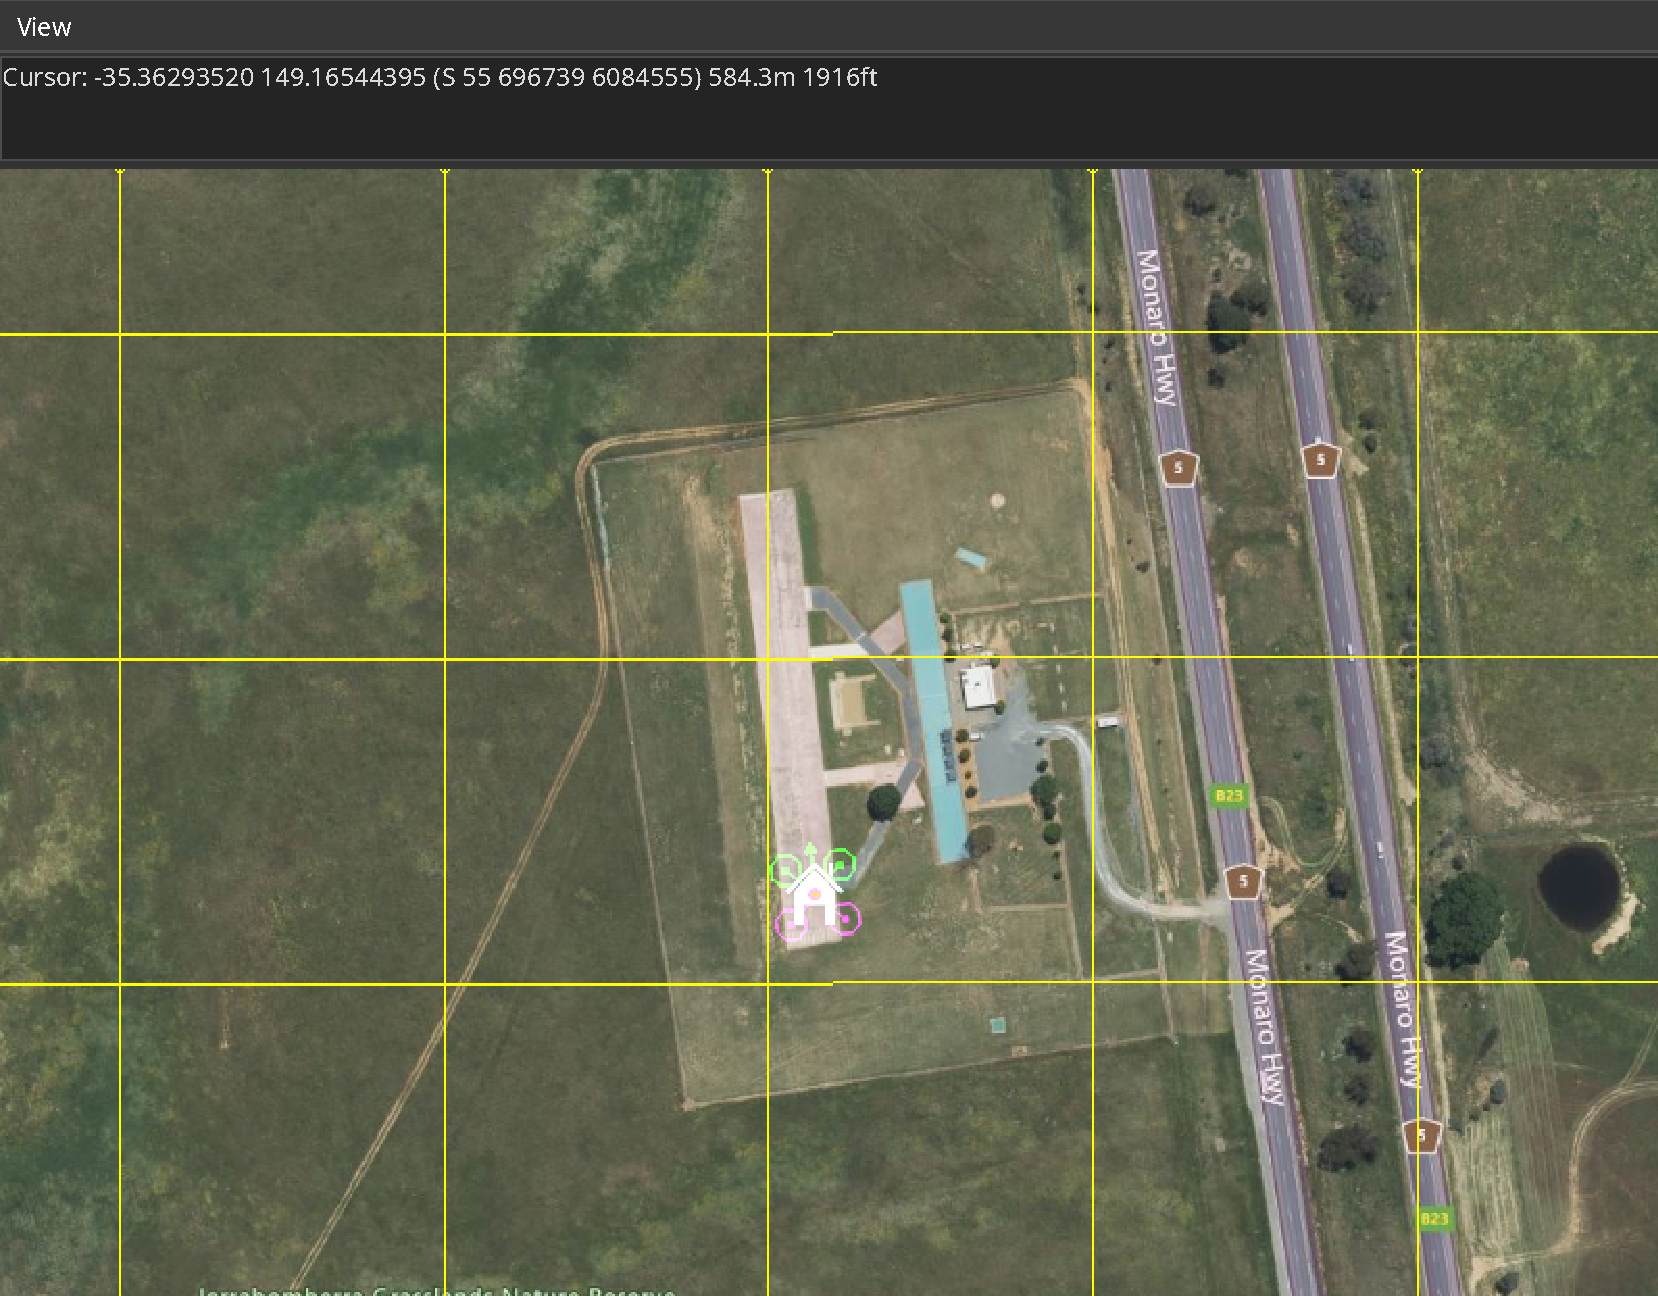
\includegraphics[width=0.48\textwidth]{Ardupilot_gc.pdf}}}\hfill
    \subfloat[Posición final]{\label{fig:Ardupilot_gc1}{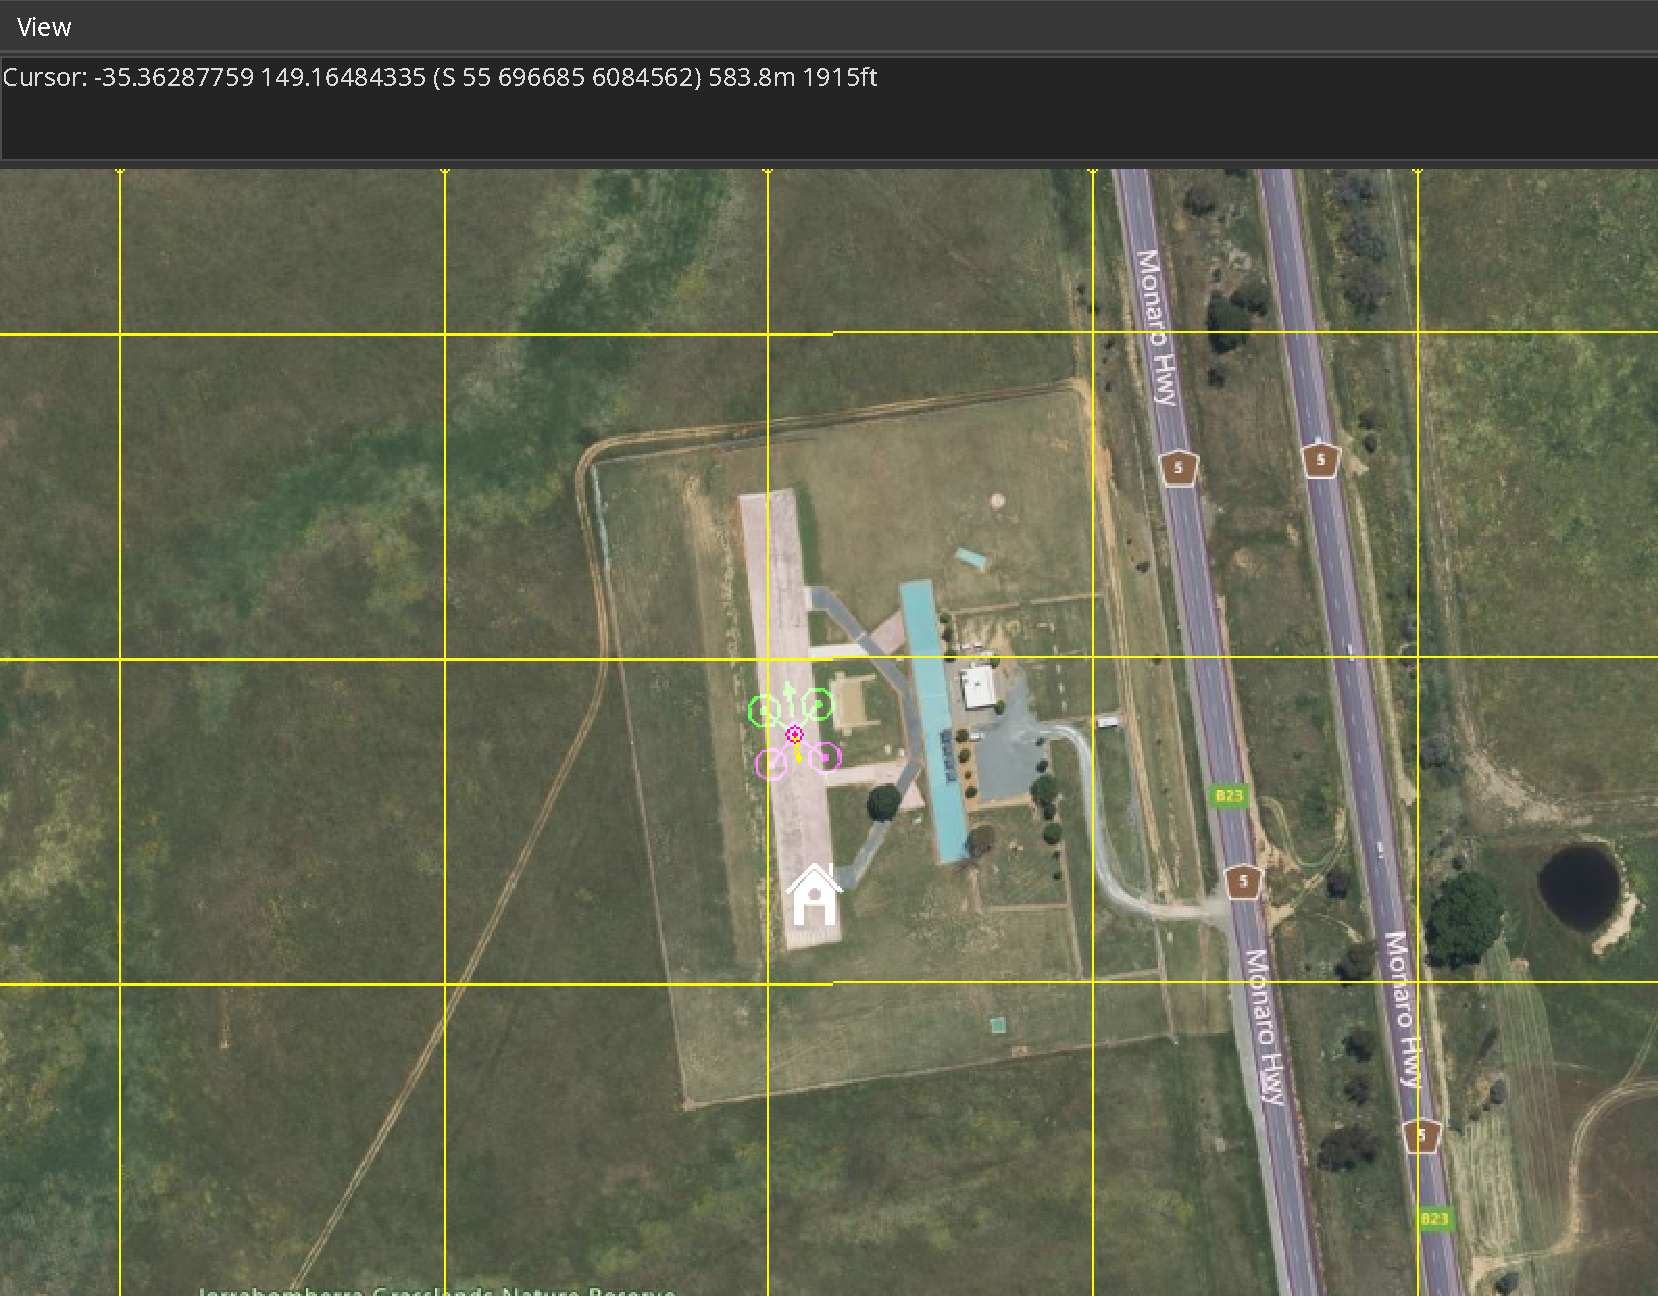
\includegraphics[width=0.48\textwidth]{Ardupilot_gc1.pdf}}}\\
    \subfloat[Terminal con comando de vuelo]{\label{fig:Ardupilot_gcterminal}{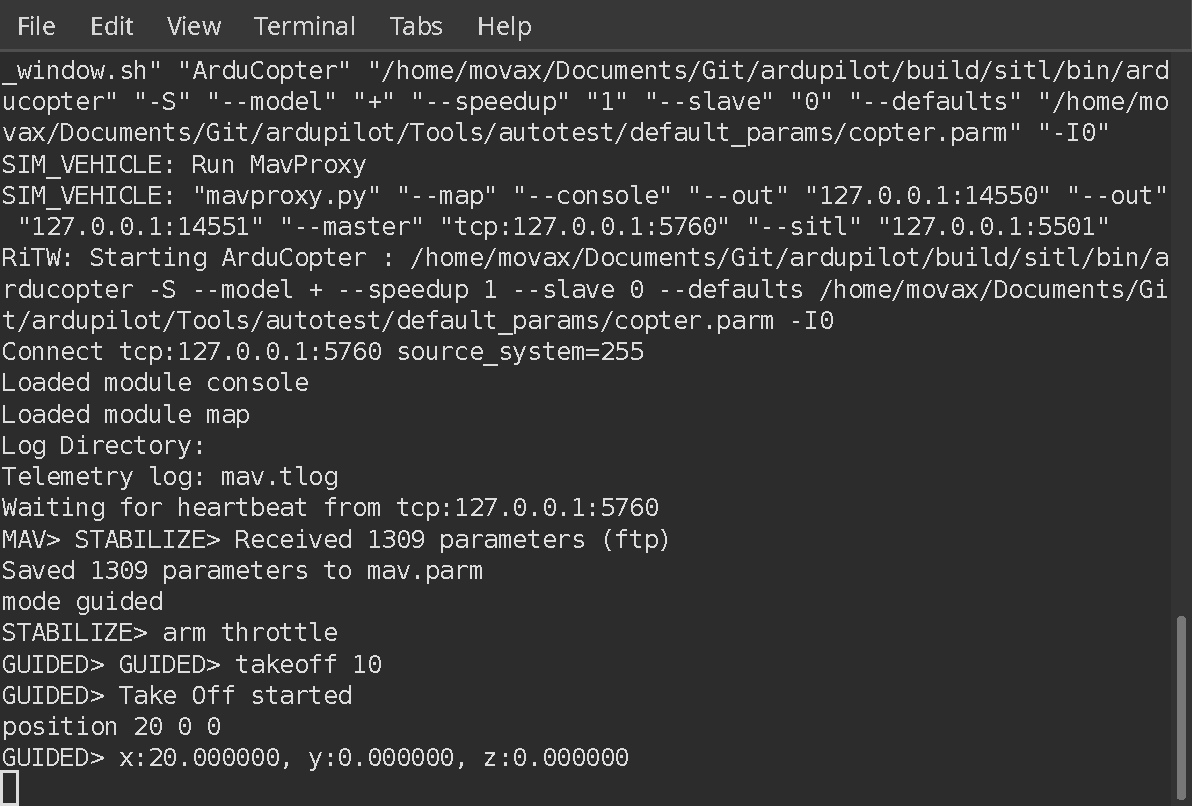
\includegraphics[width=0.5\textwidth]{Ardupilot_gcterminal.pdf}}}\hfill
    \caption{Prueba de ejecución del framework de SIL de ArduPilot}
    \label{fig:Ardupilot}
\end{figure}

\begin{figure}[ht]
    \centering
    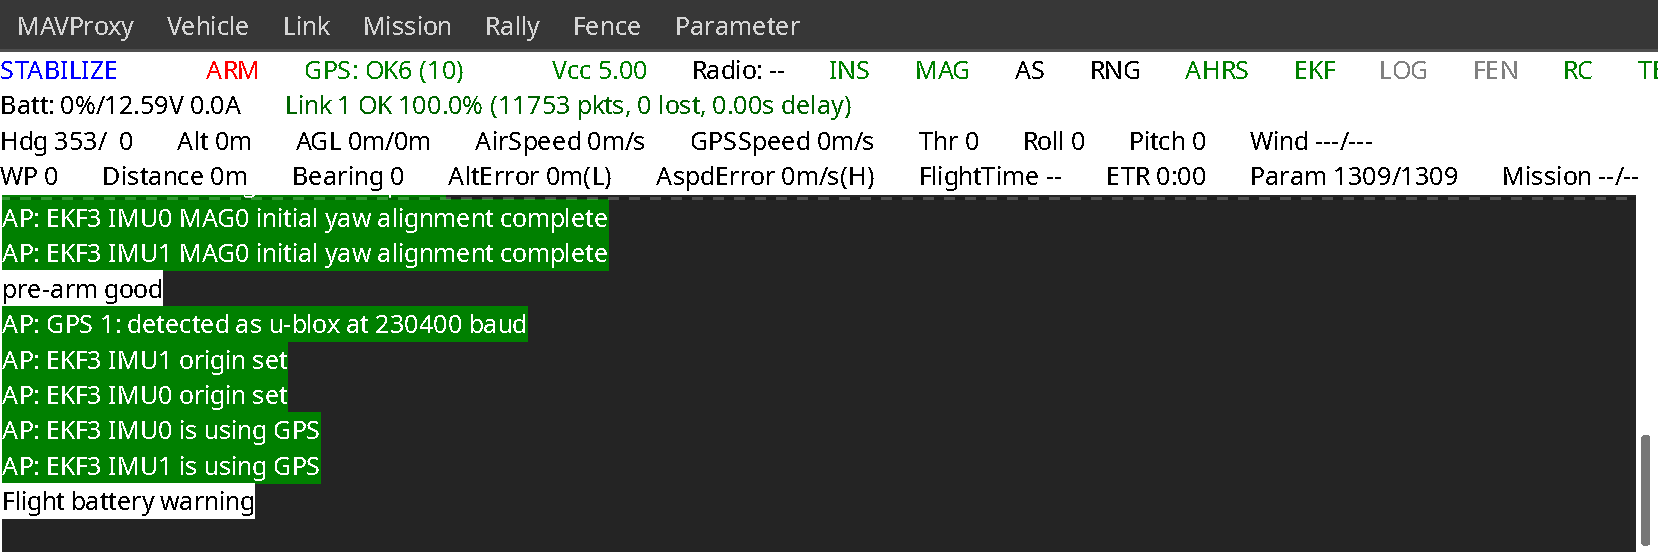
\includegraphics[width=0.8\textwidth]{Ardupilot_mavproxy.pdf}
    \caption{Terminal de información del sistema de ArduPilot}
    \label{fig:Ardupilot_mavproxy}
\end{figure}

\begin{figure}[ht]
    \centering
    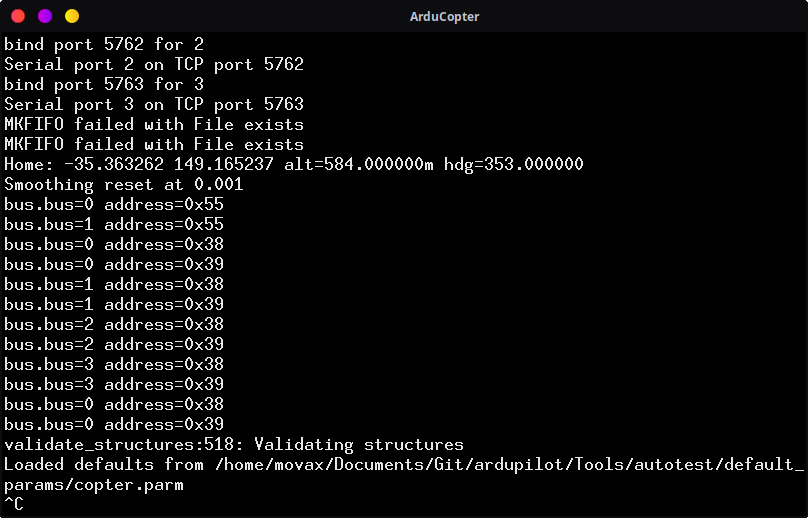
\includegraphics[width=0.8\textwidth]{Ardupilot_console.png}
    \caption{Consola de comunicación de ArduPilot}
    \label{fig:Ardupilot_console}
\end{figure}


Instalación de ArduPilot Gazebo plugin:

\begin{enumerate}
    \item Dirigirse al directorio deseado para descargar al proyecto y clonar el repositorio de Github

    \begin{lstlisting}[language = bash]
        $ git clone https://github.com/khancyr/ardupilot_gazebo
        $ cd ardupilot_gazebo
    \end{lstlisting}  

    \item Compilar el proyecto

    \begin{lstlisting}[language = bash]
        $ mkdir build
        $ cd build
        $ cmake ..
        $ make -j4
        $ sudo make install
    \end{lstlisting} 

    \item Añadir la configuración de Gazebo al perfil de bash

    \begin{lstlisting}[language = bash]
        $ echo 'source /usr/share/gazebo/setup.sh' >> ~/.bashrc
        $ echo 'export GAZEBO_MODEL_PATH=~/ardupilot_gazebo/models' >> ~/.bashrc
        $ echo 'export GAZEBO_RESOURCE_PATH=~/ardupilot_gazebo/worlds:${GAZEBO_RESOURCE_PATH}' >> ~/.bashrc
    \end{lstlisting} 

    \item Recargar la ruta de trabajo con el nuevo perfil de bash
    
    \begin{lstlisting}[language = bash]
        $ source ~/.bashrc
    \end{lstlisting} 

\end{enumerate}

Con la configuración realizada hasta este punto, el sistema del usuario debe de ser capaz de iniciar una instancia de ArduPilot y conectarla con una simulación en Gazebo, de tal forma que los comando ingresados por medio de la terminal de ArduPilot tengan efecto dentro de la simulación de Gazebo. 

La instalación del plugin incluye una simulación de demostración para verificar la comunicación entre ambos programas; sin embargo, al momento de la escritura de este trabajo existe un bug al trabajar la simulación de prueba con Gazebo 11. 
La simulación de demostración integra un modelo 3D de un dron \text{Iris}, el cual viene configurado de tal manera que incluye la dinámica del dron y una serie de sensores simulados, entre ellos una cámara monocular; dicho lo anterior, el bug consiste en no permitir que se cargue el modelo del dron dentro de la simulación, por lo que la comunicación entre los programas no se puede llevar a cabo.

Para corregir lo anterior, es necesario realizar una pequeña modificación dentro del archivo del modelo del dron:

\begin{enumerate}
    \item Ir al directorio donde se encuentra el modelo del dron con el plugin de Ardupilot para Gazebo
    \begin{lstlisting}[language = bash]
        $ cd /usr/share/gazebo-11/models/iris_with_ardupilot
    \end{lstlisting} 
    \item Abrir el archivo \textit{model.sdf} con nano con permisos de superusuario
    \begin{lstlisting}[language = bash]
        $ sudo nano model.sdf
    \end{lstlisting} 
    \item La segunda línea del archivo debe de contener lo siguiente:
    \begin{lstlisting}[language = bash]
        <sdf version="1.7" xmlns:xacro='http://ros.org/wiki/xacro'>
    \end{lstlisting} 
    \item Modificar la línea de código anterior de la siguiente manera
    \begin{lstlisting}[language = bash]
        <sdf version="1.7">
    \end{lstlisting}  
    \item Guardar los cambios y cerrar el archivo
\end{enumerate}

Con la corrección anterior, el usuario debe de ser capaz de ejecutar la simulación de demostración en Gazebo que incluye el plugin de SIL de ArduPilot, de la siguiente manera:

\begin{enumerate}
    \item Abrir 2 terminales
    \item Ejecutar el SIL de ArduPilot en una de las terminales
    \begin{lstlisting}[language = bash]
        cd ~/ardupilot/ArduCopter
    \end{lstlisting}  
    \begin{lstlisting}[language = bash]
        sim_vehicle.py -f gazebo-iris --console
    \end{lstlisting} 
    \item Ejecutar la simulación de Gazebo en la segunda terminal
    \begin{lstlisting}[language = bash]
        gazebo --verbose worlds/iris_arducopter_runway.world
    \end{lstlisting} 
    \item Esperar a que esté listo para recibir comandos de vuelo
    \item Ejecutar los comandos de vuelo utilizados para validar la instalación del SIL de ArduPilot
\end{enumerate}

\begin{figure}[ht]
    \centering
    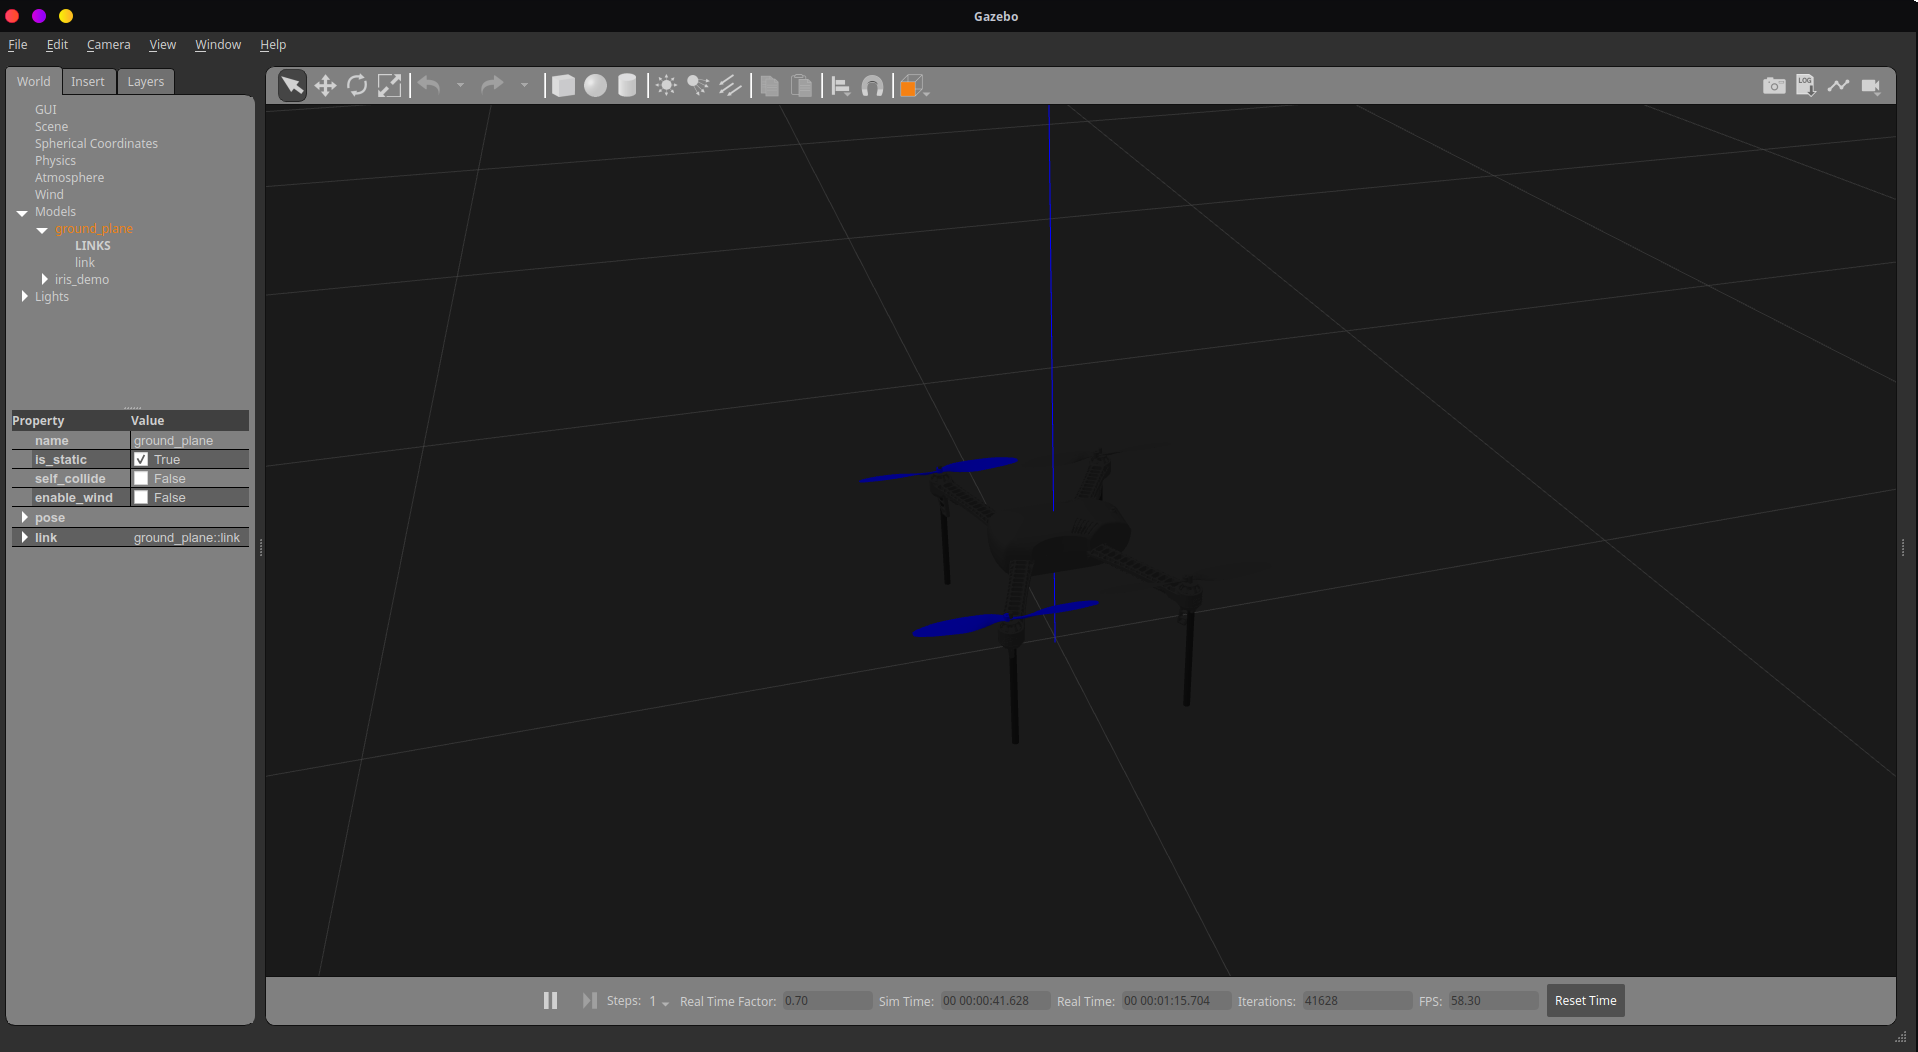
\includegraphics[width=\textwidth]{Gazebo_SITL.png}
    \caption{Modelo en Gazebo del dron Iris}
    \label{fig:Gazebo_SIL}
\end{figure}

\begin{figure}[ht]
    \centering
    \subfloat[Posición inicial]{\label{fig:Ardupilot_sim1}{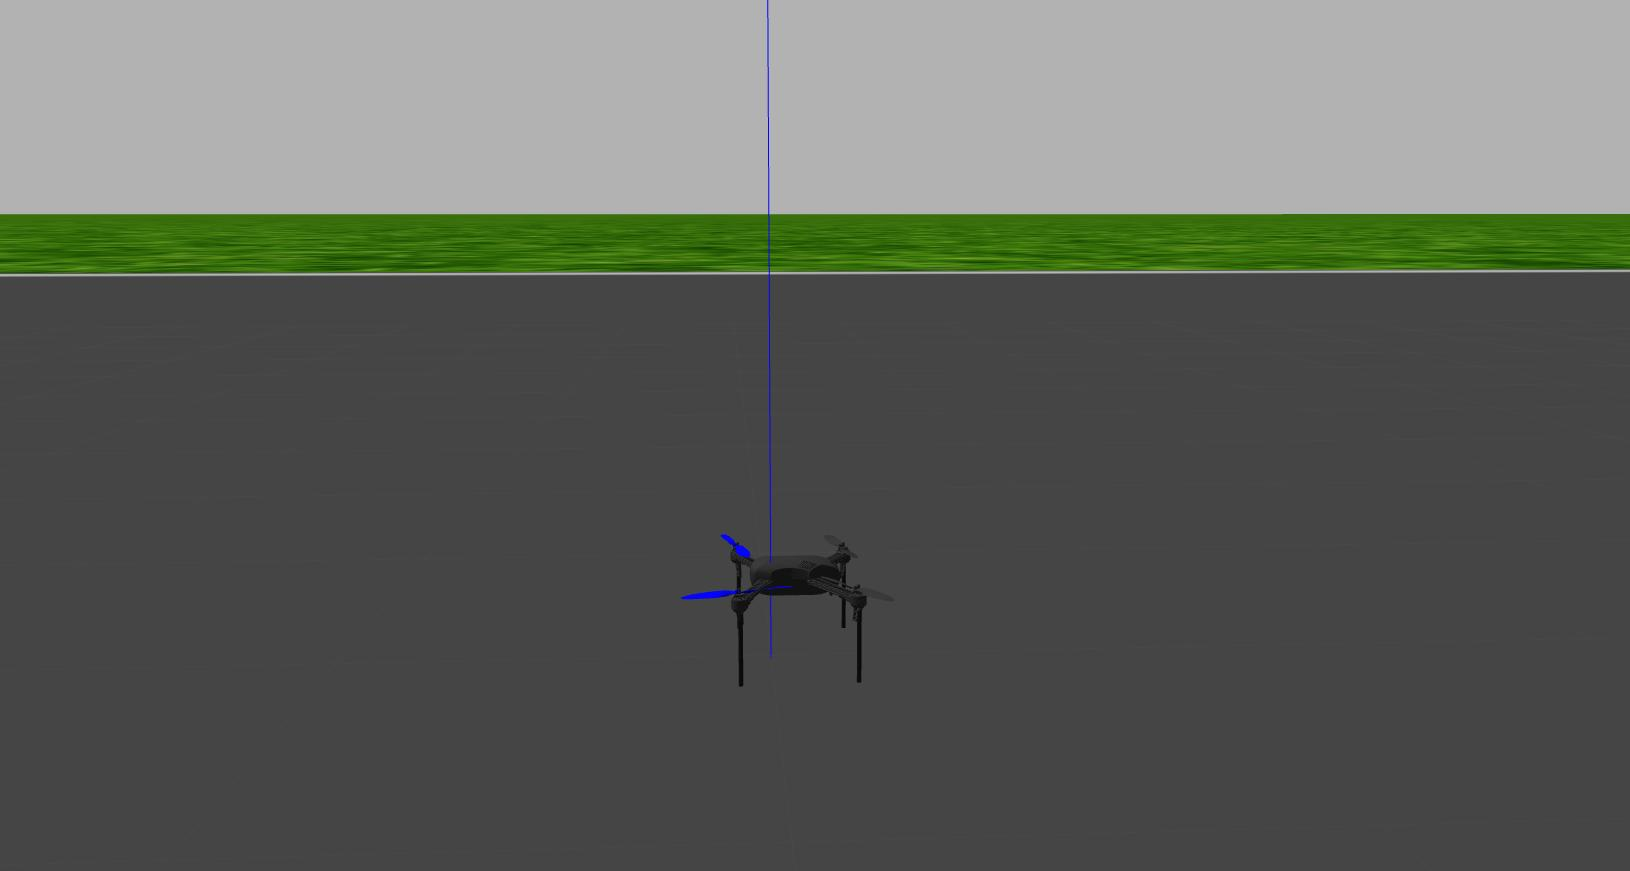
\includegraphics[width=0.48\textwidth]{Ardupilot_sim1.jpg}}}\hfill
    \subfloat[Despegue]{\label{fig:Ardupilot_sim2}{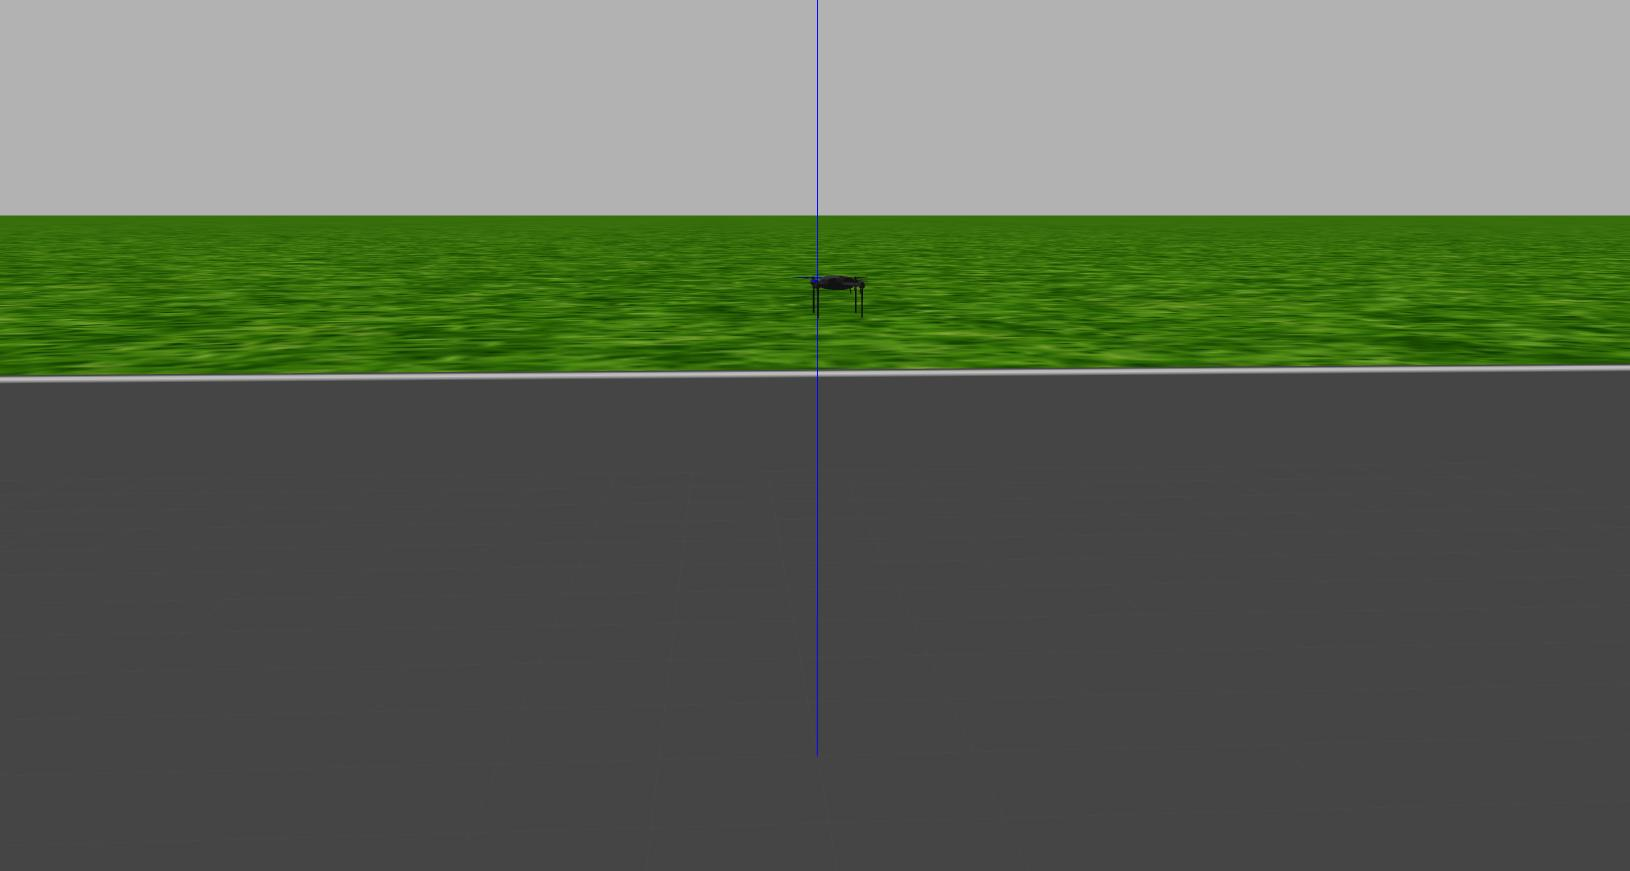
\includegraphics[width=0.48\textwidth]{Ardupilot_sim2.jpg}}}\\
    \subfloat[Movimiento de 20 m en x]{\label{fig:Ardupilot_sim3}{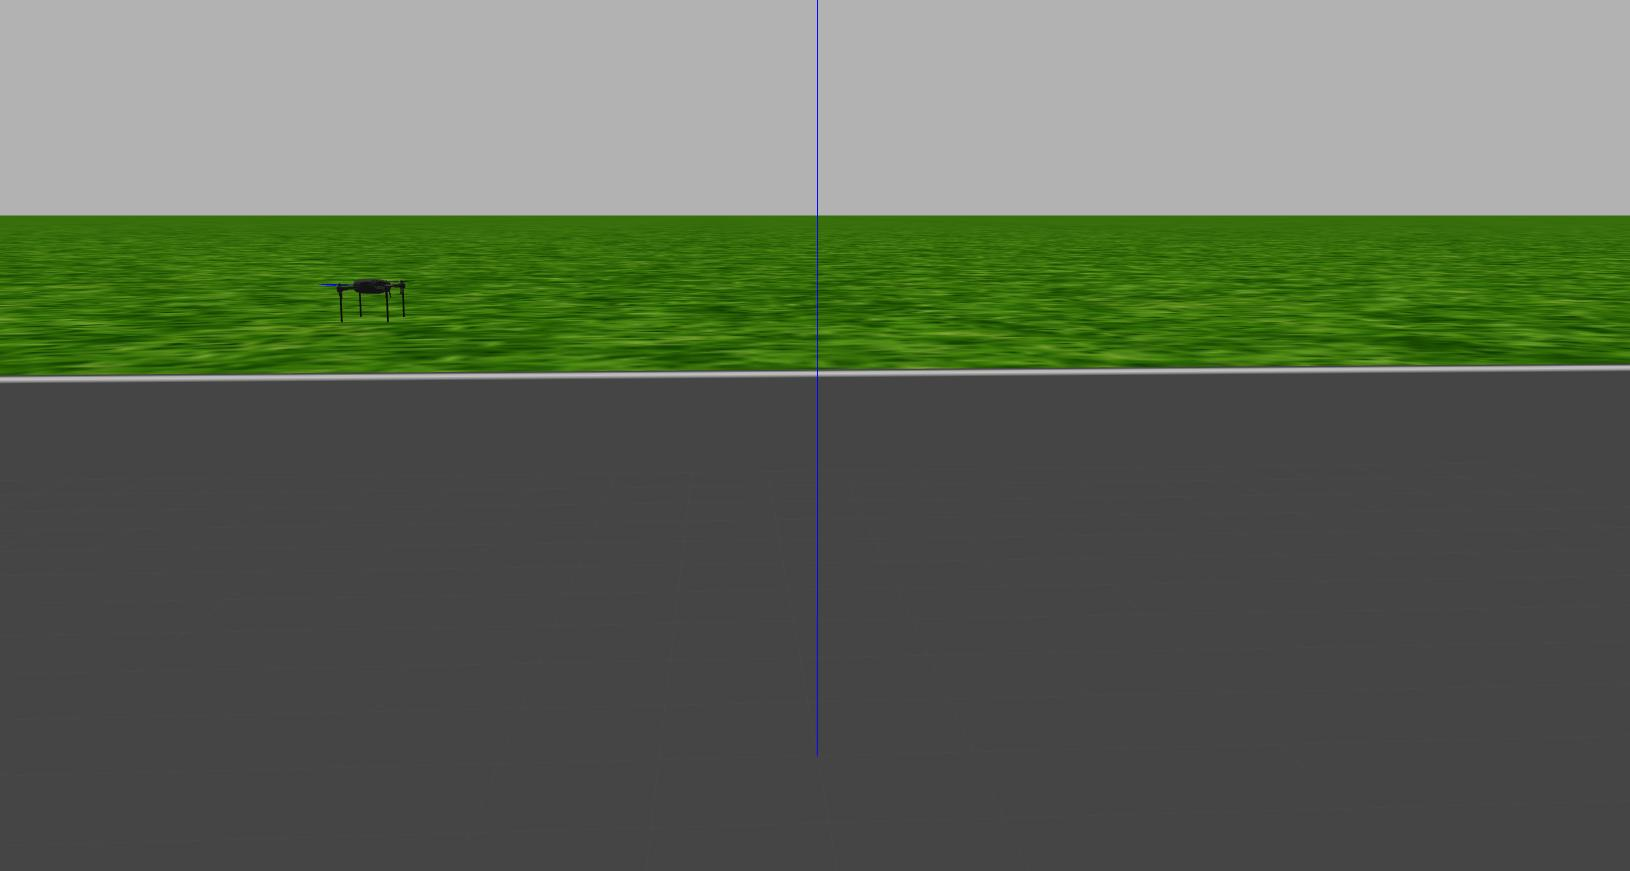
\includegraphics[width=0.48\textwidth]{Ardupilot_sim3.jpg}}}\hfill
    \subfloat[Terminal de ArduPilot lista para recibir comandos de vuelo]{\label{fig:Ardupilot_Ready}{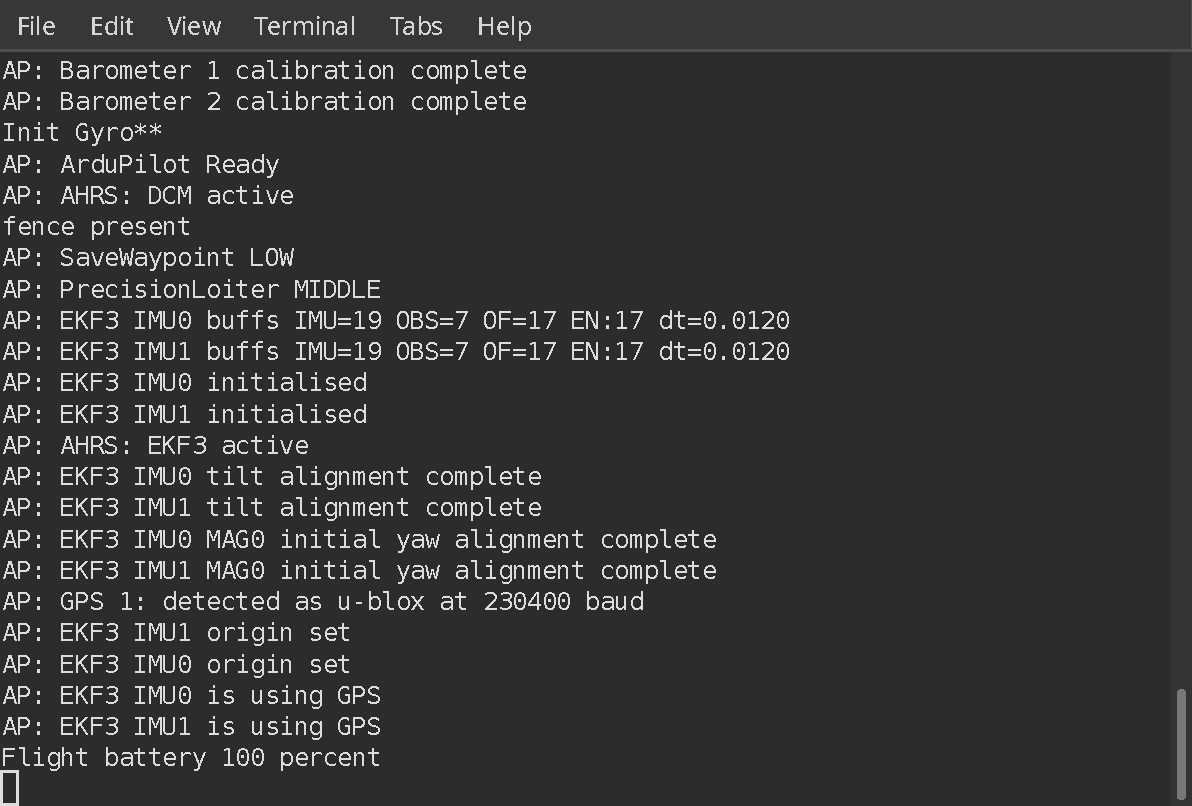
\includegraphics[width=0.48\textwidth]{ArduPilot_Ready.pdf}}}
    \caption{Prueba de integración entre Gazebo y el SIL de ArduPilot}
    \label{fig:Gazebo_Ardupilot}
\end{figure}

\subsection{Instalación de Pymavlink}
Por último, en cuento a la configuración del sistema, es necesario instalar Pymavlink para entablar la comunicación con el framework SIL de ArduPilot, de tal manera que se puedan enviar instrucciones de modos de vuelo, así como comandos que permitan definir la trayectoria de vuelo del dron, a través de un script en Python sin necesidad de ingresar estas instrucciones directamente en una terminal.

La librería Pymavlink está contenida en un módulo de Python, por lo que su instalación resulta un tanto trivial; sin embargo, cabe destacar que es necesario haber instalado el gestor de paquetes de Python 3 para ejecutar los siguientes comandos:

\begin{enumerate}
    \item Actualizar los repositorios y paqueterías del sistema
    \begin{lstlisting}[language = bash]
        $ sudo apt update && sudo apt -y full-upgrade
    \end{lstlisting} 
    
    \item Instala el módulo que contiene la librería
    \begin{lstlisting}[language = bash]
        $ pip3 install mavproxy
    \end{lstlisting} 
\end{enumerate}

Para verificar la instalación de la librería se puede abrir el intérprete de Python 3 en una terminal y transcribir la siguiente serie de comandos

\begin{lstlisting}[language = bash]
    $ python3
    >>> import pymavlink
    >>> print(pymavlink.__doc__)
\end{lstlisting} 

Al ejecutar lo anterior, se debe de generar una impresión en la terminal de la figura \ref{fig:Pymavlink_ver}.

\begin{figure}[ht]
    \centering
    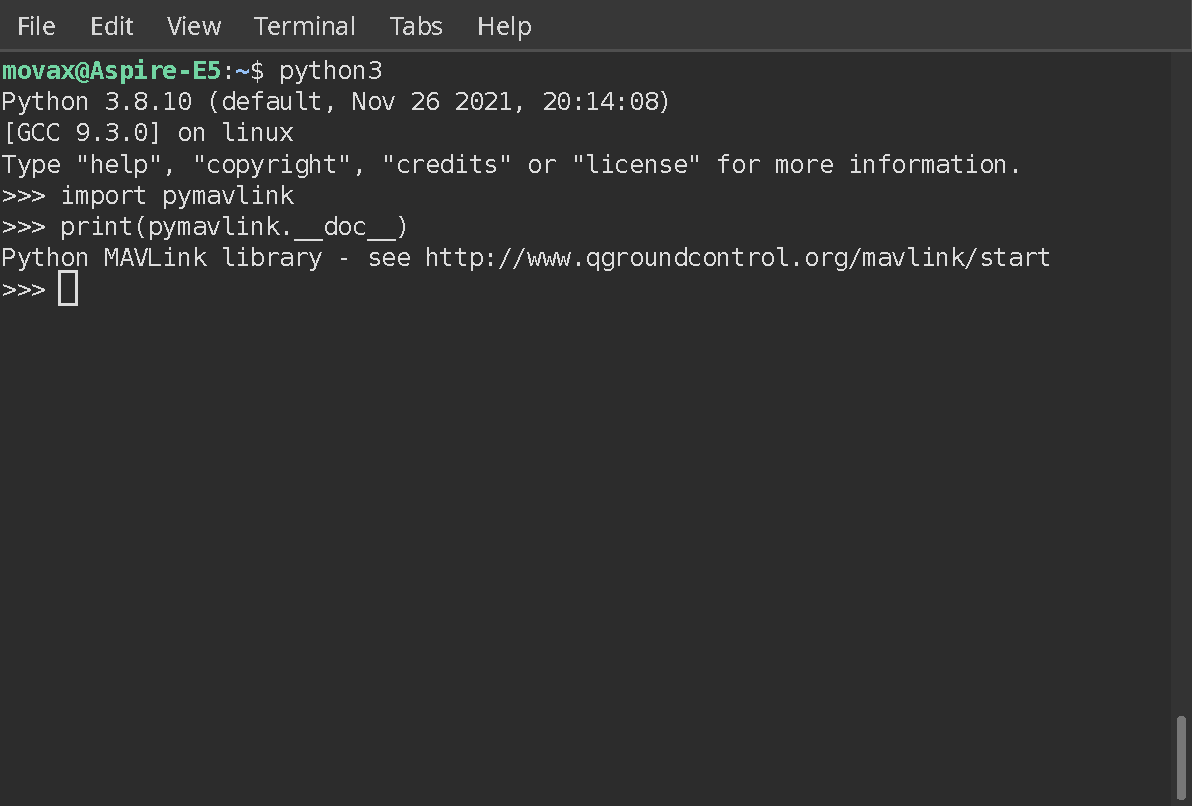
\includegraphics[width=0.7\textwidth]{Pymavlink_ver.pdf}
    \caption{Validación de instalación de Pymavlink}
    \label{fig:Pymavlink_ver}
\end{figure}


\section{Circuito de Vuelo Virtual}
La sección anterior corresponde a la configuración que se realizó para instalar y validar las herramientas que se utilizaron para la elaboración del proyecto. En los siguientes capítulos se detallan el uso específico que se le dio al software instalado, así como las pruebas y los resultados obtenidos; en esta sección se especifica el proceso de elaboración de la simulación con el circuito de vuelo para el dron simulado.

La figura \ref{fig:Circuit} presenta un diagrama con en donde se especifica la estructura del circuito elaborado, en él se pueden apreciar las cotas con las distancias presentes entre cada una de las compuertas, así como el orden del recorrido realizado por el dron. Cabe destacar que el modelo de compuerta que se seleccionó para el circuito de vuelo, fue el utilizado en las distintas competencias del IROS.

\begin{figure}[ht]
    \centering
    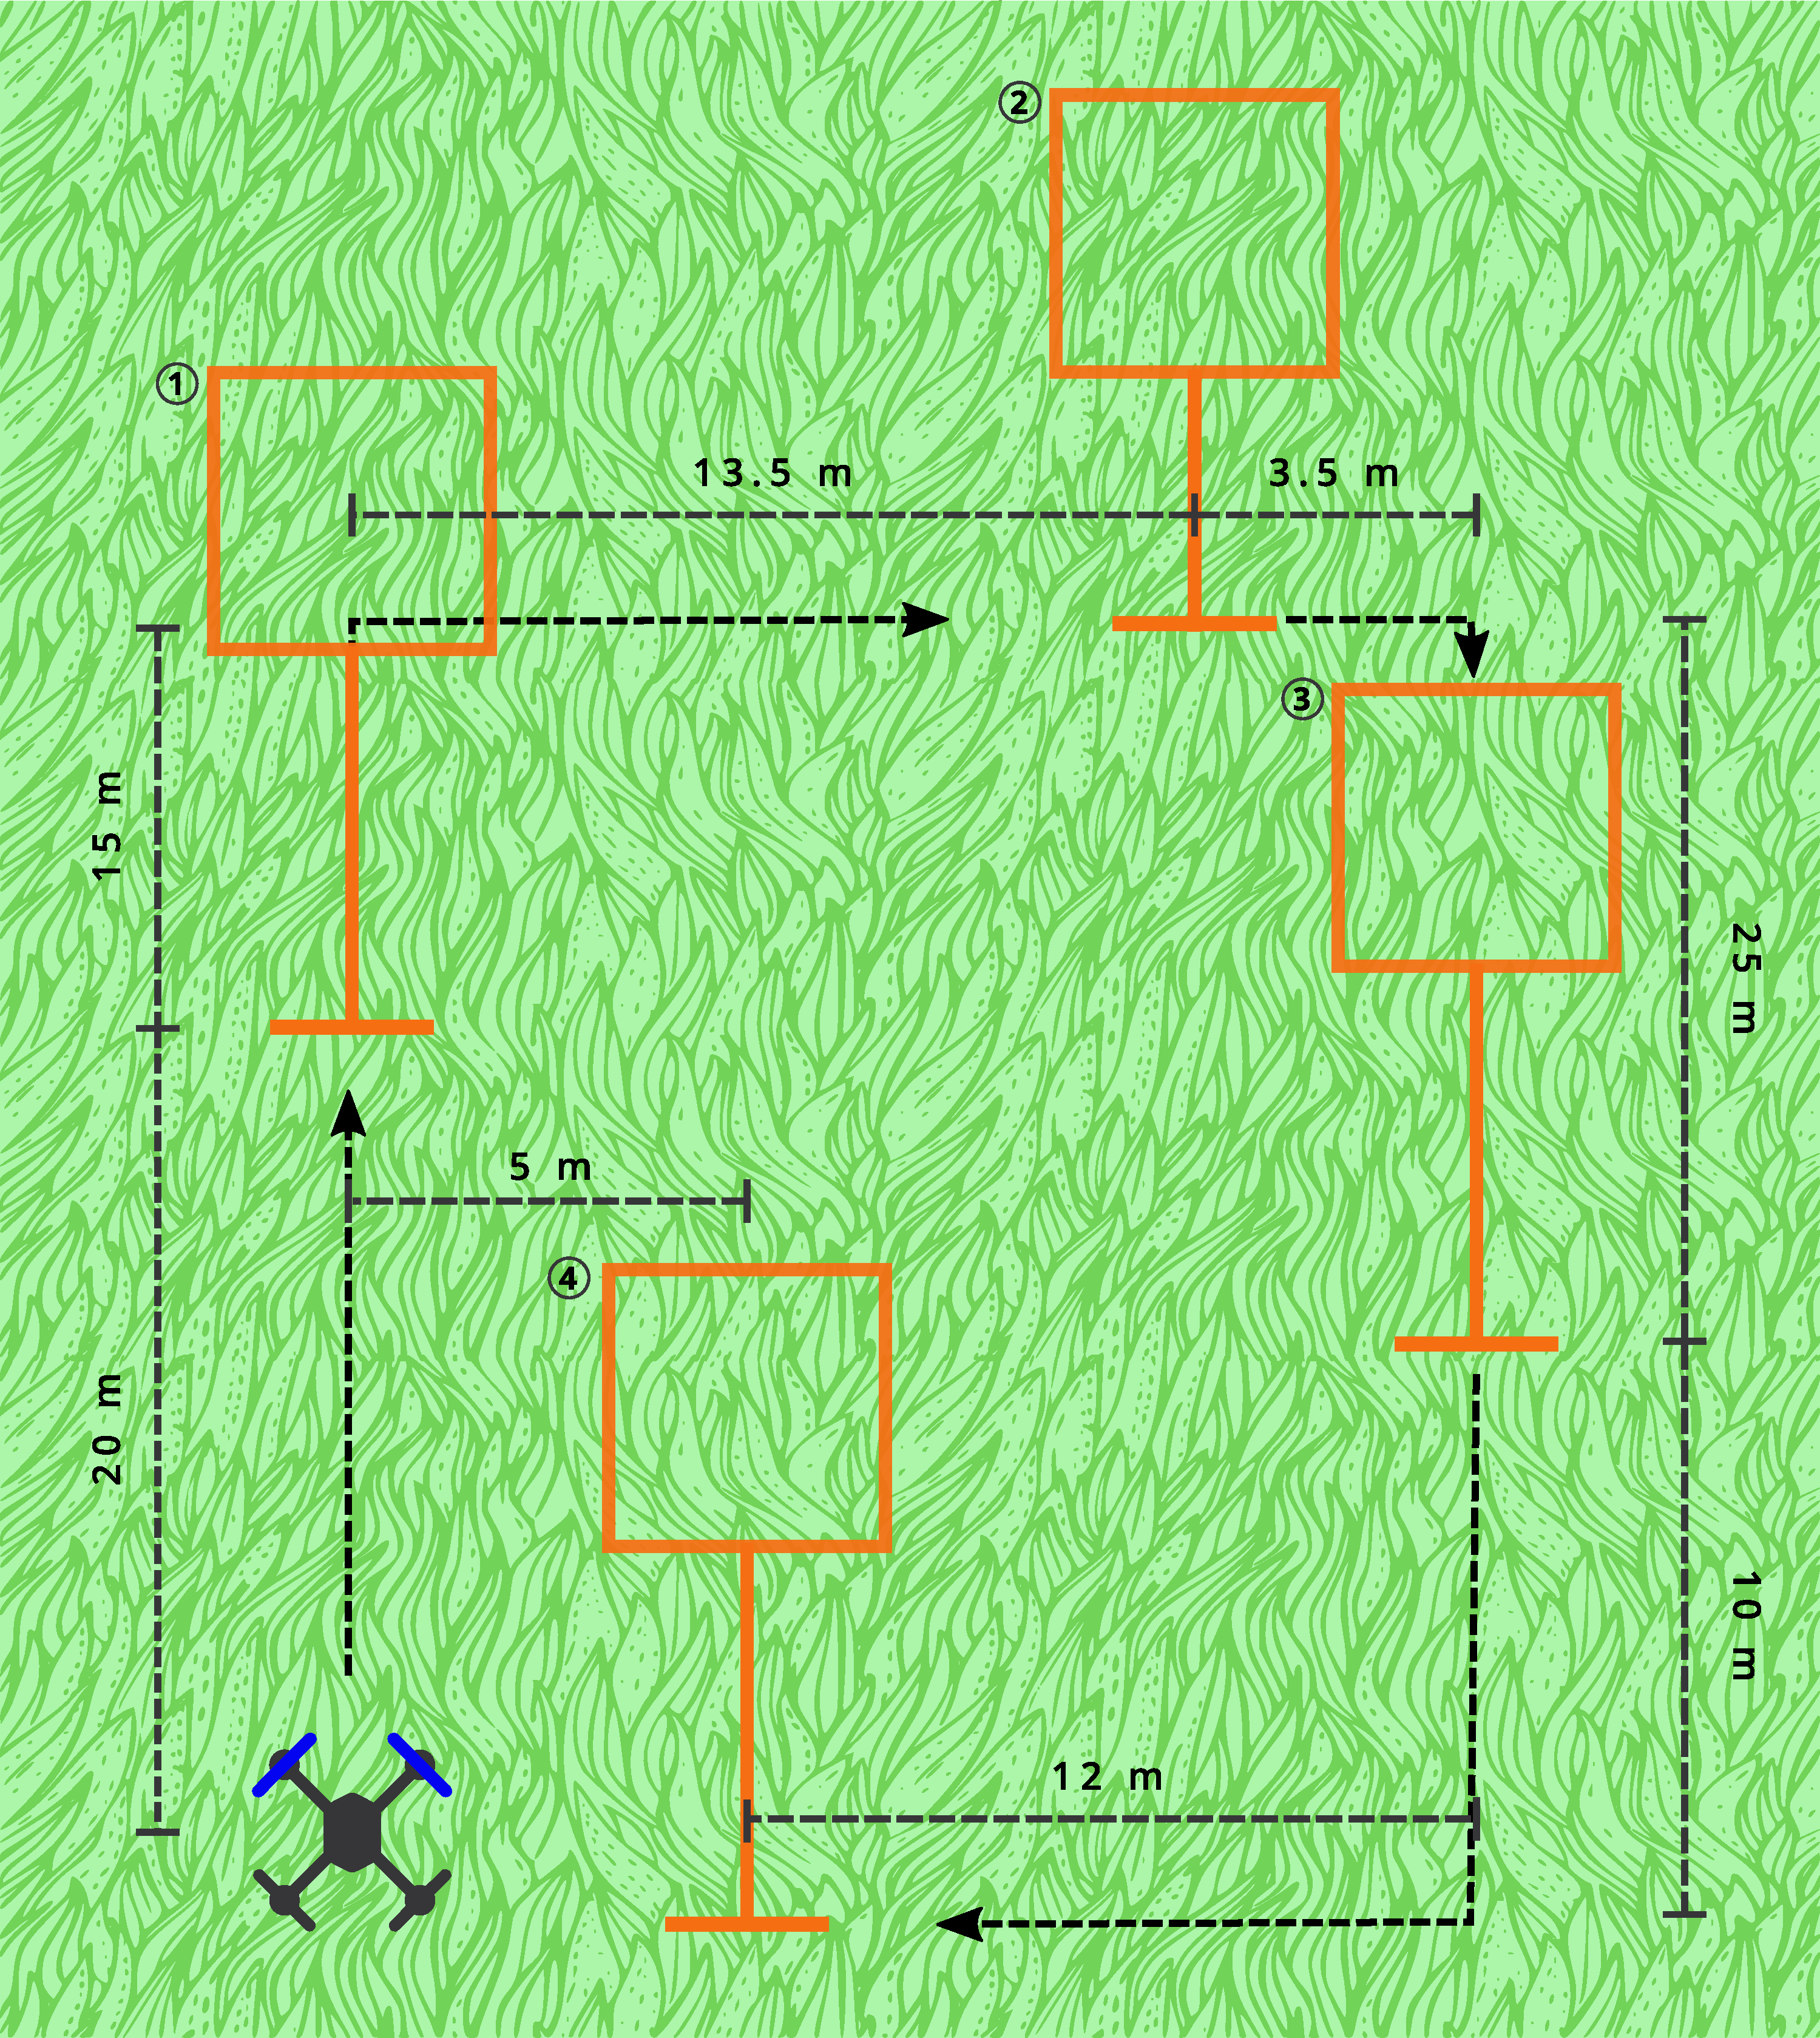
\includegraphics[width=0.8\textwidth]{Circuit.pdf}
    \caption{Esquema detallado del circuito de vuelo elaborado en simulación.}
    \label{fig:Circuit}
\end{figure}

A partir del esquema antes mencionado, la elaboración del circuito dentro de la simulación se llevó a cabo utilizando algunos modelos ya elaborados por la comunidad de Gazebo. Para el terreno y el modelo de la compuerta se utilizaron los modelos elaborados por \cite{rojas2020deeppilot}, los cuales fueron usados para entrenar su red neuronal profunda. Por otro lado, el modelo del dron Iris fue provisto por

Por otro lado, existe un bug al utilizar Gazebo, pues al crear mundo nuevo, no es posible guarda el proyecto con los cambios realizados, el menú de diálogo que aparece la opción de guarda proyecto simplemente no se muestra de forma correcta, por lo que crear un proyecto nuevo resulta imposible de esta forma. Debido o a lo anterior, en este trabajo se propone una solución para sobrellevar el problema anterior; para que el menú se muestre de forma correcta es necesario ejecutar Gazebo con permisos de administrador; sin embargo, al utilizar privilegios de administrador para crear el archivo del proyecto, este se encontrará protegido contra escritura, y resulta muy poco práctico necesitar permisos de administrador para realizar modificaciones sobre el proyecto.

Entonces, para solucionar este segundo problema se debe de crear un archivo utilizando el comando \textit{touch} con la extensión \textit{.world}. Lo anterior genera un archivo un proyecto de Gazebo completamente vacío. Ahora, debido a que este tipo de archivos solamente contiene la descripción de los componentes utilizados en determinado proyecto, así como sus características físicas como posición, es posible abrir el archivo del proyecto con cualquier editor de texto y ver su contenido. Por lo tanto, se puede copiar el contenido del proyecto creado con privilegios de administrador y pegarlo dentro del nuevo proyecto vacío que se acaba de crear.

Hecho lo anterior, lo que queda es eliminar el proyecto protegido contra escritura. Para ello es necesario abrir una terminal dentro del directorio donde se encuentra el proyecto y ejecutar el comando \textit{rm} con permisos de administrador. A continuación se anexa un ejemplo:

\begin{lstlisting}[language = bash]
    $ sudo rm proyectName.world
\end{lstlisting} 

La figura \ref{fig:Gazebo_gates} muestra los modelos 3D utilizados para la elaboración de la simulación; como se mencionó, se ocuparon dos tamaños de compuerta y por lo tanto dos modelos.

Adicionalmente, la figura \ref{fig:Gazebo_iris} presenta el modelo 3D del dron iris utilizado. Cabe destacar que la principal diferencia entre el modelo provisto por \cite{IQ} y el modelo incluido en la simulación de demostración del plugin de Ardupilot para Gazebo, es la orientación de la cámara. En la simulación de demostración, la cámara se encuentra apuntando hacia el suelo, mientras que en el modelo mostrado en la figura, apunta hacía al frente de la dirección de vuelo del dron.

\begin{figure}[ht]
    \centering
    \subfloat[Vista frontal del modelo de compuerta grande]{\label{fig:Gazebo_gate1}{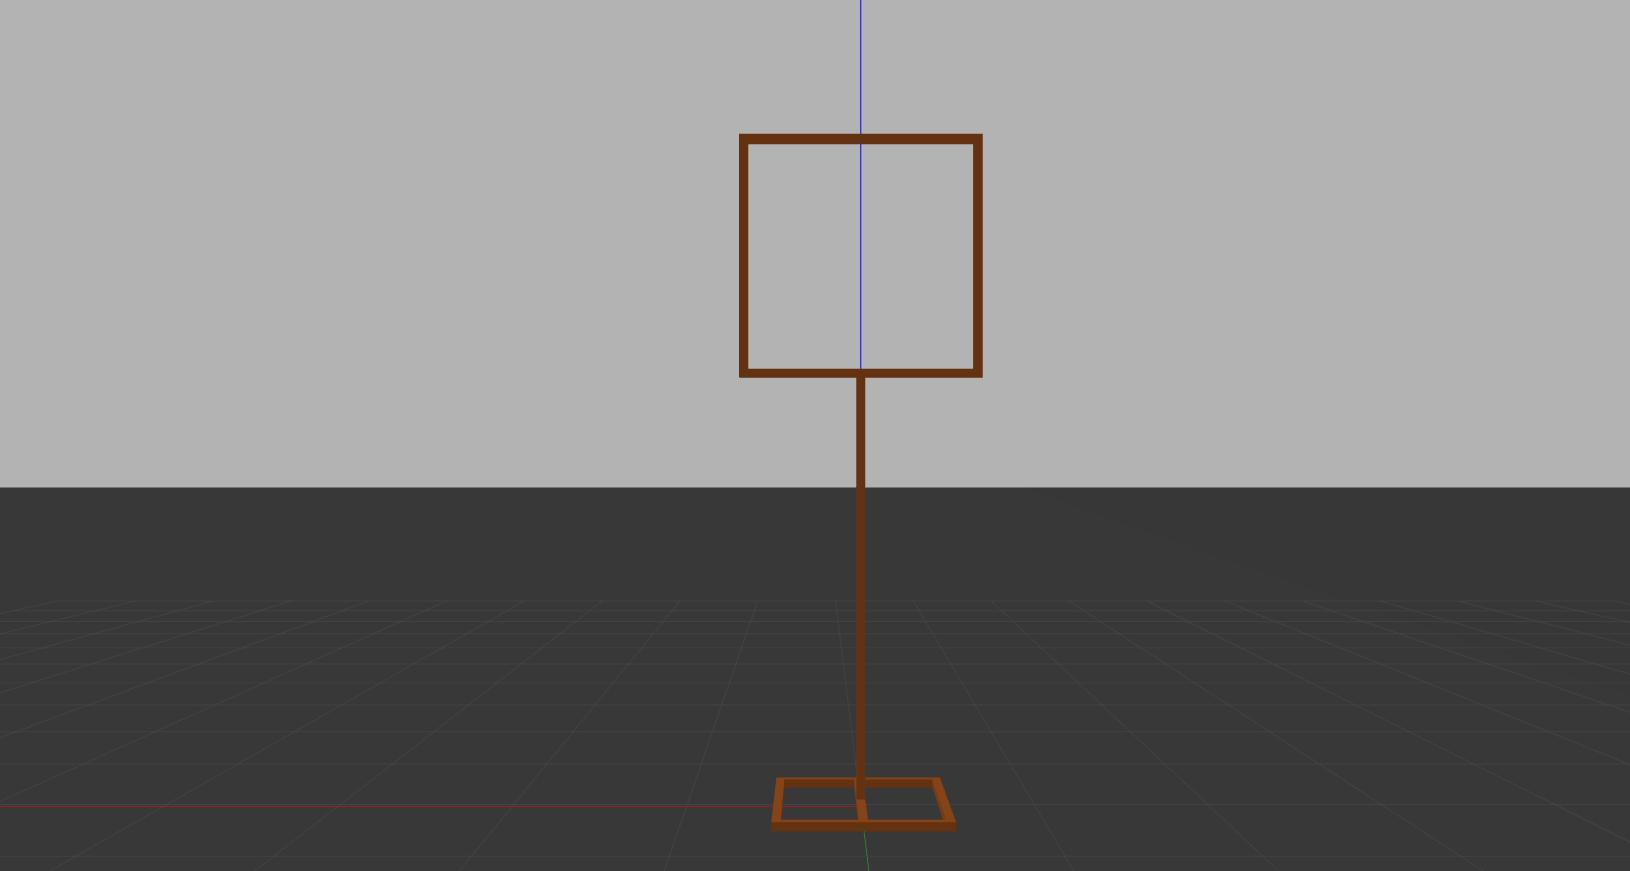
\includegraphics[width=0.48\textwidth]{Gazebo_gate1.jpg}}}\hfill
    \subfloat[Vista superior del modelo de compuerta grande]{\label{fig:Gazebo_gate2}{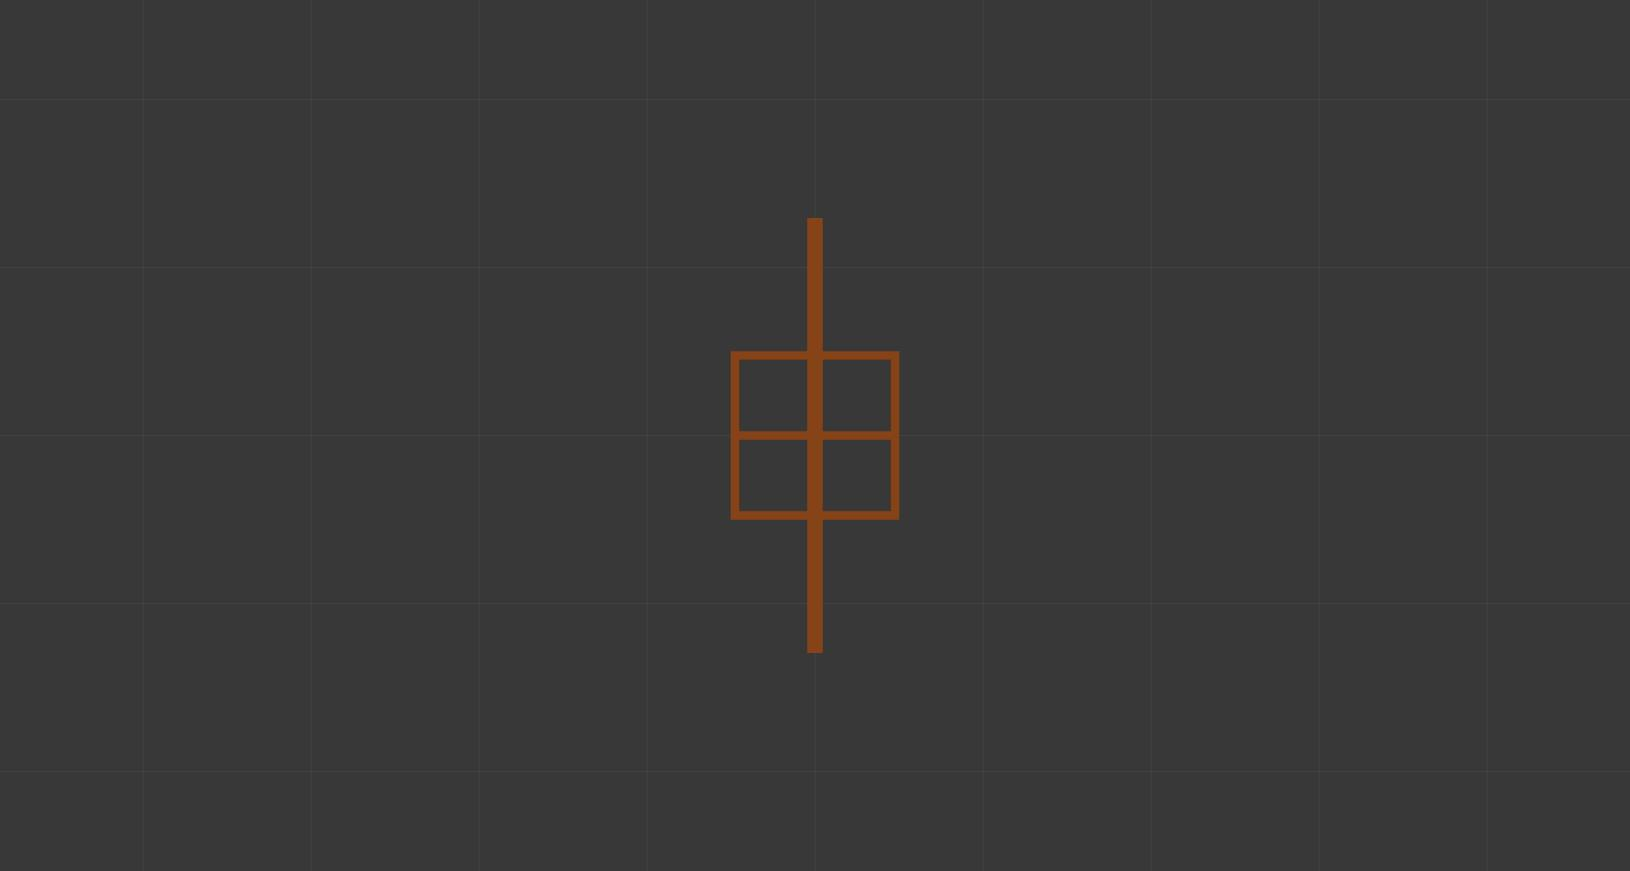
\includegraphics[width=0.48\textwidth]{Gazebo_gate2.jpg}}}\\
    \subfloat[Vista frontal del modelo de compuerta mediana]{\label{fig:Gazebo_gate3}{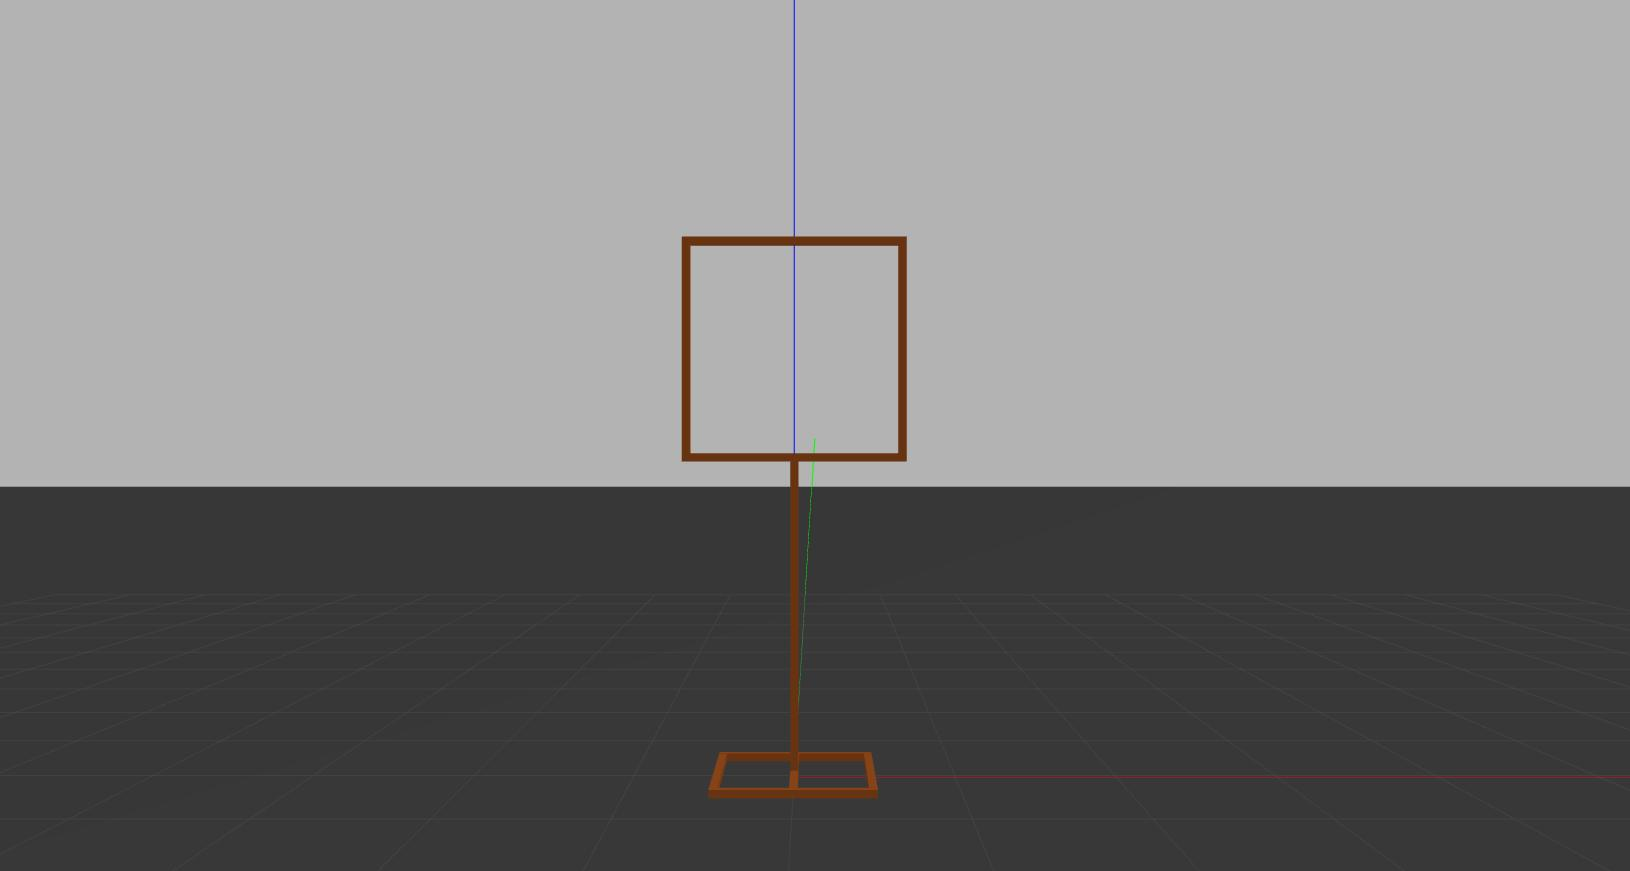
\includegraphics[width=0.48\textwidth]{Gazebo_gate3.jpg}}}\hfill
    \subfloat[Vista superior del modelo de compuerta mediana]{\label{fig:Gazebo_gate4}{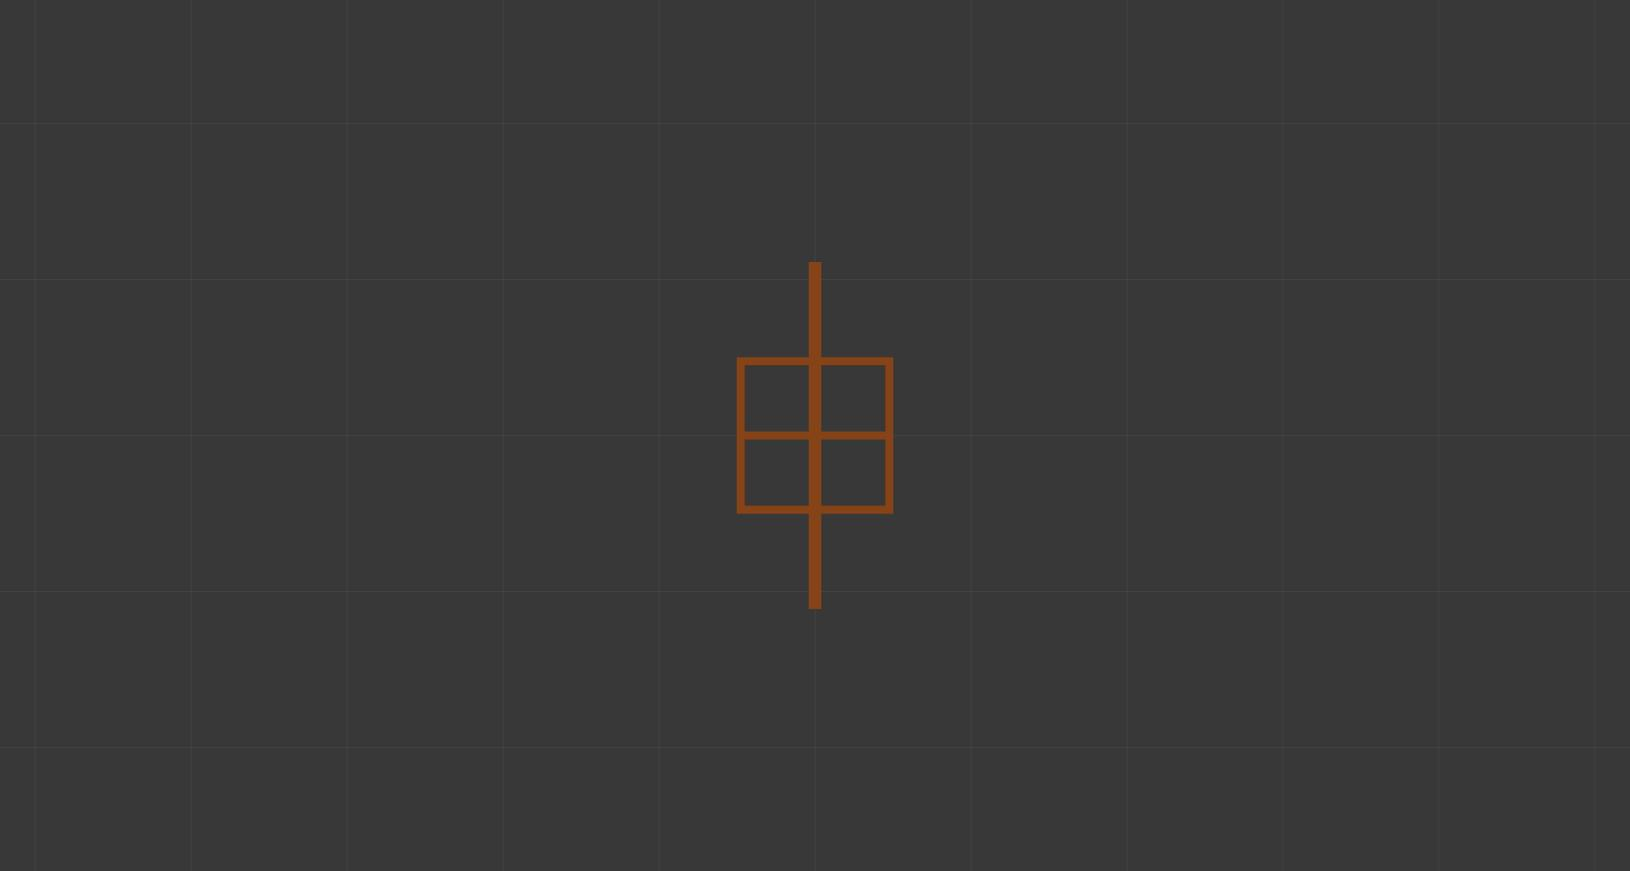
\includegraphics[width=0.48\textwidth]{Gazebo_gate4.jpg}}}
    \caption{Modelos de compuerta proveídos por \cite{rojas2020deeppilot}}
    \label{fig:Gazebo_gates}
\end{figure}

\begin{figure}[ht]
    \centering
    \subfloat[Vista trasera]{\label{fig:Gazebo_iris1}{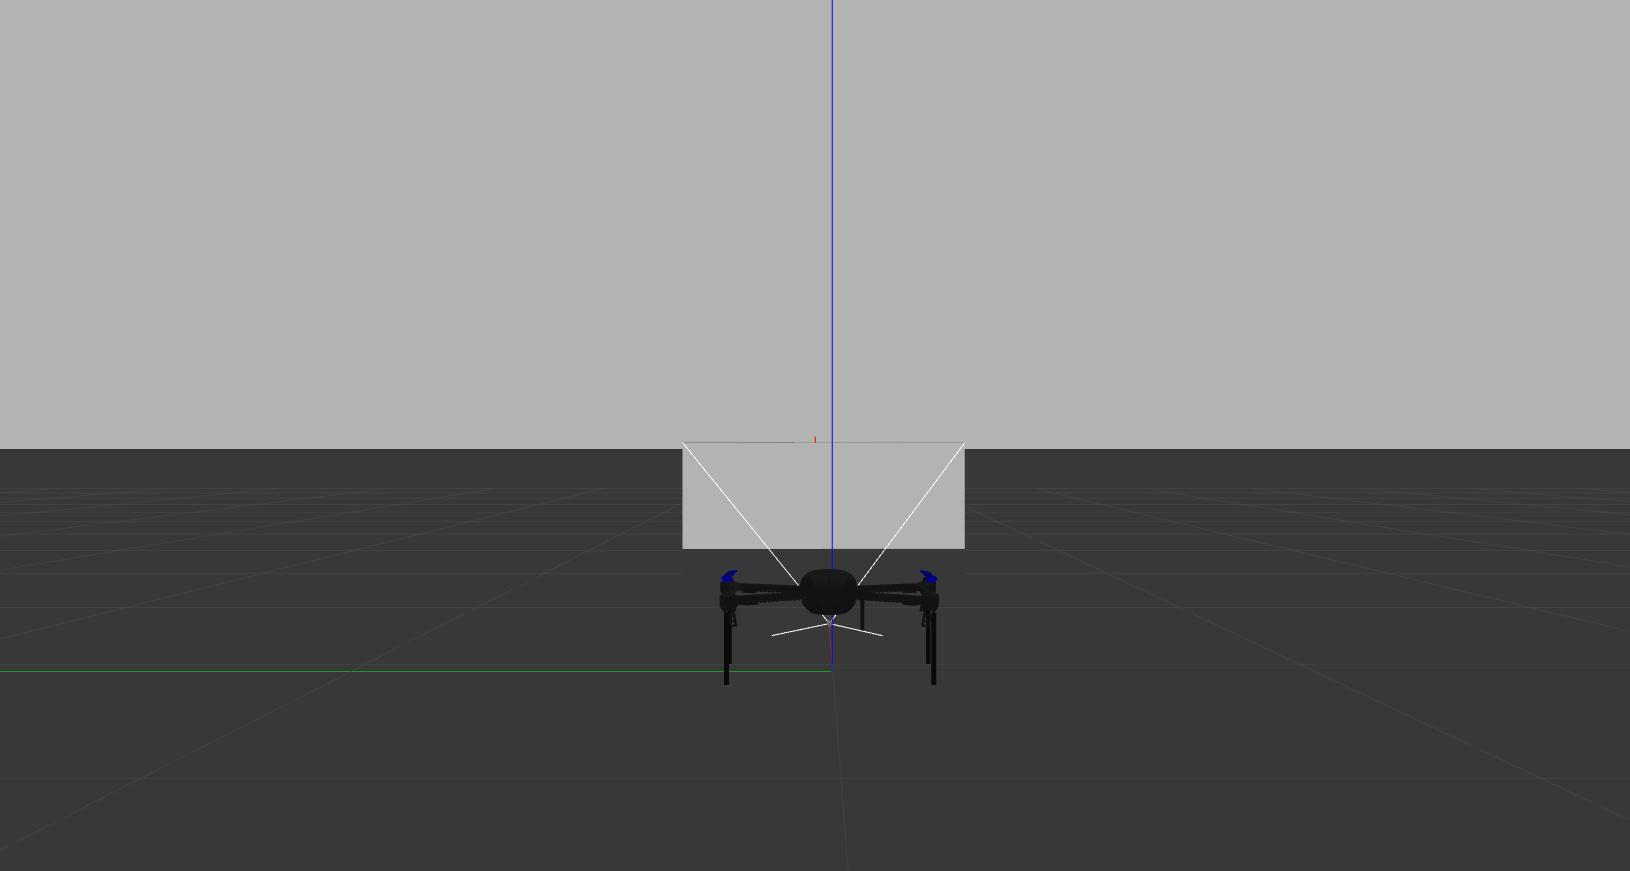
\includegraphics[width=0.48\textwidth]{Gazebo_iris1.jpg}}}\hfill
    \subfloat[Vista lateral]{\label{fig:Gazebo_iris2}{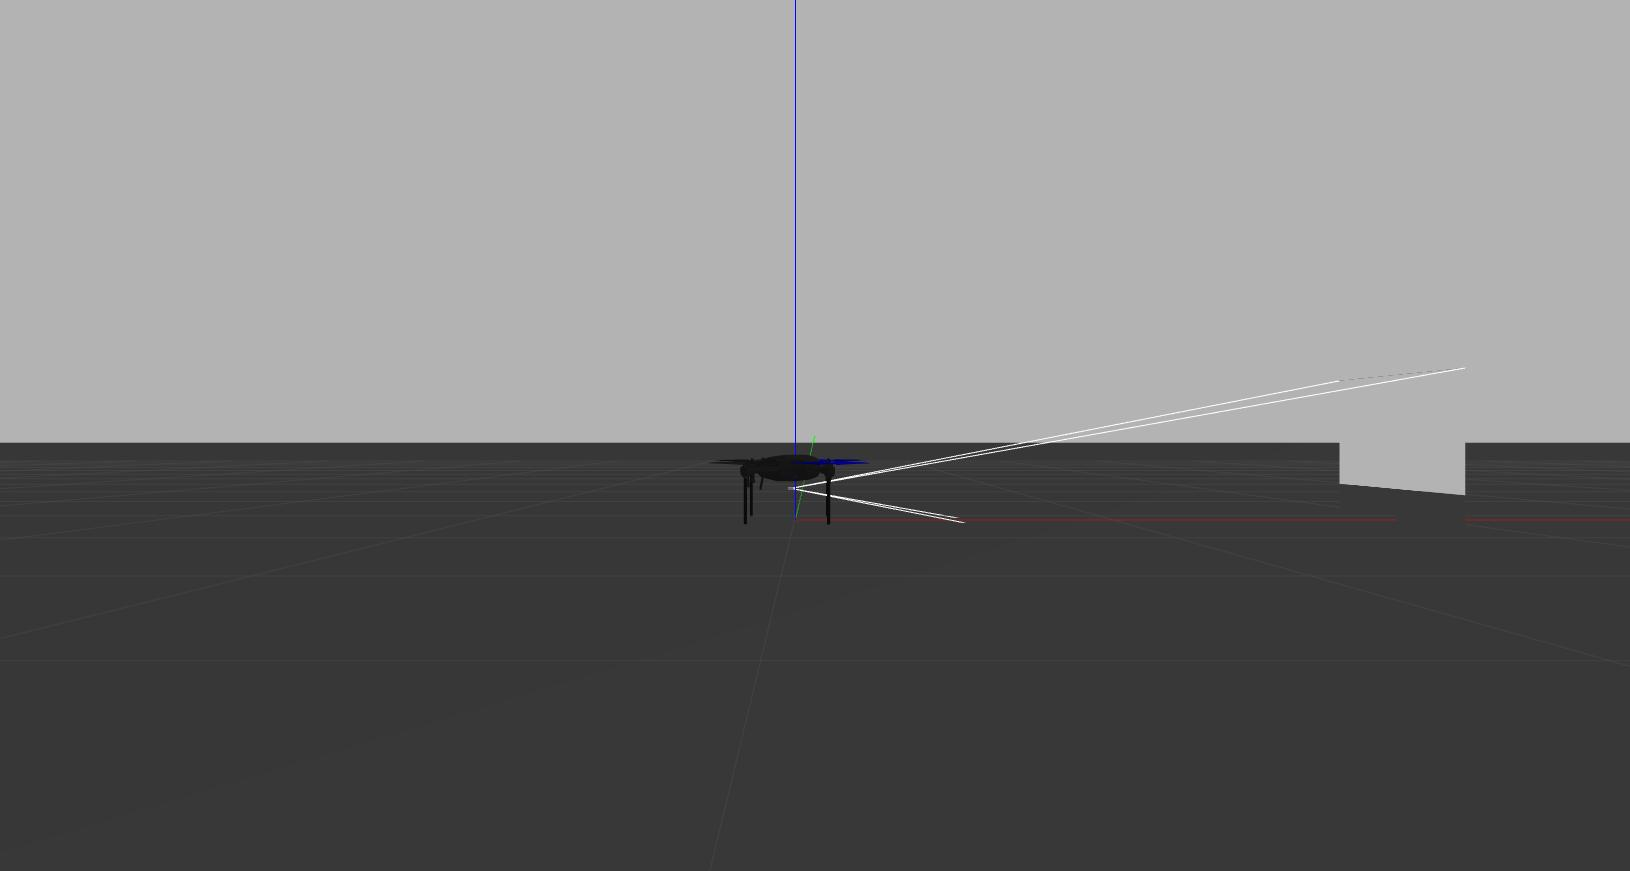
\includegraphics[width=0.48\textwidth]{Gazebo_iris2.jpg}}}\\
    \subfloat[Vista superior]{\label{fig:Gazebo_iris3}{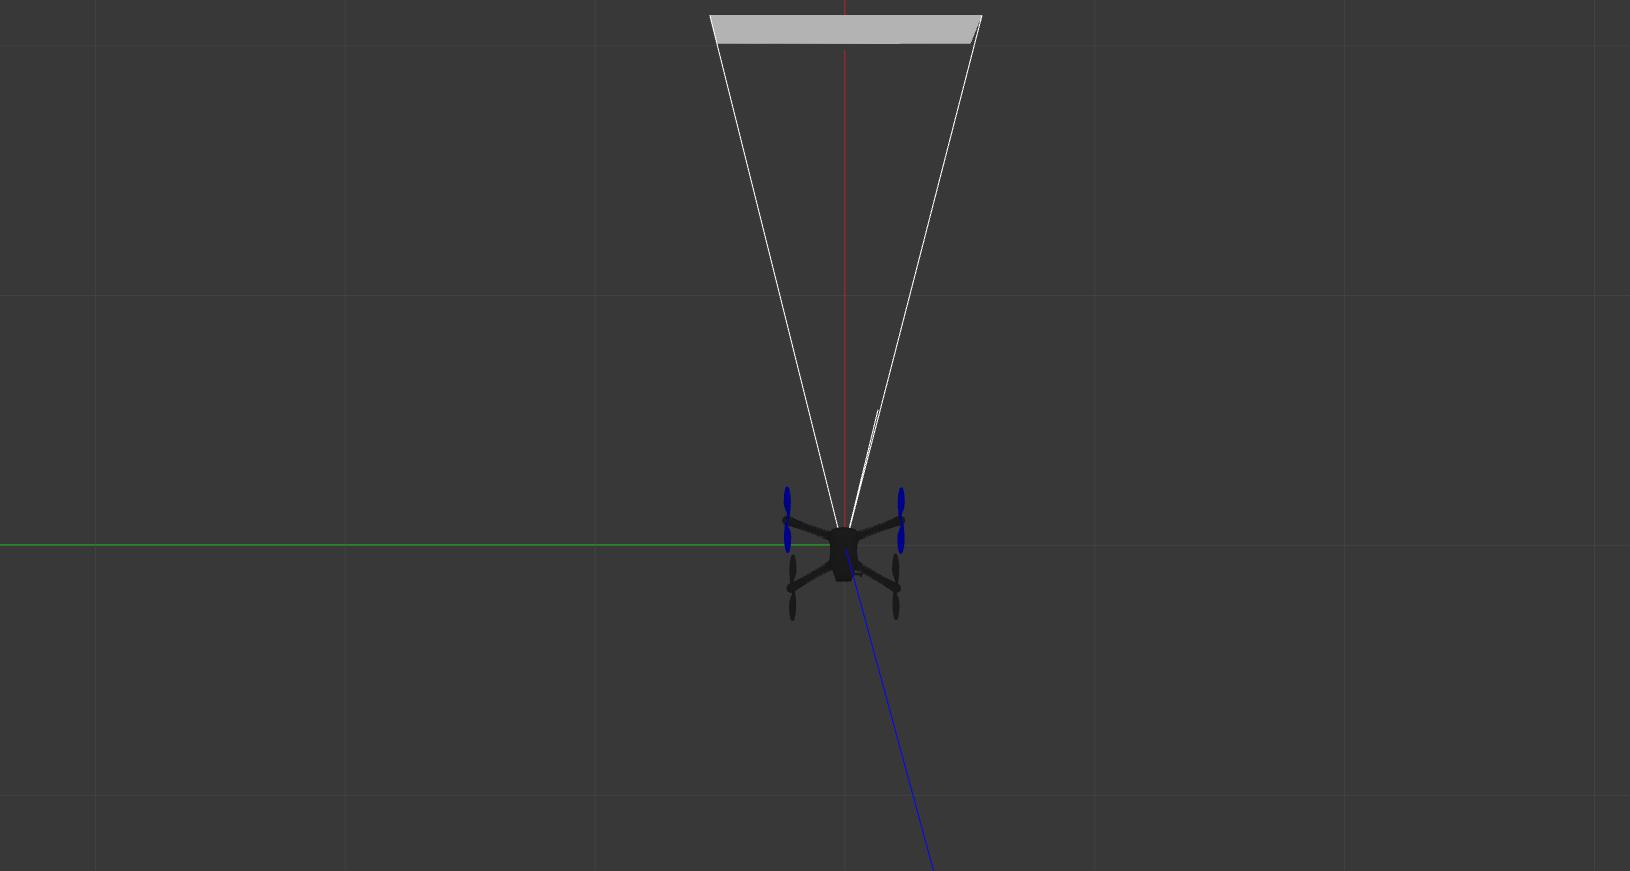
\includegraphics[width=0.48\textwidth]{Gazebo_iris3.jpg}}}\hfill

    \caption{Modelo de dron iris con cámara frontal provisto por \citet{IQ}}
    \label{fig:Gazebo_iris}
\end{figure}


Por último, la figura \ref{fig:Gazebo_worlds} muestra algunas capturas tomadas dentro del proyecto creado para implementar el circuito de vuelo implementado. La figura \ref{fig:Gazebo_world1} presenta un panorama general del circuito de vuelo, en ella se observan las cuatro compuertas del circuito, el dron iris y el modelo de un edificio; este último se incluyó para fines del algoritmo de visión artificial. Por otro lado, las figura \ref{fig:Gazebo_world2} y \ref{fig:Gazebo_world3}  muestran otras perspectivas del circuito y de los objetos que lo componen. Finalmente, la figura \ref{fig:Gazebo_world4} muestra la perspectiva del dron Iris junto con la toma captada por la cámara simulada en este.

\begin{figure}[ht]
    \centering
    \subfloat[]{\label{fig:Gazebo_world1}{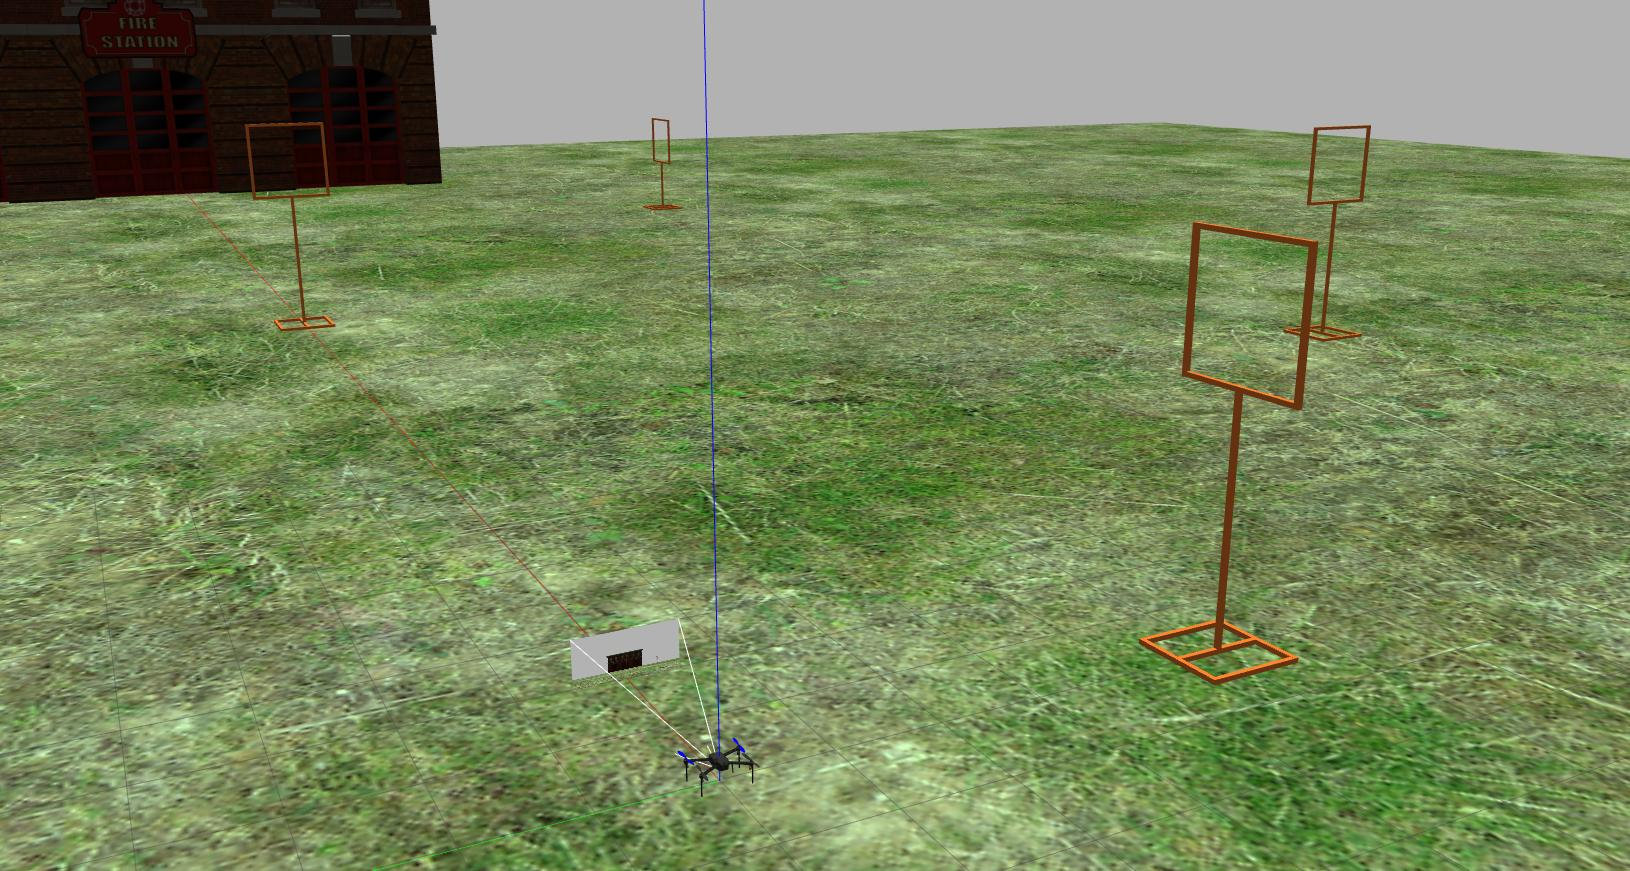
\includegraphics[width=0.48\textwidth]{Gazebo_world1.jpg}}}\hfill
    \subfloat[]{\label{fig:Gazebo_world2}{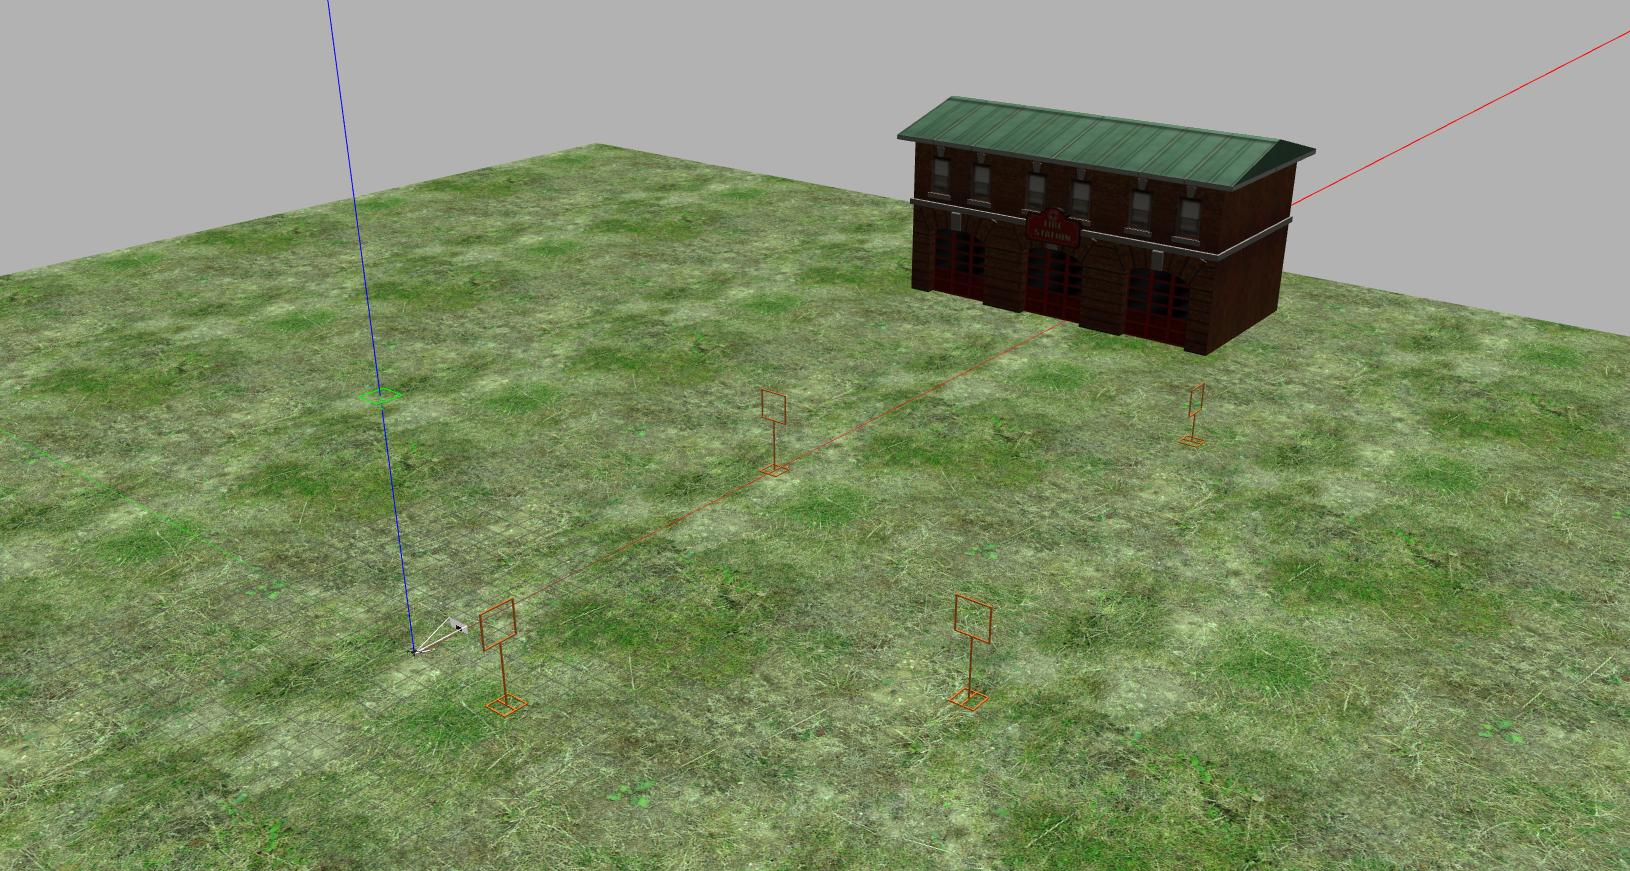
\includegraphics[width=0.48\textwidth]{Gazebo_world2.jpg}}}\\
    \subfloat[]{\label{fig:Gazebo_world3}{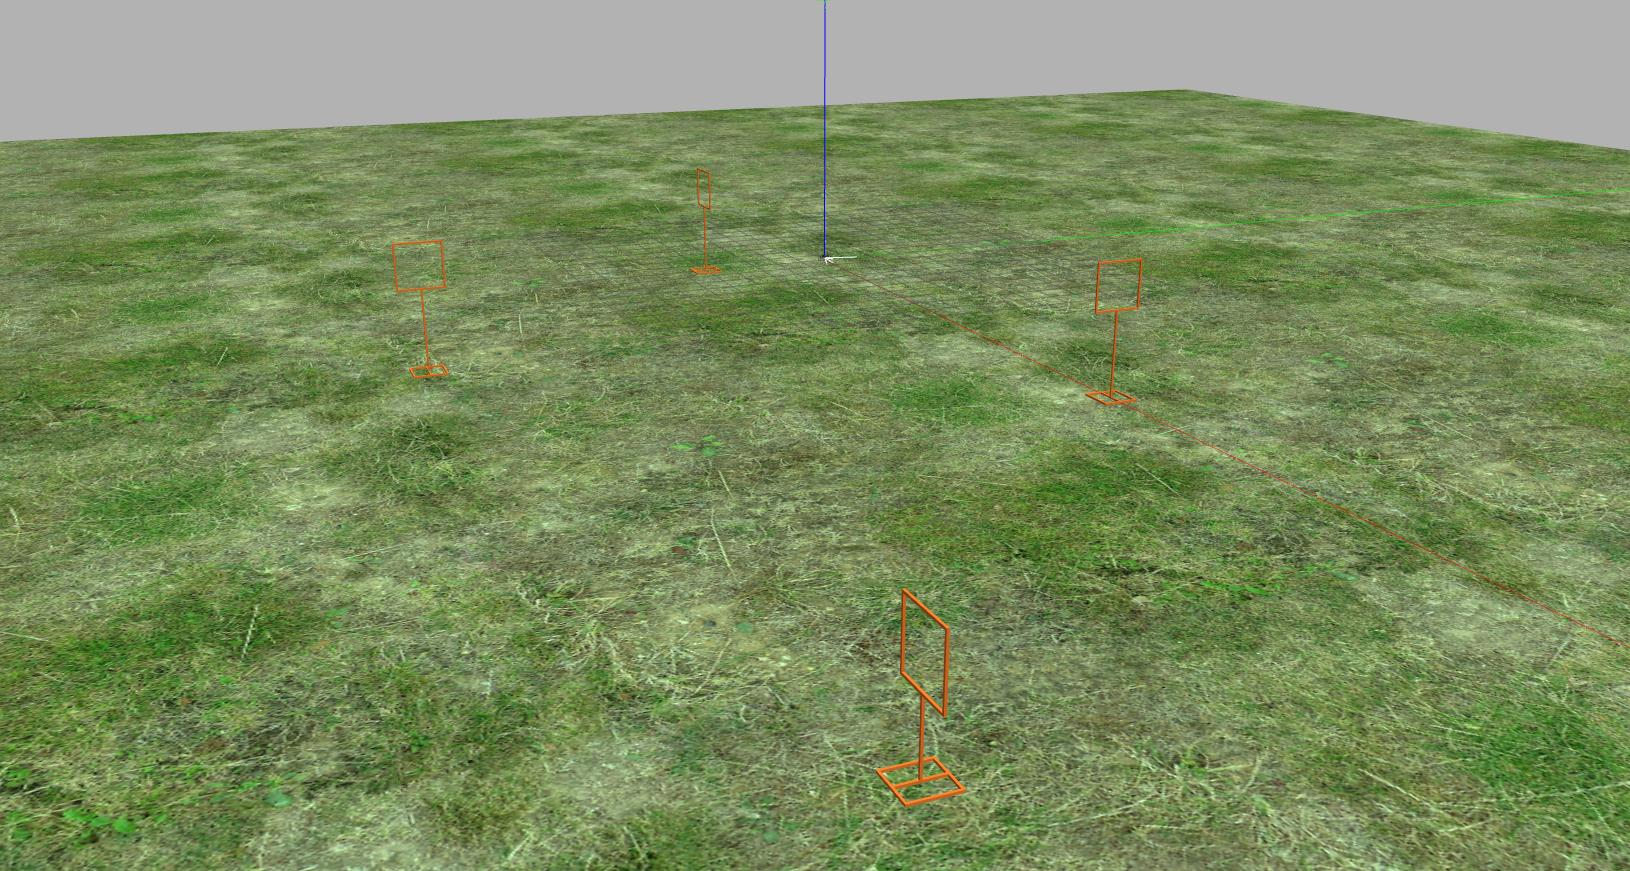
\includegraphics[width=0.48\textwidth]{Gazebo_world3.jpg}}}\hfill
    \subfloat[]{\label{fig:Gazebo_world4}{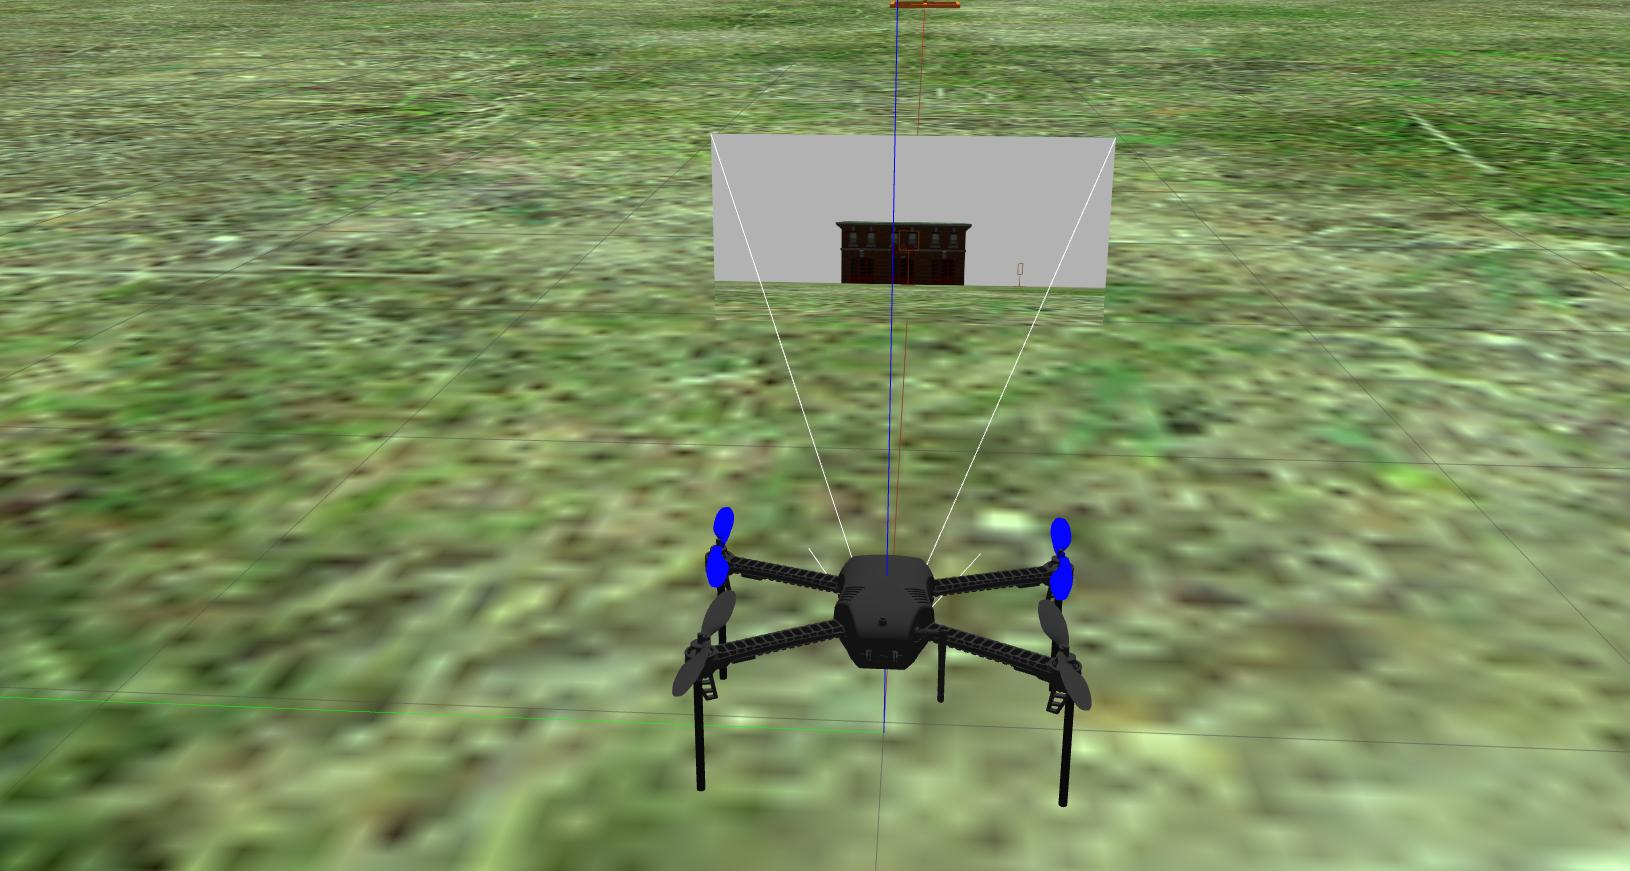
\includegraphics[width=0.48\textwidth]{Gazebo_world4.jpg}}}\hfill

    \caption{Capturas del ambiente de simulación implementado}
    \label{fig:Gazebo_worlds}
\end{figure}


\chapter{Validación del algoritmo de visión artificial}


\section{Descripción del sistema y forma de trabajo}
En esta sección se describe el procedimiento realizado para llevar a cabo la adecuación del algoritmo de visión artificial para la detección de compuertas dentro del circuito de vuelo. Cabe mencionar que, como se mostró en la sección anterior, el tipo de compuertas seleccionadas para la formación del circuito de vuelo fue un modelo similar al utilizado en las competencias del IROS, con un característico color naranja. Ahora bien, debido a que el algoritmo de visión artificial está basado en la detección de color y no utiliza redes neuronales el aspecto más importante para adecuar el algoritmo es encontrar el rango de color en la escala HSV para nuestro objeto, o mejor dicho el color de nuestro objeto.

Entonces, para lograr sintonizar lo mejor posible la escala de color, se utilizó como base un rango de color adecuado para detectar el color naranja, pues este es el color principal del objeto de interés; sin embargo, el color de las compuertas es una de la infinidad de tonalidades derivadas del naranja, por lo que fue necesario ajustar más el rango para que, de ser posible, el algoritmo fuera capaz de detectar exclusivamente las compuertas y no diera falsos positivos con objetos con una tonalidad derivada del naranja. Por otro lado, dentro del circuito de vuelo el único objeto con una tonalidad similar al color naranja es el edificio que se encuentra detrás de la primera compuerta, por lo que, se están asumiendo condiciones prácticamente ideales para la detección de las compuertas.

Dicho lo anterior, la figura \ref{fig:cv_hsv} corresponde al mapa de color utilizado para definir el rango base para el algoritmo de detección. El diagrama está compuesto por 3 partes; el eje \textit{x} corresponde al rango de valores para el matiz (hue), por otro lado, la primera parte del eje \textit{y}, denotado con un (1), pertenece a los valores de matiz con una saturación que varía entre 0 y 255, así mismo, la segunda parte del eje \textit{y}, identificada con un (2), denota los valores de matiz para los cuales los coeficientes de saturación y valor son iguales a 255. Entonces, para obtener la escala para la detección de un color, se debe escoger el valor de matiz y saturación correspondiente, y posteriormente establecer el coeficiente de valor entre 25 y 255.

Por lo tanto, a partir de la figura \ref{fig:cv_hsv} la escala base seleccionada para la detección del color naranja fue: \[H:5-25;\text{ } S:75-255;\text{ } V:25-255\]

\begin{figure}[ht]
    \centering
    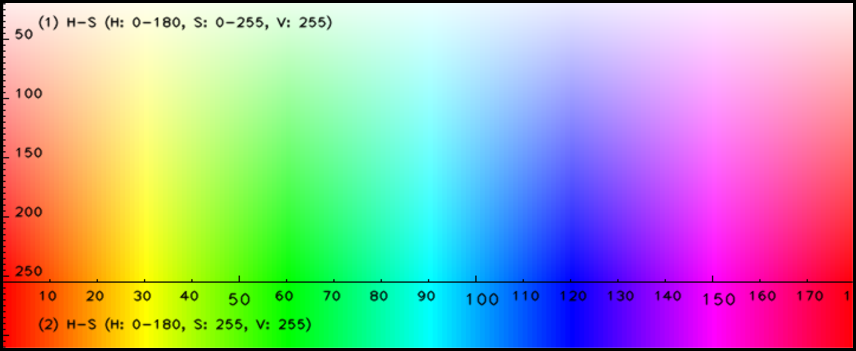
\includegraphics[width=0.8\textwidth]{cv_hsv.pdf}
    \caption{Mapa de color en escala HSV \cite{dey_2020}}
    \label{fig:cv_hsv}
\end{figure}

\section{Sintonización de la escala de color}

La sub-sección anterior representa el argumento para la selección de la escala inicial, ahora bien, como se mencionó al inicio de esta sección, fue necesario ajustar el rango de color para proveer al algoritmo de mayor precisión y robustez al momento de detectar las compuertas del circuito de vuelo. Lo anterior se logró utilizando imágenes del ambiente de simulación, de tal manera que se aplicó una máscara con el rango de color especificado y se fueron variando los valores de las componentes del modelo de color hasta observar que el algoritmo aislaba de manera satisfactoria las compuertas del resto de objetos en el circuito. La figura \ref{fig:cv_gates} muestra las imágenes utilizadas con este fin. La figura \ref{fig:cv_gate1} corresponde a una fotografía obtenida a partir de la cámara simulada a bordo del dron, se trata de un primer plano hecho a una de las compuertas del circuito de vuelo, además, la figura \ref{fig:cv_gate2} corresponde a una toma captada en tercera persona, en donde hay dos compuertas visibles y el dron intenta cruzar a través de una de ellas, incluso puede notarse el fotograma captado por la cámara del dron. Por otro lado, la figura \ref{fig:cv_gate3} presenta otra toma en tercera persona, en donde es visible una compuerta y el dron se encuentra estático en el suelo, en esta fotografía se destaca el uso de un ambiente diferente al ambiente construido para el circuito de vuelo; por último, la figura \ref{fig:cv_gate4} presenta una toma del circuito de vuelo en donde se alzan a apreciar dos compuertas y el único edificio incluido en el ambiente de simulación. 

Cabe destacar que  con las figuras \ref{fig:cv_gate3} y \ref{fig:cv_gate4} se buscó darle mayor robustez al algoritmo de detección de compuertas, utilizando otro tipo de ambiente y objetos de otros colores para realizar una calibración más adecuada del rango de color utilizado.

A partir de lo ya mencionado, para realizar la sintonización del rango de color se elaboró un script de Python, en donde se hizo uso de OpenCV para cargar las imágenes mostradas en la figura \ref{fig:cv_gates}, convertir su modelo de color de BGR a HSV, y posteriormente ejecutar el algoritmo de detección con la escala de color base. Lo anterior se realizó de manera individual con cada una de las imágenes, de tal manera que con cada una se ajustó la escala base de forma gradual hasta observar una detección aceptable; es decir, hasta que la detección eliminara la mayor cantidad de falsos positivos en la imagen, dejando solamente las siluetas de las compuertas. 

Es importante mencionar que en este punto del desarrollo del trabajo, el algoritmo no se encontraba ejecutándose de forma indefinida en algún proceso, sino que, se ejecuta una sola vez sobre cada imagen, por lo que lo único que se necesitó para realizar la sintonización fueron las imágenes en cuestión para realizar el ajuste; es decir, el script elaborado no requiere de la ejecución del ambiente creado en Gazebo o de una instancia del SITL de ArduPilot para realizar el ajuste de la escala, este funciona de forma independiente. El proceso seguido para ejecutar el algoritmo desde un nodo en ROS se describe más adelante, en su respectiva sección.


\begin{figure}[ht]
    \centering
    \subfloat[]{\label{fig:cv_gate1}{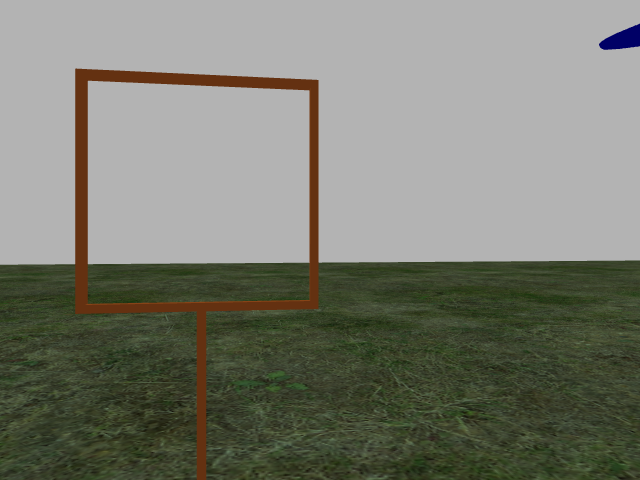
\includegraphics[width=0.48\textwidth]{Gate.png}}}\hfill
    \subfloat[]{\label{fig:cv_gate2}{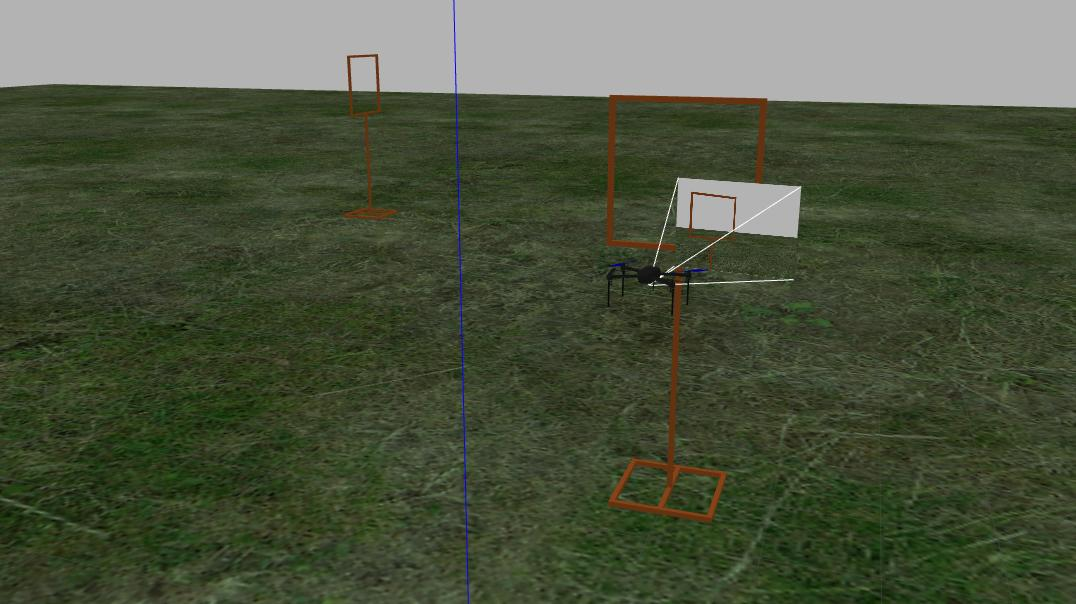
\includegraphics[width=0.48\textwidth]{Gate2.jpg}}}\\
    \subfloat[]{\label{fig:cv_gate3}{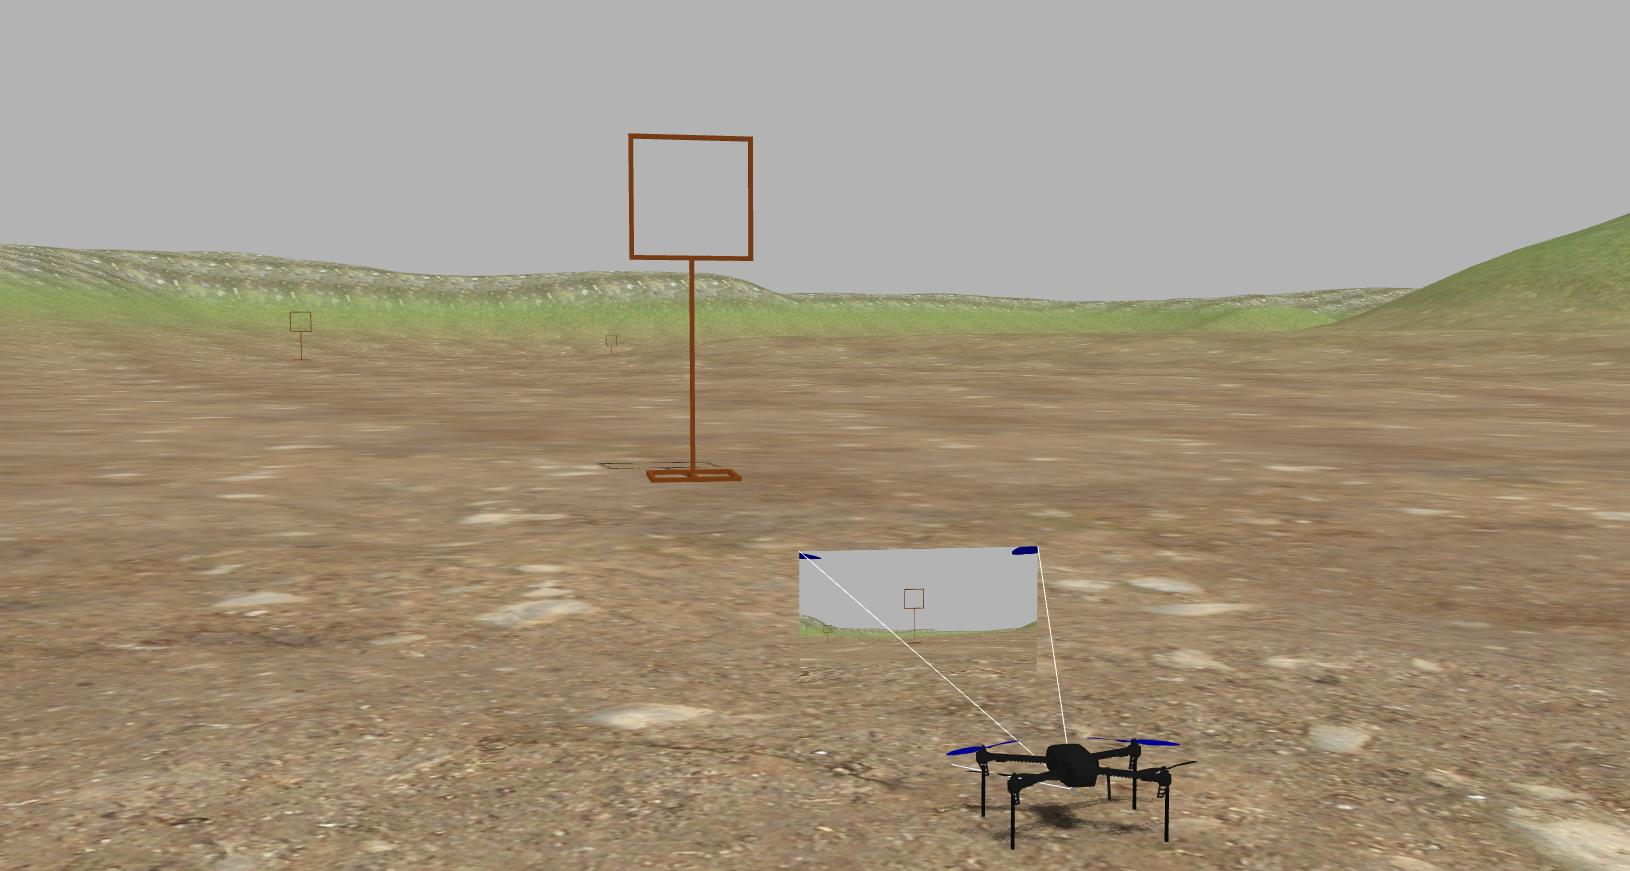
\includegraphics[width=0.48\textwidth]{Gate3.jpg}}}\hfill
    \subfloat[]{\label{fig:cv_gate4}{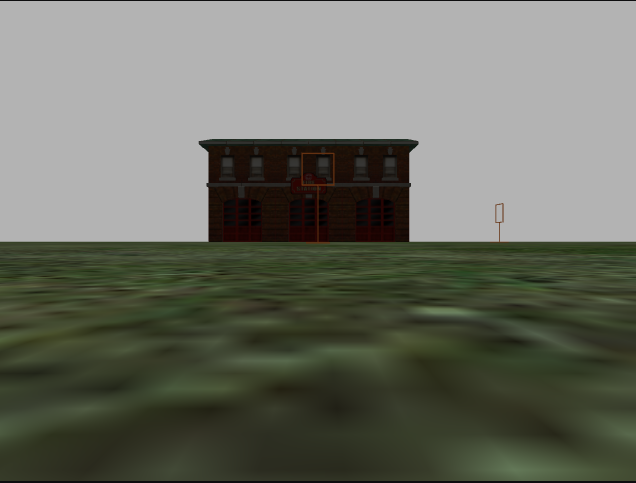
\includegraphics[width=0.48\textwidth]{Gate4.png}}}\hfill

    \caption{Imágenes utilizadas para la sintonización del rango de color}
    \label{fig:cv_gates}
\end{figure}

Entonces, a partir de la escala base se realizó la primera prueba del algoritmo de detección sobre la colección de imágenes. La figura \ref{fig:cv_gatesth1} muestra los resultados obtenidos en esta prueba. Tomando en cuenta el contexto anterior, la figura \ref{fig:cv_gate1th1} muestra la detección efectuada en la imagen en primer plano de una de las compuertas, como se puede observar, la detección es prácticamente perfecta y se logra aislar con gran precisión la compuerta del fondo, el suelo y el fragmento visible de pala de uno de los rotores del dron. A manera de secuencia, la figura \ref{fig:cv_gate2th1} presenta la fotografía en tercera persona de las dos compuertas, se aprecia que se logra aislar de gran manera el control de las compuertas, dejando a un lado el suelo y el dron;  sin embargo, el algoritmo no es capaz de detectar el fragmento de compuerta que se observa en la previsualización de la toma de la cámara del dron. Después, la figura \ref{fig:cv_gate3th1} presenta el comportamiento que se presentó sobre la imagen con cambio de ambiente, es posible observar que en este caso la detección es menos exacta, pues si bien es posible apreciar el aislamiento de gran parte del contorno de la compuerta, el suelo del ambiente también forma parte de la detección, pues su tonalidad entra en el rango de color de la escala base. Por último, la figura \ref{fig:cv_gate4th1},presenta el efecto de la detección sobre la imagen con el edificio del ambiente de simulación en el fondo, en esta primera prueba, está último caso presenta el peor desempeño por parte del algoritmo de detección, pues no fue capaz de captar en absoluto las compuertas de la imagen, sino que, más bien aisló la fachada rojiza del edificio; estos dos últimos casos son un claro ejemplo del porqué fue necesario realizar ajustes en el rango de color utilizado.


\begin{figure}[ht]
    \centering
    \subfloat[]{\label{fig:cv_gate1th1}{
\includegraphics[width=0.48\textwidth]{Gate1_TH1.png}}}\hfill
    \subfloat[]{\label{fig:cv_gate2th1}{
\includegraphics[width=0.48\textwidth]{Gate2_TH1.png}}}\\
    \subfloat[]{\label{fig:cv_gate3th1}{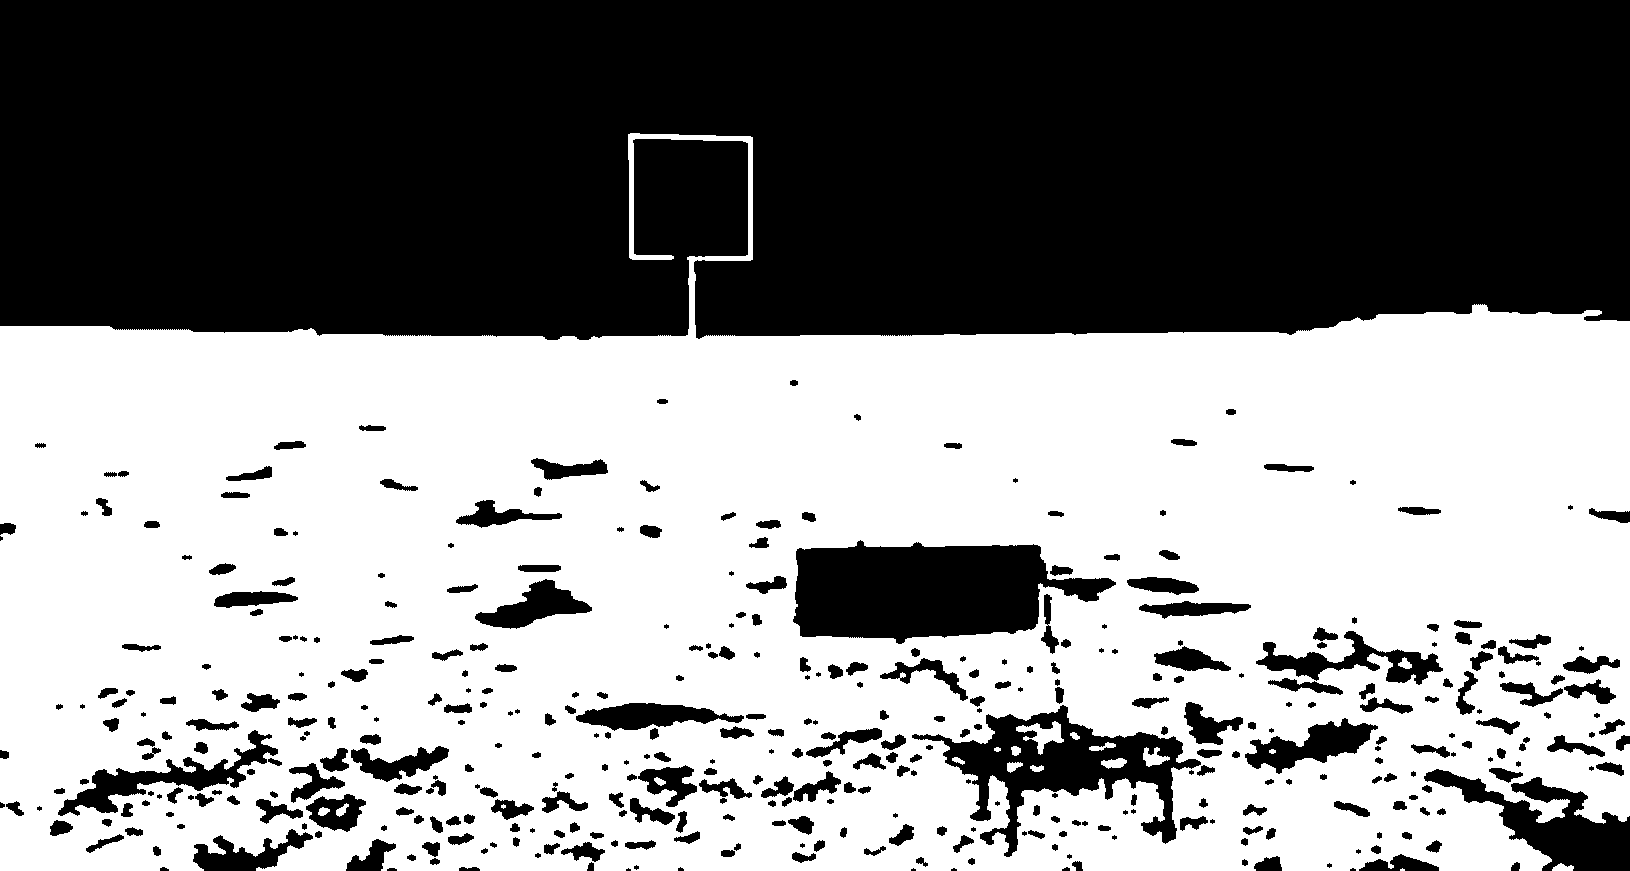
\includegraphics[width=0.48\textwidth]{Gate3_TH1.png}}}\hfill
    \subfloat[]{\label{fig:cv_gate4th1}{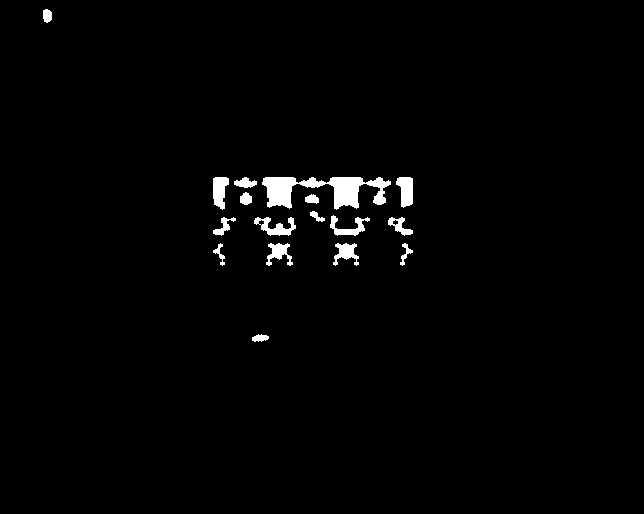
\includegraphics[width=0.48\textwidth]{Gate4_TH1.png}}}\hfill

    \caption{Detección de compuerta con el primer rango de color}
    \label{fig:cv_gatesth1}
\end{figure}

Dándole continuidad a lo observado, realizando el ajuste del rango base, se llegó una serie de valores que mejoraron notablemente el desempeño del algoritmo de detección. El proceso para la sintonización fue el ya expresado, de tal manera que se jugó con el límite inferior de cada parámetro en el modelo de color HSV, hasta que se observó una mejora en la detección de cada una de las imágenes, principalmente en las últimas dos, pues son las que presentaron los resultados más paupérrimos en las primeras pruebas. Entonces, el rango de color que se obtuvo con el reajuste es el siguiente: \[H:5-25;\text{ } S:99-255;\text{ } V:77-171\]

Se observa que el rango para el matiz permaneció igual, mientras que los parámetros de saturación y valor percibieron un cambió un tanto significativo. La figura \ref{fig:cv_gatesth2} muestra los resultados obtenidos a partir de sintonización realizada, a grandes rasgos presenta el mismo número de imágenes que en la prueba anterior, y es posible observar que la detección para la figura \ref{fig:cv_gate1th2} y \ref{fig:cv_gate2th2} permaneció prácticamente igual, aun que no del todo. Realmente el desempeño logrado en la figura \ref{fig:cv_gate1th2} fue bastante bueno, por lo que en este caso no se observa ninguna mejora en particular, por otro lado, en cuanto a la figura \ref{fig:cv_gate2th2}, es posible observar que el reajuste provocó la eliminación de algunas secciones de la compuerta más cercana al dron, y en cuento a segunda compuerta de la imagen, se observa una perdida bastante significativa en cuanto a la detección; sin embargo, esto no representa un comportamiento no deseado, del todo, pues tomando en cuenta el objetivo del algoritmo de detección y la ruta de vuelo seguida por el dron, se puede llegar a la conclusión de que realmente en ningún momento del vuelo el dron tendrá en su campo de visión a más de una compuerta a la vez, y si lo llega a hacer, lo que se buscó es que el dron fuera capaz de detectar la compuerta más cercana a él, por lo que las compuertas del fondo pierden cierto grado de relevancia para esta aplicación en particular. 

En contraste con el caso anterior, el desempeño referente a la figura \ref{fig:cv_gate3th2} presenta una gran mejora con respecto a la primera prueba realizada, a tal grado que el porcentaje de falsos positivos obtenidos por la tonalidad del suelo resulta ser mucho menor, y en este caso ya es posible observar en mayor proporción el contorno y superficie de la compuerta. Por otro lado, la detección efectuada en la figura \ref{fig:cv_gate4th2} sigue siendo bastante pobre, y al realizar el reajuste de la escala de color, ya no fue posible detectar ningún objeto dentro de esta imagen, por lo que la imagen resultante se encuentra completamente en negro.


\begin{figure}[ht]
    \centering
    \subfloat[]{\label{fig:cv_gate1th2}{
\includegraphics[width=0.48\textwidth]{Gate1_TH2.png}}}\hfill
    \subfloat[]{\label{fig:cv_gate2th2}{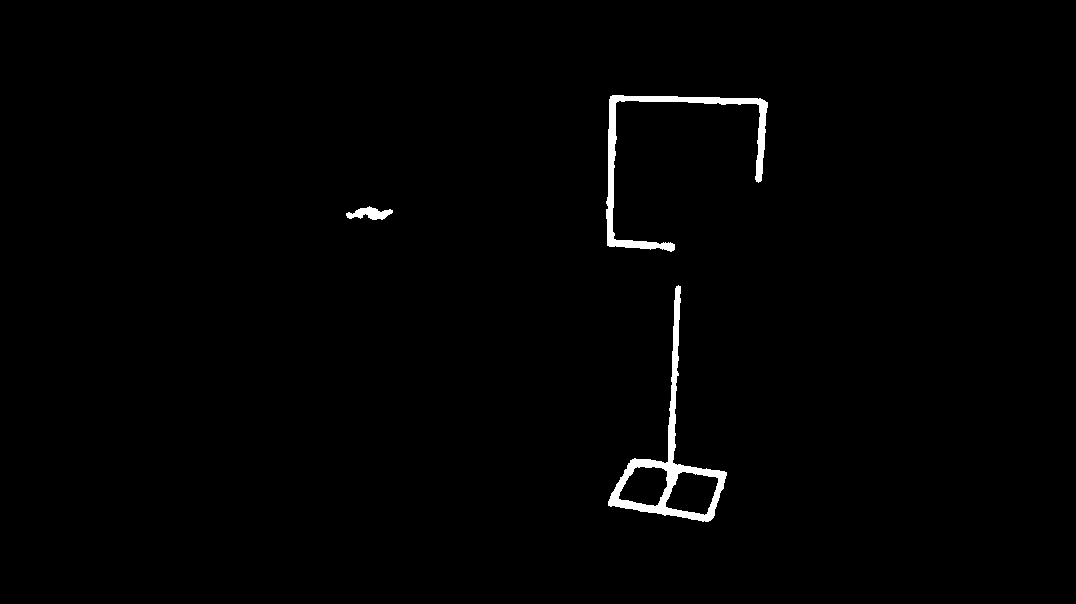
\includegraphics[width=0.48\textwidth]{Gate2_TH2.png}}}\\
    \subfloat[]{\label{fig:cv_gate3th2}{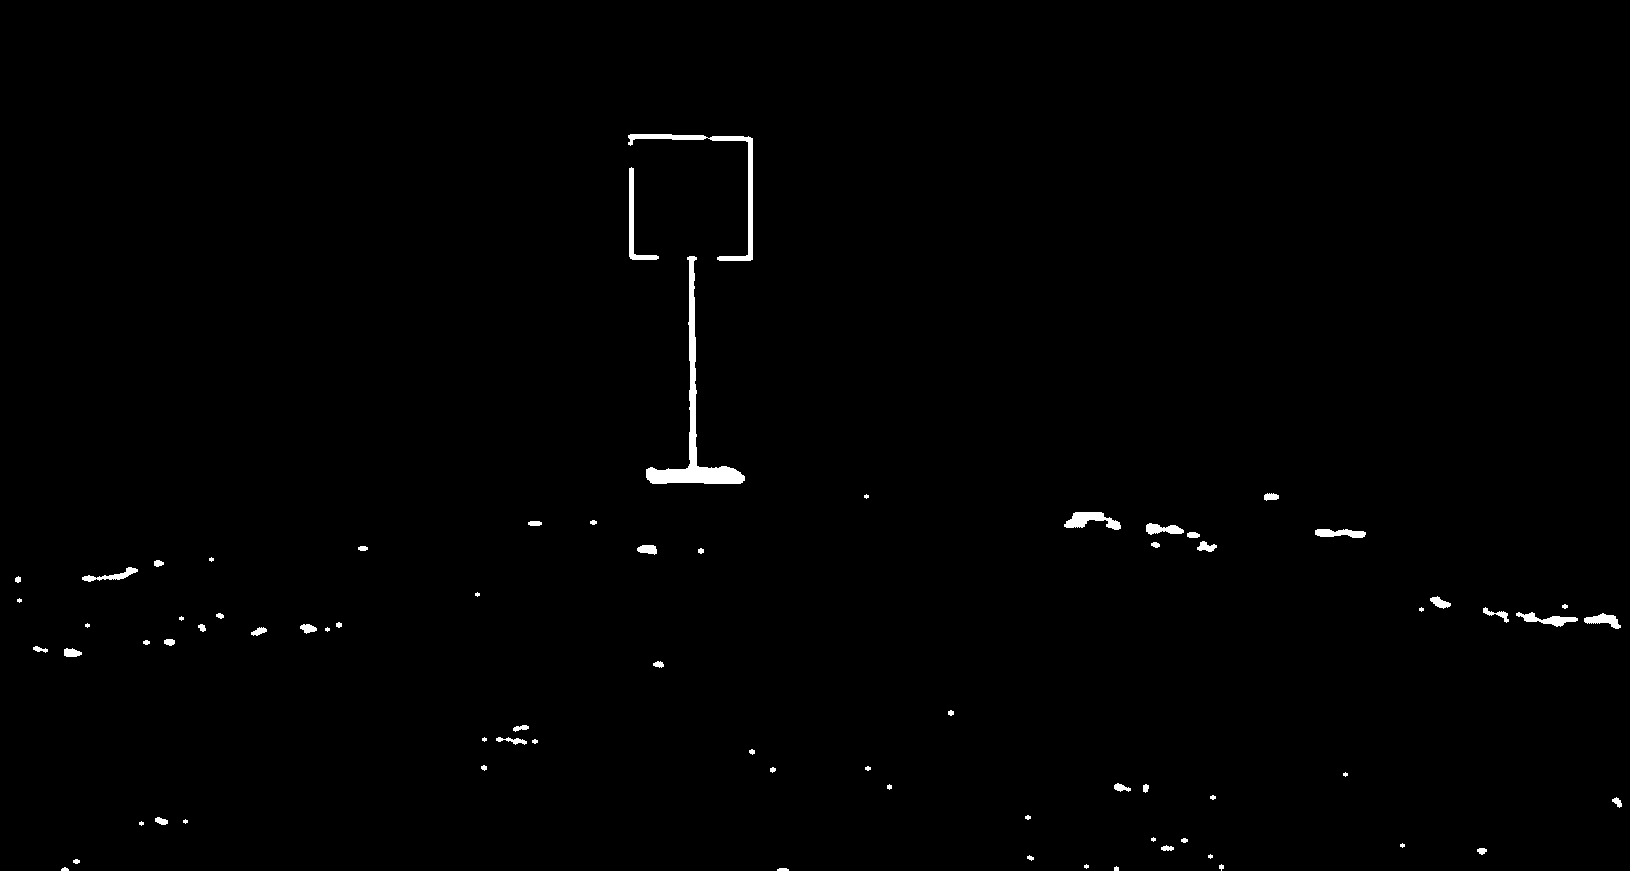
\includegraphics[width=0.48\textwidth]{Gate3_TH2.png}}}\hfill
    \subfloat[]{\label{fig:cv_gate4th2}{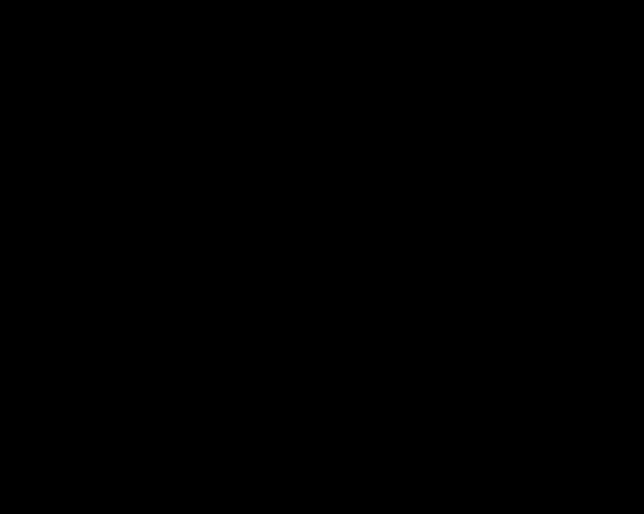
\includegraphics[width=0.48\textwidth]{Gate4_TH2.png}}}\hfill

    \caption{Sintonización del rango de color}
    \label{fig:cv_gatesth2}
\end{figure}

Recapitulando un poco lo ya comentado, el reajuste en la escala de color permitió obtener una mejora bastante significativa para la reducción de falsos positivos en la detección de las compuertas; sin embargo, contrario o lo que se esperaba, el desempeño que se obtuvo en la última imagen resulto ser inferior al de la primera prueba. Entonces, se buscó realizar una segunda sintonización con el objetivo de mejorar el desempeño en esta última imagen, por lo que ya no se realizaron más pruebas con las tres primeras imágenes, y el reajuste se realizó únicamente experimentando con esta última imagen. Sin embargo, pese a los esfuerzos realizados, no se logró encontrar un rango de valores que mejoraran la detección, simplemente el algoritmo no fue capaz de detectar la compuerta.

Lo anterior se atribuye a que, debido a la distancia con la que fue tomada la imagen, la proporción de superficie de las compuertas en la imagen es bastante reducida, por lo que el algoritmo no es capaz de aislar de manera satisfactoria el color que se busca. La figura \ref{fig:cv_gatesth3} presenta los resultados obtenidos con este último intento de resintonización. En la figura \ref{fig:cv_gate4th3} es posible observar el desempeño de la detección en la imagen objetivo, se puede apreciar que solamente fue posible mejorar el aislamiento de la fachada del edificio, dando como resultado el siguiente rango de parámetros:\[H:0-25;\text{ } S:45-217;\text{ } V:0-44\]

Entonces, se utilizó esta última escala de color para ejecutar la detección en el resto de fotografías, y lo que se obtuvo fue algo similar a lo observado en la figura \ref{fig:cv_gate1th3}. Esta figura corresponde solamente a la detección efectuada sobre la toma en primer plano de la compuerta, sin embargo, el resultado obtenido en las otras imágenes fue el mismo, un recuadro completamente negro.

Finalmente, está claro que este último rango de parámetros no es para nada eficiente y no cumple con el objetivo de la detección de compuertas, por lo que al final se descartó y se utilizó la escala obtenida a partir del primer ajuste para su implementación en ROS.

\begin{figure}[ht]
    \centering
    \subfloat[]{\label{fig:cv_gate1th3}{\includegraphics[width=0.48\textwidth]{Gate1_TH3.png}}}\hfill
    \subfloat[]{\label{fig:cv_gate4th3}{\includegraphics[width=0.48\textwidth]{Gate4_TH3.png}}}

    \caption{Intento de sintonización utilizando la cuarta imagen de referencia como base}
    \label{fig:cv_gatesth3}
\end{figure}

\section{Algoritmo de visón artificial}

En la sub-sección anterior se describió el proceso implementado para adecuar el algoritmo de detección con base en los requerimientos mencionados. Ahora, esta última sub-sección tiene como objetivo definir la lógica secuencial utilizada, así como las funciones que componen el algoritmo implementado.

La estructura de la lógica implementada puede observarse en el algoritmo \ref{alg:vision}
\begin{algorithm}
\caption{Metodología para la detección de compuertas}\label{alg:vision}
\begin{algorithmic}
\State \textbf{1. Adquirir} imagen
\State \textbf{2. Convertir }espacio de color: $\text{RGB} \to \text{BGR}$
\State \textbf{3. Convertir }espacio de color: $\text{BGR} \to \text{HSV}$
\State \textbf{4. Aplicar }el método del valor umbral sobre la imagen
\State \textbf{5. Aplicar }una operación de apertura sobre la imagen umbralizada
\State \textbf{6. Aplicar }una operación de cerradura sobre la imagen umbralizada
\State \textbf{6. Mostrar } la imagen original y la imagen procesada
\end{algorithmic}
\end{algorithm}

Como se puede observar, es un algoritmo bastante sencillo. Ahora bien, como se mencionó en el marco teórico, OpenCV ofrece una gran variedad de funciones y herramientas para la ejecución de algoritmos de visión artificial, por lo que el programa resultante es bastante compacto en cuanto a líneas de código, pues se utilizaron funciones nativas de la librería. El código desarrollado para esta etapa puede ser consultado en el repositorio oficial del presente trabajo \citet{Axolotl}, dentro del directorio de recursos.

A continuación se describen las funciones utilizadas para la implementación del algoritmo.

\textbf{imread}: recibe como argumentos el directorio de la imagen que se desea procesar y, de forma opcional, una bandera que indica algunos perfiles de color con los que puede ser leída la imagen. En este caso, solo se indicó el directorio para cargar cada imagen de forma individual en cada prueba. Cabe mencionar que OpenCV almacena las imágenes en una serie de arreglos multidimensionales, que dependiendo del perfil y el espacio de color, pueden ser manipulados a nivel de píxeles o capas.

\textbf{cvtColor}: es el método utilizado para realizar la conversión entre modelos de color; OpenCV es capaz de manejar distintos espacios de color, en el caso de este trabajo, primero se realizó la conversión del espacio RGB a BGR y después del BGR al HSV.

\textbf{inRange}: ejecuta el método del valor umbral. Recibe como parámetros la imagen que se desea procesar, y el limite inferior y superior del arreglo de valores HSV; este método crea una mascara con base en el rango de color, la cual es utilizada para aplicar las operaciones morfológicas necesarias y realizar el aislamiento del objeto que se desea detectar.

\textbf{erode}: ejecuta la operación morfológica de erosión, recibe la variable donde se almacena la imagen procesada, la imagen a procesar y el núcleo para llevar acabo la operación.

\textbf{dilate}: de forma similar a la función anterior, ejecuta la operación de dilación y recibe los mismos parámetros que la función de erosión.

\textbf{imshow}: despliega una ventana con una imagen indicada por el usuario. Recibe como parámetros el nombre de la ventana y la variable que almacena la imagen que se desea visualizar.

Por último, es importante mencionar que la operación de apertura, en el contexto del procesamiento de imágenes, consiste en ejecutar una operación de erosión seguida de una operación de dilación; por otro lado, para realizar una operación de cerradura, primero se ejecuta la erosión y después la dilación. La apertura sirve para remover los objetos pequeños del fondo, mientras que la cerradura ayuda a rellenar los huecos creados a partir del método del valor umbral, en el objeto que se desea detectar.

Lo anterior concluye la sección dedicada a la descripción del algoritmo de visón artificial implementado.


\chapter{Misión de vuelo}   

En esta sección se describe el proceso de implementación de los comandos de vuelo y el algoritmo de seguimiento de trayectoria para el vuelo a través del circuito; cabe mencionar que se siguió un paradigma similar al de la sección anterior, primero se trabajó con scripts individuales de Python, y una vez que se validó su funcionamiento, se creó su respectivo nodo en ROS; los resultados correspondientes a este último punto, se tratan a detalle en el capítulo dedicado a ROS.

Dicho lo anterior, el algoritmo de seguimiento de trayectoria se trabajó en pequeñas etapas, en donde se probaba una funcionalidad distinta del piloto automático, de tal forma que cada etapa integra a la anterior, y así de forma sucesiva hasta que se obtuvo el script con el algoritmo de misión de vuelo. Los códigos fuente pertenecientes a cada etapa se encuentran en el respectivo repositorio de GitHub, perteneciente al presente trabajo. La tabla \ref{tab:pymavlink} muestra la relación que existe entre cada etapa y su script en el repositorio de GitHub.

\begin{table}[ht]
    \centering
    \begin{tabular}{lll}
        \hline
         No. & Etapa & Código fuente\\
        \hline
        \hline
        1 & Establecimiento de la conexión entre Pymavlink y ArduPilot & listen.py\\
        2 & Configuración del modo de vuelo del dron & mode.py\\
        3 & Armado de motores y despegue & takeoff.py\\
        4 & Seguimiento de trayectoria con waypoints & movement.py\\
        5 & Implementación de la misión de vuelo & mission.py\\
        \hline
        \hline
    \end{tabular}
    \caption{Relación entre etapa y su código fuente}
    \label{tab:pymavlink}
\end{table}

A continuación se muestran los resultados obtenidos en cada una de las etapas mencionadas. 

\section{Conexión entre Pymavlink y ArduPilot}

Inevitablemente, lo primero que se realizó fue comprobar la comunicación entre el script de Pymavlink y el SITL de ArduPilot. Por esta razón, el script perteneciente a esta etapa es bastante sencillo; sin embargo, representa la base de las subsecciones posteriores.

A grandes rasgos, lo más destacable es la inclusión de la librería Pymavlink y la creación de un objeto que sirve como intermediario entre el script y el piloto automático simulado. Dicho esto, para crear el objeto es necesario especificar la dirección que se utilizará para entablar la conexión; esta se especifica al momento de iniciar el SITL de ArduPilot en un terminal. Además, ArduPilot provee dos direcciones para realizar la conexión. En este caso, se escogió la \textit{14551} de forma arbitraria, sin ninguna razón en específico. La figura \ref{fig:Ardupilot_Py} muestra la información generada por ArduPilot durante el inicio de una instancia del SITL, a simple vista es mucha información; sin embargo, los datos de interés para esta subsección se encuentran en la línea en donde se indican las direcciones disponibles para recibir los datos manejados por el piloto automático, al observar la figura de forma detenida es posible percatarse que hay dos direcciones denotadas por la palabra \textit{out}, la 127.0.0.1:14550 y la 127.0.0.1:14551, en donde los últimos 5 dígitos indican la dirección que se tiene que especificar en el script de Pymavlink para entablar comunicación con ArduPilot. 

\begin{figure}[ht]
    \centering
    \includegraphics[width=0.7\textwidth]{Ardupilot_Py.pdf}
    \caption{Datos de conexión de ArduPilot}
    \label{fig:Ardupilot_Py}
\end{figure}

Una vez que se entabló la conexión entre ambas partes es posible tener acceso a toda clase de datos de vuelo, entre ellos la actitud del dron. Cabe mencionar que, en los mensajes que recibe Pymavlink por parte de ArduPilot es una trama de datos de gran longitud, y debido a que se creó un objeto de Python para entablar la conexión, es posible acceder a un dato en específico como se accede a un atributo en la instancia de una clase. En este caso, se decidió imprimir en consola el dato del ángulo de roll de dron con el fin de comprobar que la comunicación se dio de forma exitosa. 

Por último con respecto a esta subsección, la figura \ref{fig:pymav_listen} muestra el resultado de haber entablado una comunicación exitosa entre Pymavlink y el piloto automático, en la figura \ref{fig:pymav_atitude} se logra apreciar la trama completa con los datos referentes a la actitud del dron al momento de llevar a cabo la comunicación, mientras que la figura \ref{fig:pymav_roll} presenta esta trama de forma filtrada, de tal manera que solo se imprime el ángulo de roll del dron.
 

\begin{figure}[ht]
    \centering
    \subfloat[Trama de datos de la actitud del dron]{\label{fig:pymav_atitude}{\includegraphics[width=0.95\textwidth]{pymav_atitude.pdf}}}\\
    \subfloat[Datos del roll]{\label{fig:pymav_roll}{\includegraphics[width=0.4\textwidth]{pymav_roll.pdf}}}
    \caption{Datos obtenidos a partir de la conexión entre ArduPilot y Pymavlink} 
    \label{fig:pymav_listen}
\end{figure}


\section{Configuración de modo de vuelo}

De acuerdo con la documentación oficial de ArduPilot \cite{Ardu_modes}, el Arducopter cuenta con una gran variedad de modos de vuelo, no obstante, en este trabajo solo se utilizan únicamente dos modos, \textit{guided} y \textit{land}; el primero permite enviar comando de vuelo de forma directa al piloto automático a través de mensajes, mientras que el segundo ejecuta una rutina de aterrizaje para el dron. Este último modo de vuelo se aborda en la subsección marcada como extra.

Entonces, previo a la secuencia de despegue del dron, es necesario configurar el modo de vuelo en guided, pues al iniciar el SITL de ArduPilot, este inicializa con el modo de vuelo "stabilize", de tal forma que el piloto automático no es capaz de recibir comandos de vuelo ingresado directamente por el usuario. Esto representa un problema pues se busca que la trayectoria de vuelo del dron sea determinada a partir de un conjunto predefinido de waypoints.

Con base en lo anterior, el script perteneciente a esta subsección busca el identificador perteneciente al modo de vuelo indicado, dentro de una tabla de valores pre-configurados dentro de la librería, y utiliza el objeto de la subsección anterior para enviar el comando de selección de modo de vuelo al piloto automático. En dado caso de que el modo de vuelo especificado tenga un registro válido dentro de la tabla de la librería, se imprime un mensaje en donde se confirma que el modo de vuelo ha sido cambiado.

Por último, el método utilizado para establecer el modo de vuelo fue \textit{set\_mode\_send}, el cual recibe solamente 3 parámetros, el atributo del sistema del objeto de la conexión, el comando para establecer el modo de vuelo, y el código de identificación del modo de vuelo especificado. La figura \ref{fig:pymav_modes} muestra el resultado que se obtuvo al ejecutar el código desarrollado para esta subsección, en la figura \ref{fig:pymav_mode} se observa el mensaje de ejecución del script como tal, y por otro lado, la figura \ref{fig:Ardupilot_mode} presenta la aceptación del comando y el cambio de modo de vuelo reflejado en la terminal de ArduPilot.


\begin{figure}[ht]
    \centering
    \subfloat[Respuesta en Pymavlink]{\label{fig:pymav_mode}{\includegraphics[width=0.48\textwidth]{pymav_mode.pdf}}}\hfill
    \subfloat[Respuesta en ArduPilot]{\label{fig:Ardupilot_mode}{\includegraphics[width=0.48\textwidth]{Ardupilot_mode.pdf}}}
    \caption{Ejecución del script para la configuración del modo de vuelo}
    \label{fig:pymav_modes}
\end{figure}


\section{Secuencia de despegue}

Una vez que se logró entablar la comunicación con el piloto automático y se seleccionó en modo de vuelo adecuado, la secuencia de despegue resulto bastante sencilla de implementar, pues solo consta de dos pasos; enviar el comando para el armado de motores y enviar el comando de despegue especificando la altura deseada. Sin embargo, para que lo anterior se logre ejecutar de manera correcta, es necesario esperar a que los sistemas de la computadora de vuelo se inicialicen por completo, en especial aquellos sensores que sirven para la estimación de posición del dron, pues se requiere de estos para que el dron pueda despegar y elevarse a la altura solicitada por el usuario.

Esto último representó un problema al momento de crear el nodo de la misión de vuelo en ROS, pues si los filtros de estimación no se encuentran listos al momento de ejecutar el comando de despegue, la instrucción no se ejecuta y el dron es incapaz de iniciar su rutina de vuelo. La solución a este problema se aborda en la respectiva sección de ROS.

Dicho lo anterior, el script perteneciente a esta subsección no cuenta con la etapa de la selección del modo de vuelo, pues es necesario ejecutar el programa en el momento en el que los filtros del sistema han sido inicializados, y si se corre el script al mismo tiempo que  se inicia el SITL, el comando de despegue es rechazado. Entonces, para ejecutar el programa, el usuario tiene que cambiar el modo de vuelo de forma manual dentro de la terminal de ArduPilot, de esta forma se asegura que el sistema está listo para recibir la instrucción de despegue.

Además, en este caso el script envía los comandos al piloto automático mediante la instrucción command\_long\_send, la cual recibe 11 parámetros; en donde los primeros 2 corresponden al sistema y al componente de MAVLink, los cuales son atributos pertenecientes al objeto creado al momento de establecer la comunicación con el piloto automático. Por otro lado, el siguiente parámetro corresponde al comando de vuelo que se desea enviar y los siguientes 8 sus respectivos atributos. Recordando que un comando de MAVLink puede recibir hasta 7 atributos, existen muchos comando en donde no se ocupan por completo esta cantidad de atributos, en estos casos, es necesario revisar la documentación perteneciente al comando en cuestión y verificar la cantidad especifica de atributos requeridos, el resto de parámetros no utilizados se debe de dejar en 0.

Entonces, en el caso de esta etapa, los comandos de vuelo utilizados fueron \textit{MAV\_ CMD\_COMPONENT\_ARM\_DISARM} para el armado de los motores y \textit{MAV\_CMD\_NAV\_ TAKEOFF} para la orden de despegue. La figura \ref{fig:pymav_takeoff} muestra el comportamiento observado en la simulación tras la ejecución del script con la secuencia de despegue, la figura \ref{fig:pymav_takeoff1} presenta el estado inicial de la simulación, antes de que se enviara el comando de vuelo, por otro lado, la figura \ref{fig:pymav_takeoff2} muestra el dron en vuelo, tras haber alcanzado la altura indicada en el comando de vuelo. Entonces, a simple vista se logra apreciar que el comando se ejecutó de manera correcta y el dron despega sin ningún tipo de problema.  

\begin{figure}[ht]
    \centering
    \subfloat[]{\label{fig:pymav_takeoff1}{\includegraphics[width=0.48\textwidth]{pymav_takeoff1.jpg}}}\hfill
    \subfloat[]{\label{fig:pymav_takeoff2}{\includegraphics[width=0.48\textwidth]{pymav_takeoff2.jpg}}}
    \caption{Comportamiento de la simulación ante el comando de despegue}
    \label{fig:pymav_takeoff}
\end{figure}


Si bien la figura \ref{fig:pymav_takeoff} muestra de manera acertada la correcta ejecución de la secuencia de despegue, a simple vista resulta difícil decir con exactitud sin el dron alcanzó, o no, la altura desea. Debido a lo anterior, se recopilaron los datos correspondientes a la posición y velocidad del dron durante su ascenso, a partir de uno de los mensajes de MavLink que permite obtener acceso a esta información manejada por el piloto automático. En consecuencia, la figura \ref{fig:pymav_takeoffz} es una gráfica que muestra la altura del dron durante su despegue, de tal forma que es posible apreciar que, en efecto, el dron logra alcanzar la altitud deseada durante su despegue con un ligero sobre paso, aproximadamente a los 13 segundos después de comenzar a ejecutar el comando de vuelo. Por otro lado, cabe mencionar que, debido al marco de referencia con el que se está trabajando, un desplazamiento hacia arriba en el eje \textit{z} es considerado negativo, mientras que un desplazamiento hacia abajo en ese eje se considera positivo; sin embargo, para fines de una interpretación de datos más intuitiva, se invirtió el signo de la lectura de datos en el eje \textit{z}. 

\begin{figure}[h]
    \centering
    \includegraphics[width=0.7\textwidth]{pymav_takeoffz.pdf}
    \caption{Respuesta en la altura para el comando de despegue.}
    \label{fig:pymav_takeoffz}
\end{figure}

Adicionalmente, la figura \ref{fig:pymav_takeoffvz} corresponde a una gráfica que describe el comportamiento de la velocidad de ascenso del dron, y de manera congruente con la gráfica mencionada anteriormente, se puede apreciar un descenso en la velocidad de ascenso en el intervalo de tiempo de 10 s y 15 s, lapso en el que el dron logra llegar a la referencia y por lo tanto ya no es necesario ascender más;  además, se observa una velocidad máxima de ascenso de 2.21 $\frac{m}{s}$.

\begin{figure}[ht]
    \centering
    \includegraphics[width=0.7\textwidth]{pymav_takeoffvz.pdf}
    \caption{Gráfica de velocidad de despegue.}
    \label{fig:pymav_takeoffvz}
\end{figure}

\section{Seguimiento de trayectoria}

Hecho todo lo anterior, la última prueba que se tuvo que realizar, en cuanto a una funcionalidad en específico de Pymavlink, fue la del seguimiento de trayectoria por medio de comandos de vuelo directos, en forma de waypoints. Sin embargo, debido al problema mencionado en la etapa anterior, el script perteneciente a esta subsección no ejecuta las etapas anteriores, sino que para poder ejecutar el programa, el usuario tiene que esperar a que la terminal de Ardupilot permita el cambio de modo de vuelo de forma manual, y después ejecutar los respectivos comandos de vuelo para realizar la secuencia de despegue del dron.

Ahora bien, la prueba realizada para esta etapa fue sencilla, se enviaron dos waypoint utilizando el marco de referencia local, en donde el origen, o la coordenada (0,0,0), corresponde al punto inicial del mundo creado, denotado de forma visual por 3 barras ortogonales de color azul para el eje \textit{z}, azul para el eje \textit{x} y verde para el eje \textit{y}. Además, como se mencionó, la trayectoria de vuelo está compuesta por dos waypoints, los cuales fueron definidos de tal manera que se buscó que el dron cruzara por las dos primeras compuertas del circuito de vuelo, dichos waypoint son [35,0,3] y [35, 17, 2]; Dicho esto, la secuencia pensada para la ejecución de esta prueba fue, primero hacer ascender el dron a una altura de 10 m y después indicarle su trayectoria de vuelo a partir de los waypoints especificados. 

Asimismo, se buscó comprobar si el piloto automático espera a que el dron llegue al primer waypoint para dirigirse hacía el segundo, sin embargo, esto no sucede y el piloto automático ejecuta el segundo waypoint definido, pues no hay ningún tiempo de espera o bandera que le indique al piloto que debe de esperar a que se termine la ejecución del primer waypoint. Entonces, para evitar que el piloto automático ignorara el primer waypoint, se utilizó un mensaje de MAVLink definido como \textit{NAV\_CONTROLLER\_OUTPUT} el cual publica información relacionada sobre el comando de vuelo enviado al piloto automático, entre la cual se encuentra la distancia faltante para que el dron llegue al waypoint especificado al momento de lectura del mensaje. Entonces, la instrucción para el seguimiento del segundo waypoint es enviada al piloto automático hasta que el mensaje especifica que la distancia restante para llegar al primer waypoint es igual a cero.

Continuando con los resultados de la prueba, en este caso el script solo ejecuta las instrucciones para guiar el vuelo del dron, por lo que es necesario que el usuario realice todo el pre-proceso necesario para el despegue del dron. En el caso de la prueba realizada la altitud de despegue indicada fue de 10 m, por lo que para el seguimiento del waypoint, el dron tuvo que descender a 3 m de altura al mismo tiempo que avanzó 10 m en el eje x, y después otros 20 m. Cabe mencionar que para el piloto automático, una altura negativa indica un punto sobre la referencia inicial, y análogamente, una altura positiva corresponde a un punto por debajo de la referencia inicial. 

Además, los waypoints son enviados utilizando el comando de vuelo \textit{MAVLink\_set\_ position\_target\_local\_ned\_message}, el cual requiere 16 parámetros para realizar el seguimiento de un waypoint. La tabla \ref{tab:waypoint} enlista los parámetros y muestra una breve descripcción de los mismos; Por otro lado, el parámetro type\_mask  es algo complejo de explicar, por lo que, por motivos de practicidad y legibilidad, se describe a más detalle fuera de la tabla.

Retomando lo anterior, el parámetro type\_mask indica la cantidad de parámetros que el comando de vuelo tiene que tomar en cuenta de acuerdo a lo que el usuario desee indicar, dígase posición, velocidad, aceleración o las tres magnitudes anteriores. Dicho esto, mencionando un ejemplo, si se desea enviar un comando de velocidad, es necesario especificar la velocidad de referencia para los 3 ejes cartesianos y el resto de parámetros serán ignorados independiente del valor indicado en el comando.

Adicionalmente, la tabla \ref{tab:waypoint_mask} muestra los distintos valores que se le pueden asignar al parámetro de máscara. En el caso de este trabajó se utilizó el primer tipo de máscara, debido a que solo se buscó que el dron siguiera una trayectoria, con la máxima velocidad que el vehículo pudiera proporcionar.

\begin{table}[ht]
    \centering
    \begin{tabular}{ll}
        \hline
        Parámetro & Descripción\\
        \hline
        \hline
        time\_boot\_ms & Tiempo de arranque del sistema en ms\\
        target\_system & Identificador del sistema\\
        target\_component & Identificador del componente o controlador de vuelo\\
        coordinate\_frame & Marco de referencia\\
        type\_mask & Indica los campos que se deben de ignorar\\
        x & Posición en el eje \textit{x} en m\\
        y & Posición en el eje \textit{y} en m\\
        z & Posición en el eje \textit{z} en m\\
        vx & Velocidad en el eje \textit{x} en m/s\\
        vy & Velocidad en el eje \textit{y} en m/s\\
        vz & Velocidad en el eje \textit{z} en m/s\\
        afx & Aceleración en el eje \textit{x} en m/$s^2$\\
        afy & Aceleración en el eje \textit{y} en m/$s^2$\\
        afz & Aceleración en el eje \textit{z} en m/$s^2$\\
        yaw & Ángulo de guiñada en radianes\\
        yaw rate & Aceleración de la guiñada en rad/s\\
        \hline
        \hline
    \end{tabular}
    \caption{Parámetros de la instrucción para seguimiento de waypoints}
    \label{tab:waypoint}
\end{table}

\begin{table}[ht]
    \centering
    \begin{tabular}{llll}
        \hline
        Tipo & Binario & Hexadecimal & Decimal\\
        \hline
        \hline
        Posición & 0b110111111000 & 0x0DF8  & 3576 \\
        Velocidad & 0b110111000111 & 0x0DC7  & 3527\\
        Aceleración & 0b110000111111 & 0x0C3F & 3135 \\
        Pos + Vel & 0b110111000000 & 0x0DC0 & 3520\\  
        Pos + Vel + Acel & 0b110000000000 & 0x0C00 & 3072\\
        Guiñada & 0b100111111111 &  0x09FF & 2559\\
        Velocidad de  guiñada& 0b010111111111  & 0x05FF & 1535\\
        \hline
        \hline
    \end{tabular}
    \caption{Tipos de máscara para el comando de seguimiento de trayectoria}
    \label{tab:waypoint_mask}
\end{table}

Ahora bien, retomando el contexto de los resultados obtenidos al momento de ejecutar el script desarrollado para esta subsección, 
la figura \ref{fig:pymav_movement} presenta el comportamiento observado en la simulación tras la ejecución de la secuencia de comando especificada para esta subsección. Entonces, en la figura \ref{fig:pymav_movement1} se observa el estado inicial del dron, previo a la ejecución del protocolo; la figura \ref{fig:pymav_movement2} muestra el dron después de haber ascendido a la altura de 10 m (la cual fue comandada de forma manual a través de la terminal de ArduPilot); Por otro lado, pese a que se mencionó que los waypoints se definieron con el fin de que el dron fuera capaz de cruzar las primeras dos compuertas del circuito de vuelo, en la figura \ref{fig:pymav_movement3} se aprecia que el dron sobrevuela la primera compuerta del circuito y no para a través de ella, esto se debe a la altura de ascenso que se definió durante la prueba, sin embargo, cabe mencionar que si al dron se le comanda un despegue de 3 m (altura a la que se encuentra el centro de las compuertas grandes), este es capaz de cruzar por el centro de las dos primeras compuertas utilizando los dos waypoints definidos; asimismo, la figura \ref{fig:pymav_movement4} muestra una captura del dron después de que este llegó a su punto final tras seguir el segundo waypoint, se aprecia que en este caso el dron si fue capaz de cruzar a través de la segunda compuerta.

\begin{figure}[ht]
    \centering
    \subfloat[]{\label{fig:pymav_movement1}{\includegraphics[width=0.48\textwidth]{pymav_movement1.jpg}}}\hfill
    \subfloat[]{\label{fig:pymav_movement2}{\includegraphics[width=0.48\textwidth]{pymav_movement2.jpg}}}\\
    \subfloat[]{\label{fig:pymav_movement3}{\includegraphics[width=0.48\textwidth]{pymav_movement3.jpg}}}\hfill
    \subfloat[]{\label{fig:pymav_movement4}{\includegraphics[width=0.48\textwidth]{pymav_movement4.jpg}}}\hfill

    \caption{Etapas de la prueba de seguimiento de trayectoria}
    \label{fig:pymav_movement}
\end{figure}

De manera similar a la subsección anterior, la figura \ref{fig:pymav_movement} permite observar de manera rápida y práctica si el comportamiento del dron fue el adecuado; sin embargo, el análisis del desempeño del dron se logra a partir de los datos de vuelo recopilados. La figura \ref{fig:pymav_movementxy} muestra una gráfica en donde se describe la trayectoria de vuelo seguida por el dron, en ella se especifica la ubicación de las compuertas con base en el recorrido descrito. Cabe mencionar que, contrario a lo que se considera intuitivo, el desplazamiento a lo largo del eje \textit{x} se observa en el eje vertical, mientras que el desplazamiento en el eje \textit{y} corresponde al eje horizontal, esto es debido a que de esta forma la gráfica es congruente con la perspectiva de la cámara dentro de la simulación. En consecuencia, se puede decir que, a partir de la figura \ref{fig:pymav_movementxy}, el dron siguió los waypoints de manera satisfactoria, logrando completar una ruta de vuelo simple. 

\begin{figure}[ht]
    \centering
    \includegraphics[width=0.8\textwidth]{pymav_movementxy.pdf}
    \caption{Recorrido realizado por el dron}
    \label{fig:pymav_movementxy}
\end{figure}

De forma subsecuente, la figura \ref{fig:pymav_movementd} presenta el comportamiento del desplazamiento lineal del dron a lo largo de los tres ejes espaciales. La figura \ref{fig:pymav_movementx} corresponde al desplazamiento en el eje \textit{x}, en ella se observa como es que el dron llega a la referencia de 35 m sin ningún sobre paso, en un tiempo de aproximadamente 10 s; una vez que el dron completa la trayectoria definida por el primer waypoint, este gira a la izquierda para dirigirse al segundo waypoint, de tal forma que ya no se observa un desplazamiento en el eje \textit{x}, sino, en el eje \textit{y}, en consecuencia, el desplazamiento observado en la gráfica de la figura \ref{fig:pymav_movementy} ocurre hasta el segundo 10, que es cuando se da la transición entre waypoints. Por último, en la gráfica de la figura \ref{fig:pymav_movementz} se logra apreciar el cambio de altura durante el vuelo del dron, resulta evidente la forma en la que el dron desciende de los 10 m indicados en su despegue a una primera referencia de 3 m, y posteriormente el lapso de transición entre waypoints desciende 1 m más, pues la segunda compuerta es más pequeña y está más cerca del suelo; en ambos casos logra el dron logra llegar a la altura indicada.

\begin{figure}[ht]
    \centering
    \subfloat[Eje X]{\label{fig:pymav_movementx}{\includegraphics[width=0.48\textwidth]{pymav_movementx.pdf}}}\hfill
    \subfloat[Eje Y]{\label{fig:pymav_movementy}{\includegraphics[width=0.48\textwidth]{pymav_movementy.pdf}}}\\
    \subfloat[Eje Z]{\label{fig:pymav_movementz}{\includegraphics[width=0.48\textwidth]{pymav_movementz.pdf}}}\hfill

    \caption{Gráficas de desplazamiento para los tres ejes}
    \label{fig:pymav_movementd}
\end{figure}

Asimismo, el conjunto de gráficas en la figura \ref{fig:pymav_movementv}, esta esta relacionada con las velocidades lineales asociadas a cada uno de los 3 ejes de desplazamiento del dron. Dicho lo anterior, en la figura \ref{fig:pymav_movementvx}, se observa como en el eje \textit{x} se alcanza la velocidad máxima de 8.34 $\frac{m}{s}$, en el segundo 3.75, antes del tiempo de transición de waypoints, de tal manera que para el segundo 10, la velocidad a lo largo de este eje ha decrecido de forma significativa y de forma intuitiva, se aprecia en la figura \ref{fig:pymav_movementvy} que como es que la velocidad a lo largo del eje \textit{y} comienza su ascenso a partir del tiempo de transición de waypoints, llegando un máximo de 5.59 $\frac{m}{s}$ en el segundo 11.25 del vuelo del dron. 

Por otra parte, la figura \ref{fig:pymav_movementvz} muestra el comportamiento de la velocidad a lo largo del eje \textit{z}; es importante no perder de vista que, como se mencionó en la subsección de la etapa de despegue, los signos de las velocidades fueron invertidos para que el análisis de resultados correspondiera de forma visual con el comportamiento observado durante la ejecución de la simulación. Dicho esto, en la figura \ref{fig:pymav_movementvz} se destaca una pendiente negativa en los primeros 2 segundos de la simulación, esto se debe a que el dron inició a una altura de 10 m y tuvo que descender a 3 m, por lo que el sentido del vector de velocidad fue hacia abajo, llegando a una velocidad de -1.56 $\frac{m}{s}$ en el segundo 2, después de este lapso, el dron tuvo que disminuir su velocidad pues se fue aproximando cada vez más a la altura deseada de 3 m, lo cual ocurrió poco después del segundo 5, con base en la figura \ref{fig:pymav_movementz}; en la gráfica se puede observar un pequeño sobrepaso con una velocidad positiva de 0.0634 $\frac{m}{s}$. Luego, un poco antes del segundo 10, ocurre la transición al siguiente waypoint, por lo que el dron tuvo que descender a los 2 m de altura, una vez más, presentando una velocidad negativa para después detenerse de forma gradual hasta llegar a la altura de referencia. Por último, se observa que el dron finaliza con su recorrido aproximadamente en el segundo 15, pues la velocidad se mantiene en cero después de ese punto.

\begin{figure}[ht]
    \centering
    \subfloat[Eje X]{\label{fig:pymav_movementvx}{\includegraphics[width=0.48\textwidth]{pymav_movementvx.pdf}}}\hfill
    \subfloat[Eje Y]{\label{fig:pymav_movementvy}{\includegraphics[width=0.48\textwidth]{pymav_movementvy.pdf}}}\\
    \subfloat[Eje Z]{\label{fig:pymav_movementvz}{\includegraphics[width=0.48\textwidth]{pymav_movementvz.pdf}}}\hfill

    \caption{Comportamiento de la velocidad lineal de vuelo en los tres ejes}
    \label{fig:pymav_movementv}
\end{figure}

Por último con respecto a esta prueba, la figura \ref{fig:pymav_pathfollowing} presenta una proyección en 3D del la trayectoria de vuelo ejecutada por el dron. Esta gráfica presenta de manera más visual la ruta observada durante la ejecución de la simulación y es posible observar los 3 instantes más significativos de esta prueba. Primero, el dron inicia con una altura de 10 m; después se le comanda el primer waypoint [35,0,3], lo que corresponde al descenso pronunciado observado en la gráfica; cuando el dron llega a su primera referencia, se le comanda el segundo waypoint [35,17,2], donde se observa otro descenso, menos pronunciado y un movimiento a lo largo del eje \textit{y}.

\begin{figure}[ht]
    \centering
    \includegraphics[width=0.45\textwidth]{pymav_pathfollowing.pdf}
    \caption{Gráfica en 3D de la trayectoria seguida por el dron.}
    \label{fig:pymav_pathfollowing}
\end{figure}

\section{Misión de vuelo}

Con la etapa anterior se culminaron las pruebas por módulos; en esta subsección se describe el proceso realizado para integrar todas las etapas descritas hasta el momento.

Debido a que se trabajó con un paradigma de módulos, en donde cada etapa descrita corresponde a un módulo y/o funcionalidad especifica, la unificación de todo lo anteriormente descrito resultó ser un proceso bastante lineal y práctico, en la mayor parte de las etapas se utilizó el mismo código desarrollado para su respectivo script; Por otro lado, en esta etapa se buscó implementar de forma completa la misión de vuelo para el dron, de tal manera que fuera capaz de cruzar a través de las 4 compuertas que componen el circuito de vuelo, por lo tanto, la misión de vuelo cuenta con 4 waypoints, los cuales se muestran en la tabla \ref{tab:waypoints_mission}.

\begin{table}[ht]
    \centering
    \begin{tabular}{ccc}
        \hline
        x & y & z\\
        \hline
        \hline
        35 & 0 & 3\\
        35 & 17 & 2\\
        0 & 17 & 3\\
        0 & 0 & 3\\
        \hline
        \hline
    \end{tabular}
    \caption{Waypoints utilizados en la misión de vuelo}
    \label{tab:waypoints_mission}
\end{table}


Dicho lo anterior, a manera de recapitulación, se describen los módulos en el orden en el que fueron implementados en el script de esta subsección:

\begin{enumerate}
    \item Establecimiento de comunicación entre Pymavlink y ArduPilot
    \item Cambio de modo de vuelo de stabilize a guided
    \item Armado de motores
    \item Envío de orden de despegue
    \item Envío de comandos de vuelo para seguimiento de waypoints
\end{enumerate}

Adicionalmente, el script de misión de vuelo busca eliminar la necesidad de que el usuario tenga que introducir comando de vuelo de forma manual en la terminal de ArduPilot; es decir, solo es necesario ejecutar el script y el dron será capaz de ejecutar todas las etapas descritas.

Ahora bien, la figura \ref{fig:pymav_mission} muestra el comportamiento observado en simulación tras haber ejecutado el script de la misión de vuelo, de tal manera que en la figura \ref{fig:pymav_mission1} se observa como el dron es capaz de cruzar por el centro de la primera compuerta; la figura \ref{fig:pymav_mission2} presenta el cruce por la segunda compuerta; la figura \ref{fig:pymav_mission3} corresponde al waypoint para la tercera compuerta y por último en la figura \ref{fig:pymav_mission4} se observa el estado final del dron tras haber atravesado la cuarta compuerta. Entonces, a partir de la figura \ref{fig:pymav_mission} es posible apreciar, a simple vista, como el dron logró completar el circuito de vuelo de forma exitosa.  

\begin{figure}[ht]
    \centering
    \subfloat[]{\label{fig:pymav_mission1}{\includegraphics[width=0.48\textwidth]{pymav_mission1.jpg}}}\hfill
    \subfloat[]{\label{fig:pymav_mission2}{\includegraphics[width=0.48\textwidth]{pymav_mission2.jpg}}}\\
    \subfloat[]{\label{fig:pymav_mission3}{\includegraphics[width=0.48\textwidth]{pymav_mission3.jpg}}}\hfill
    \subfloat[]{\label{fig:pymav_mission4}{\includegraphics[width=0.48\textwidth]{pymav_mission4.jpg}}}\hfill

    \caption{Seguimiento de misión de vuelo completa}
    \label{fig:pymav_mission}
\end{figure}

De forma similar a la subsección correspondiente al seguimiento de trayectoria, la figura \ref{fig:pymav_missionxy} presenta la ruta de vuelo realizada por el dron. Se vuelve a destacar que, contraintuitivamente, el desplazamiento entre los ejes se encuentra acomodado de tal manera que correspondan a la perspectiva con la que se observó el vuelo del dron; es decir, como si se estuviera viendo el desplazamiento del dron como se observa en la figura \ref{fig:pymav_mission}. Además, la figura \ref{fig:pymav_missionxy} cuenta con la ubicación de las cuatro compuertas del circuito de vuelo, así como el sentido de vuelo que siguió el dron durante su recorrido. A partir de esto, se logra apreciar que los waypoints fueron definidos de tal manera que el dron describiera una trayectoria rectangular uniforme, por lo tanto, la trayectoria recorrida por cada waypoint corresponde a cada una de las artistas del rectángulo y la transición entre cada uno está representado por los vértices de este. 

Por otro lado, cabe mencionar que MAVLink acepta misiones de vuelo de forma nativa, en donde solo es necesario cargar un archivo de texto en donde se defina la serie de waypoints que se desean seguir, por medio de coordenadas según el marco de referencia; sin embargo, al tiempo de desarrollo de este trabajo, no se encontró ningún comando de vuelo aceptado por PymavLink que permitiera cargar de forma sencilla una misión de vuelo, por lo que, la trayectoria de vuelo implementada se realizó a partir de una función desarrollada desde cero, en donde los waypoints son enviados de forma explícita y de uno en uno, debido a esto fue necesario implementar la solución mencionada en la subsección anterior, en donde por medio de un mensaje es posible conocer la distancia restante para que el dron complete la trayectoria de cada waypoint.

\begin{figure}[ht]
    \centering
    \includegraphics[width=0.75\textwidth]{pymav_missionxy.pdf}
    \caption{Recorrido realizado por el dron}
    \label{fig:pymav_missionxy}
\end{figure}

Siguiendo con los resultados obtenidos en esta subsección, la figura \ref{fig:pymav_missiond} muestra el desplazamiento lineal capturado durante el vuelo del dron. Es posible observar un comportamiento bastante peculiar en todos los ejes, por un lado en la figura \ref{fig:pymav_missionx} se puede apreciar como para el primer waypoint el desplazamiento en el eje \textit{x} incrementa de forma gradual hasta llegar a 35 m, en aproximadamente 10 segundos, después, ocurre la transición para el segundo waypoint, sin embargo la posición en el eje \textit{x} se mantiene intacta, por eso el dron permanece en 35, hasta el segundo 16, en donde ocurre la transición al tercer waypoint y es necesario disminuir el desplazamiento hasta llegar a 0 m en el eje \textit{x}, en donde el dron se mantiene hasta finalizar su recorrido. Por otro lado, en la figura \ref{fig:pymav_missiony} se aprecia un comportamiento en el eje \textit{y} de cierta forma complementario al del eje \textit{x}, en los primeros 10 segundos del recorrido, el dron no presenta ningún desplazamiento en \textit{y} por lo que su posición con respecto a este eje se mantiene en 0, posteriormente, ocurre la transición al segundo waypoint y es cuando ocurre el primer desplazamiento en \textit{y}, de tal forma que el dron avanza 17 m, después, en el segundo 25, se da la transición al tercer waypoint y la posición en \textit{y} comienza a decrementar, de tal forma que para el segundo 30 el dron ya se encuentra en el origen del circuito de vuelo. De manera similar, a partir de la figura \ref{fig:pymav_missionz} es posible intuir el comportamiento de la altura del dron durante su vuelo, el cual resulta ser más sencillo que los dos anteriores pues en este caso, la altitud solamente osciló entre dos valores 3 y 2 m, donde a los 10 segundos de vuelo ocurre un descenso a los 2 m de altura, pues ocurre la transición al segundo waypoint y la compuerta correspondiente  a este waypoinzt es de menor tamaño, por lo que es necesario que el dron descienda y luego vuelva a ascender a los 3 m cuando ocurre la siguiente transición de waypoints.

\begin{figure}[ht]
    \centering
    \subfloat[Eje X]{\label{fig:pymav_missionx}{\includegraphics[width=0.48\textwidth]{pymav_missionx.pdf}}}\hfill
    \subfloat[Eje Y]{\label{fig:pymav_missiony}{\includegraphics[width=0.48\textwidth]{pymav_missiony.pdf}}}\\
    \subfloat[Eje Z]{\label{fig:pymav_missionz}{\includegraphics[width=0.48\textwidth]{pymav_missionz.pdf}}}\hfill

    \caption{Gráficas de desplazamiento para los tres ejes}
    \label{fig:pymav_missiond}
\end{figure}

 Así mismo, la figura \ref{fig:pymav_missionv} presenta el comportamiento de la velocidad lineal en los tres ejes de desplazamiento. La gráfica de la figura \ref{fig:pymav_missionvx} presenta el comportamiento en el eje \textit{x}, mientras que la figura \ref{fig:pymav_missionvy} hace lo respectivo con el eje \textit{y}; como se observa, ambas gráficas presentan comportamientos bastantes similares. El primer waypoint 35,0,3 involucra un desplazamiento positivo en el eje \textit{x}, sin desplazarse en el eje \textit{y}, por lo que en los primeros 10 segundos de la simulación se observa el máximo en $v_x$ de 8.42 $\frac{m}{s}$, mientras que $v_y$ permanence en 0; el decremento de $v_x$ se debe a que el dron comienza a detenerse conforme se acerca a la referencia de posición, y poco antes del segundo 10 se observa un incremento en $v_y$, debido a la transición al segundo waypoint 35,17,2, donde $v_y$ alcanza su máximo de 5.53 $\frac{m}{s}$ en el segundo 11.25 para después disminuir su velocidad.
 
 Luego, se observa una pendiente negativa en $v_x$ pues el tercer waypoint [0,17,3] implica un retroceso en el desplazamiento en \textit{x}, de tal forma que después del segundo 18.5 también se observa una reducción en la magnitud de $v_x$ hasta llegar a cero. Este comportamiento también se observa para el cuarto waypoint [0,0,0] en donde $v_y$ presenta la pendiente negativa y posteriormente un detenimiento completo.

 Por último, en la figura \ref{fig:pymav_missionvz} es posible observar el comportamiento de $v_z$. Se aprecia que al inicio de la gráfica se presenta el máximo de velocidad (0.67 $\frac{m}{s}$), esto se debe a que la adquisición de datos comenzó justo después de que la etapa de despegue hubiera concluido, por lo que el dron ya contaba con cierta velocidad, después de eso, se observan decrementos graduales en $v_z$ con el fin de detener su movimiento, por la llegada a la altura de referencia; sin embargo, en el segundo 10 ocurre el comando del segundo waypoint, el cual cambia la referencia a 2 m, por lo que el dron tuvo que descender para alcanzar esa altura, y posteriormente, el tercer waypoint provoco que el dron volviera a ascender, debido a esto se observa picos positivos en el segundo 15 aproximadamente. 

\begin{figure}[ht]
    \centering
    \subfloat[Eje X]{\label{fig:pymav_missionvx}{\includegraphics[width=0.48\textwidth]{pymav_missionvx.pdf}}}\hfill
    \subfloat[Eje Y]{\label{fig:pymav_missionvy}{\includegraphics[width=0.48\textwidth]{pymav_missionvy.pdf}}}\\
    \subfloat[Eje Z]{\label{fig:pymav_missionvz}{\includegraphics[width=0.48\textwidth]{pymav_missionvz.pdf}}}\hfill

    \caption{Comportamiento de la velocidad lineal de vuelo en los tres ejes}
    \label{fig:pymav_missionv}
\end{figure}




\section{Aterrizaje (extra)}

Por último, con respecto al algoritmo de seguimiento de trayectoria, esta subsección se maneja como extra debido a que en la implementación final, el dron no realiza la secuencia de aterrizaje, pues se decidió que completara el circuito de forma indefinida. Sin embargo, se consideró que es importante mencionar que durante las pruebas realizadas sí se implementó una lógica que permitiera aterrizar el dron una vez que completo el circuito de vuelo. 

Se consideraron dos posibles implementaciones para el aterrizaje, la primera, utilizar 2 waypoints más para guiar al dron hacía el origen y, por otro lado, el uso del modo de vuelo integrado en el piloto automático. La segunda opción resultó ser más factible, pues al utilizar waypoints para el descenso del dron, este lo hace de forma brusca y al entrar en contacto con el suelo se observa un rebote derivado de la velocidad de descenso.

Entonces, para implementar el modo de vuelo de aterrizaje, se realizó el mismo proceso implementado en la subsección de la secuencia de despegue, la diferencia se encuentra en que ahora el modo de vuelo especificado es \textit{LAND}, y por supuesto, en este caso no se requiere enviar el comando de vuelo para el despegue.


\chapter{Implementación del sistema de detección y vuelo con ROS 2}

En esta última sección de resultados se desglosa el proceso llevado a cabo para la implementación de los nodos del algoritmo de visión artificial y el seguimiento de trayectoria. Cabe mencionar que en esta última parte no es tan extensa como las anteriores, pues básicamente la creación de los nodos puede ser vista como un proceso de integración. De hecho, se parte de lo últimos códigos desarrollados en cada sección, de tal forma que el contenido de cada nodo es en esencia lo desarrollado en su respectiva subsección.

\section{Visión Artificial}
La implementación del algoritmo de detección de compuertas fue quizás la más sencilla, pues al utilizar funciones básicas de OpenCV, no fue necesario incluir librerías adicionales, quizás el cambio más representativo con respecto al programa mencionado en la sección del sistema de visión artificial es la inclusión de la librería \textit{cv\_bridge.h}, la cual permite realizar la conversión entre una imagen recibida por un topic de ROS a un formato que OpenCV sea capaz de manejar. Entonces, la implementación de la aplicación resultó ser bastante intuitiva y práctica.

A partir de lo anterior, el paradigma para la conversión entre un programa de programación estructura a un nodo de ROS es sencillo en mucho de los casos, pues la consideración más importante que se tiene que realizar es que, al ser un nodo de ROS, el programa se estará ejecutando como un proceso dentro del sistema operativo, de tal manera que su ejecución se hará de forma indefinida a manera de ciclo. Entonces, el algoritmo \ref{alg:ROS_vision} ejemplifica a grandes rasgos la lógica implementada. Se puede observar que la secuencia a seguir es sencilla; sin embargo, quizás lo que puede llegar a consumir más tiempo al realizar este tipo de porteo son las consideraciones que se tiene que realizar dentro de la programación orientada a objetos (POO), que si bien un nodo de ROS puede ser implementado con lógica secuencial, el uso de POO simplifica bastante la cantidad de código.


\begin{algorithm}
    \caption{Nodo de visión artificial para la detección de compuertas}\label{alg:ROS_vision}
    \begin{algorithmic}
    \While{True}
    \State \textbf{Leer} topic de transmisión de imagen de cámara
    \State \textbf{Convertir} tipo de imagen de ROS a OpenCV
    \State \textbf{Ejecutar} algoritmo de visión artificial
    \EndWhile
\end{algorithmic}
\end{algorithm}

Ahora, las figuras \ref{fig:ROS_gate1}, \ref{fig:ROS_gate2}, \ref{fig:ROS_gate3}, \ref{fig:ROS_gate4} presentan el desempeño del algoritmo dentro de la simulación, en donde cada conjunto de imágenes corresponde al momento en que la cámara del dron tiene en su campo de visión a cada una de las compuertas que componen el circuito de vuelo. Hablando de manera general, cada grupo de imágenes contiene un total de 8 sub-imágenes, en donde la primera fila de imágenes muestra el fotograma original captado por la cámara del dron, y la segunda fila contiene el respectivo resultado asociado al procesamiento de cada uno de estos fotogramas.

Hablando de forma más detallada sobre cada conjunto de imágenes, la figura \ref{fig:ROS_gate1} presenta la secuencia de acercamiento que el dron realizó con respecto a la primera compuerta. Es posible resaltar el hecho de que, a pesar de tener un edifico con una fachada roja, el algoritmo fue capaz de aislar la compuerta con éxito; la detección se hace de forma gradual y mejora conforme el dron acorta la distancia con la compuerta.

\begin{figure}[ht]
    \centering
    \subfloat[ ]{\label{fig:ROS_gate1og1}{\includegraphics[width=0.2\textwidth]{ROS_gate1og1.png}}} \hspace{0.2 pt}
    \subfloat[ ]{\label{fig:ROS_gate1og2}{\includegraphics[width=0.2\textwidth]{ROS_gate1og2.png}}} \hspace{0.2 pt}
    \subfloat[ ]{\label{fig:ROS_gate1og3}{\includegraphics[width=0.2\textwidth]{ROS_gate1og3.png}}} \hspace{0.2 pt}
    \subfloat[ ]{\label{fig:ROS_gate1og4}{\includegraphics[width=0.2\textwidth]{ROS_gate1og4.png}}} \\
    \subfloat[ ]{\label{fig:ROS_gate1th1}{\includegraphics[width=0.2\textwidth]{ROS_gate1th1.png}}} \hspace{0.2 pt}
    \subfloat[ ]{\label{fig:ROS_gate1th2}{\includegraphics[width=0.2\textwidth]{ROS_gate1th2.png}}} \hspace{0.2 pt}
    \subfloat[ ]{\label{fig:ROS_gate1th3}{\includegraphics[width=0.2\textwidth]{ROS_gate1th3.png}}} \hspace{0.2 pt}
    \subfloat[ ]{\label{fig:ROS_gate1th4}{\includegraphics[width=0.2\textwidth]{ROS_gate1th4.png}}}
    
    \caption{Detección de la primera compuerta}
    \label{fig:ROS_gate1}
\end{figure}

Después, la figura \ref{fig:ROS_gate2} contiene la secuencia de fotogramas asociada a la detección de la segunda compuerta, en este caso en particular no existe otro objeto de gran tamaño que puede afectar la detección de forma significativa; sin embargo, es importante mencionar que esta compuerta en específico es de una altura menor en comparación con el resto de compuertas, además, también es posible hacer hincapié en que en algunos de los fotogramas se observa las palas de algunos de los motores del dron. En este caso la detección fue más limpia en comparación al anterior.

\begin{figure}[ht]
    \centering
    \subfloat[ ]{\label{fig:ROS_gate2og1}{\includegraphics[width=0.2\textwidth]{ROS_gate2og1.png}}} \hspace{0.2 pt}
    \subfloat[ ]{\label{fig:ROS_gate2og2}{\includegraphics[width=0.2\textwidth]{ROS_gate2og2.png}}} \hspace{0.2 pt}
    \subfloat[ ]{\label{fig:ROS_gate2og3}{\includegraphics[width=0.2\textwidth]{ROS_gate2og3.png}}} \hspace{0.2 pt}
    \subfloat[ ]{\label{fig:ROS_gate2og4}{\includegraphics[width=0.2\textwidth]{ROS_gate2og4.png}}} \\
    \subfloat[ ]{\label{fig:ROS_gate2th1}{\includegraphics[width=0.2\textwidth]{ROS_gate2th1.png}}} \hspace{0.2 pt}
    \subfloat[ ]{\label{fig:ROS_gate2th2}{\includegraphics[width=0.2\textwidth]{ROS_gate2th2.png}}} \hspace{0.2 pt}
    \subfloat[ ]{\label{fig:ROS_gate2th3}{\includegraphics[width=0.2\textwidth]{ROS_gate2th3.png}}} \hspace{0.2 pt}
    \subfloat[ ]{\label{fig:ROS_gate2th4}{\includegraphics[width=0.2\textwidth]{ROS_gate2th4.png}}}
    
    \caption{Detección de la segunda compuerta}
    \label{fig:ROS_gate2}
\end{figure}


Continuando con el análisis, la figura \ref{fig:ROS_gate3} presenta el desempeño obtenido para la detección de la tercera compuerta. En este caso es posible apreciar de mejor manera el efecto que tiene la distancia con respecto al objeto de interés al momento de realizar la detección. Se observa que, a pesar de que no existe una gran cantidad de objetos que puedan afectar el funcionamiento del algoritmo, este no es capaz de detectar las compuertas a grandes distancias, a pesar de que se encuentren dentro de su campo de visión, es más, en este caso se aprecia que no se detectó la compuerta completa, pues cuando el algoritmo fue capaz aislar por completo el objeto, el dron ya se encontraba a una distancia en donde el campo de visión de la cámara no enfoca toda la compuerta.

\begin{figure}[ht]
    \centering
    \subfloat[ ]{\label{fig:ROS_gate3og1}{\includegraphics[width=0.2\textwidth]{ROS_gate3og1.png}}} \hspace{0.2 pt}
    \subfloat[ ]{\label{fig:ROS_gate3og2}{\includegraphics[width=0.2\textwidth]{ROS_gate3og2.png}}} \hspace{0.2 pt}
    \subfloat[ ]{\label{fig:ROS_gate3og3}{\includegraphics[width=0.2\textwidth]{ROS_gate3og3.png}}} \hspace{0.2 pt}
    \subfloat[ ]{\label{fig:ROS_gate3og4}{\includegraphics[width=0.2\textwidth]{ROS_gate3og4.png}}} \\
    \subfloat[ ]{\label{fig:ROS_gate3th1}{\includegraphics[width=0.2\textwidth]{ROS_gate3th1.png}}} \hspace{0.2 pt}
    \subfloat[ ]{\label{fig:ROS_gate3th2}{\includegraphics[width=0.2\textwidth]{ROS_gate3th2.png}}} \hspace{0.2 pt}
    \subfloat[ ]{\label{fig:ROS_gate3th3}{\includegraphics[width=0.2\textwidth]{ROS_gate3th3.png}}} \hspace{0.2 pt}
    \subfloat[ ]{\label{fig:ROS_gate3th4}{\includegraphics[width=0.2\textwidth]{ROS_gate3th4.png}}}
    
    \caption{Detección de la tercera compuerta}
    \label{fig:ROS_gate3}
\end{figure}

Por último, la figura \ref{fig:ROS_gate4} presenta la respectiva detección para la compuerta 4. En este caso se incluyen fotogramas en donde el dron se encuentra realizando un viraje durante la transición del waypoint. Al igual que en los otros casos, se aprecia que el dron requiere acortar la distancia para realizar el aislamiento por completo; sin embargo, a diferencia del caso anterior, en esta secuencia de fotogramas el dron sí fue capaz de detectar toda la estructura de la compuerta.

\begin{figure}[ht]
    \centering
    \subfloat[ ]{\label{fig:ROS_gate4og1}{\includegraphics[width=0.2\textwidth]{ROS_gate4og1.png}}} \hspace{0.2 pt}
    \subfloat[ ]{\label{fig:ROS_gate4og2}{\includegraphics[width=0.2\textwidth]{ROS_gate4og2.png}}} \hspace{0.2 pt}
    \subfloat[ ]{\label{fig:ROS_gate4og3}{\includegraphics[width=0.2\textwidth]{ROS_gate4og3.png}}} \hspace{0.2 pt}
    \subfloat[ ]{\label{fig:ROS_gate4og4}{\includegraphics[width=0.2\textwidth]{ROS_gate4og4.png}}} \\
    \subfloat[ ]{\label{fig:ROS_gate4th1}{\includegraphics[width=0.2\textwidth]{ROS_gate4th1.png}}} \hspace{0.2 pt}
    \subfloat[ ]{\label{fig:ROS_gate4th2}{\includegraphics[width=0.2\textwidth]{ROS_gate4th2.png}}} \hspace{0.2 pt}
    \subfloat[ ]{\label{fig:ROS_gate4th3}{\includegraphics[width=0.2\textwidth]{ROS_gate4th3.png}}} \hspace{0.2 pt}
    \subfloat[ ]{\label{fig:ROS_gate4th4}{\includegraphics[width=0.2\textwidth]{ROS_gate4th4.png}}}
    
    \caption{Detección de la cuarta compuerta}
    \label{fig:ROS_gate4}
\end{figure}

A partir de los resultados observados, y a manera de síntesis, se puede decir que el algoritmo propuesto tiene un funcionamiento de cierta forma adecuado, pues logra detectar el objeto para el que fue sintonizado; sin embargo, el desempeño obtenido no fue el mejor, pues el dron necesita estar lo suficientemente cerca de la compuerta para realizar la detección, esto representa un comportamiento poco deseable, pues si en algún futuro se desea activar la transición de waypoints a partir de la detección de compuerta, no habría mucho tiempo de margen para maniobrar y dirigirse al siguiente waypoint. Además, con base en lo observado, el algoritmo no parece presentar la robustez necesaria para implementarlo en ambientes reales; sin embargo, esto último se encuentra fuera del alcance del presente trabajo y queda como propuesta para futuras implementaciones y análisis.


\section{Seguimiento de trayectoria}
A diferencia del algoritmo de visión artificial, la implementación del nodo para el seguimiento de trayectoria si representó un reto, principalmente por la problemática mencionada sobre la asincronía del firmware del piloto automático y la aplicación de seguimiento de trayectoria. Y es que la lógica seguida sigue siendo la misma, sin embargo, fue difícil encontrar una forma de crear un tiempo muerto o de espera, que permitiera que el piloto automático inicializara por completo, de tal manera que estuviera listo para recibir comando de vuelo y no anulara la ejecución de la secuencia de vuelo. 

Lo anterior representó un problema de gran relevancia pues el fin máximo de hacer el de los programas a nodos de ROS, fue el aprovechar la posibilidad de crear un lanzador que permitiera ejecutar todo el sistema utilizando un único comando y no 4 por separado. De tal forma que si la secuencia de vuelo es cancelada durante la ejecución del lanzador de procesos de ROS, se tendría que volver a ejecutar el programa de seguimiento de trayectoria de forma manual.

Lo anterior se pudo solventar implementando dos acciones en específico:

\begin{enumerate}
    \item Leer el estado del sistema y espera a que todos los sensores hayan sido inicializados
    \item Esperar el tiempo necesario para que el sistema arme los motores y se pueda proceder a la fase del despegue
\end{enumerate}

El primer punto se logró leyendo uno de los mensajes publicados por el piloto automático; \textit{SYS\_STATUS} entrega una serie de datos acerca del estado del sistema, entre ellos los estados de los sensores dentro de la simulación, de tal forma que la lectura de este parámetro devuelve un entero. A partir de las pruebas realizadas, se observó que cuando todos los sensores del sistema han sido inicializados el parámetro devuelve un valor de 1382128815, por lo que se implementó un ciclo que realizara la lectura del parámetro hasta que este tuviera el valor deseado. Una vez que los sensores han sido inicializados, se puede proceder con el resto de la secuencia de vuelo.

Ahora, previo al despegue es necesario indicarle al piloto automático que prepare los motores del dron para la secuencia del dron; sin embargo, esta acción conlleva un poco de tiempo, y si se envían comandos de vuelo de forma apresurada, el piloto automático rechaza las instrucciones, es por ello que se utilizó el método \textit{motors\_armed\_wait()} para pausar la secuencia de vuelo hasta que el sistema indique que los motores han sido armados de forma satisfactoria.

Con lo anterior se concluye la descripcción de la solución para los problemas enfrentados durante el porteo del Nodo de seguimiento de trayectoria. Ahora, la figura \ref{fig:pymav_flightmission} presenta una proyección en tres dimensiones de la trayectoria seguida por el dron tras la implementación del algoritmo de misión de vuelo. Realmente no se presenta ningún tipo de novedad, pues con base en la figura, se puede observar que la trayectoria de vuelo fue ejecutada de forma satisfactoria y corresponde a la misma trayectoria definida en la sección destinada al desarrollo del algoritmo por medio de scripts.

\begin{figure}[ht]
    \centering
    \includegraphics[width=0.45\textwidth]{pymav_flightmission.pdf}
    \caption{Recorrido realizado por el dron}
    \label{fig:pymav_flightmission}
\end{figure}

Adicionalmente, retomando las figuras \ref{fig:ROS_gate1og1}, \ref{fig:ROS_gate1og2}, \ref{fig:ROS_gate1og3} y \ref{fig:ROS_gate1og4} es posible observar parte de la trayectoria de vuelo desde la perspectiva de la cámara del dron. Por lo que, se puede decir con certeza que el seguimiento de trayectoria se implementó de manera correcta, logrando que el dron atravesara las 4 compuertas y completando el circuito de forma cíclica.

\section{Integración}
Por último, la integración del ambiente no solo conllevó el conjuntar los nodos creados en las secciones anterior, sino que, también se buscó la forma de implementar el SIL de Ardupilot y la simulación de Gazebo a partir de un archivo de lanzamiento en ROS. 

Dicho esto, el repositorio del proyecto cuenta con los archivos desarrollados para cada una de las etapas descritas en el capítulo de resultados; es decir, cuenta con todo lo necesario para recrear los resultados reportados en el presente documento y para utilizar el trabajo desarrollado, basta con clonar el repositorio y seguir las instrucciones de configuración del sistema descritas al inicio del capítulo.

A partir de todo lo que se ha discutido en esta sección, la figura \ref{fig:ROS_graph} muestra el diagrama de nodos que se genera al momento realizar el lanzamiento del sistema con ROS. Se puede observar que, en su conjunto, se desarrolló un sistema sencillo con dos nodos; el nodo designado como \textit{waypoints\_node} es el nodo encargado de ejecutar la secuencia de vuelo, mientras que el \textit{computer\_vision\_node} corresponde al nodo en donde se implementa el algoritmo de detección de compuerta. Adicionalmente, es posible observar otro nodo designado con el nombre de \textit{camera\_controller}, el cual es creado por el plugin que se encarga de entablar la comunicación entre ROS y Gazebo, de hecho, se puede observar el topic por donde se envían los fotogramas generados por la simulación hacia el nodo de visión artificial, el cual está designado como \textit{cam\_image\_raw}.

\begin{figure}[ht]
    \centering
    \includegraphics[width=0.7\textwidth]{ROS_graph.pdf}
    \caption{Red de nodos resultante}
    \label{fig:ROS_graph}
\end{figure}


Además, cabe mencionar que a pesar de consultar distintas fuentes, la implementación de la ejecución del ambiente de simulación de Gazebo con un archivo de lanzamiento de ROS no fue posible, pues cuando la simulación se ejecuta de esta forma, no se genera de forma adecuada el ambiente; sin embargo, no existió ningún problema al momento de implementar el SIL de Ardupilot en el lanzador.

Por último, si el usuario siguió las instrucciones de configuración de forma adecuada y cuenta con los archivos del repositorio asociado a este trabajo, debería de ser capaz de ejecutar el sistema propuesto con dos simples comandos

\begin{lstlisting}[language = bash]
    $ ros2 launch adf_sil sil.launch.py
\end{lstlisting}

\begin{lstlisting}[language = bash]
    $ gazebo --verbose ../src/gazebo_sim/worlds/adr_circuit.world
\end{lstlisting}


El primero comando se encarga de ejecutar el nodo de visión artificial, misión de vuelo y el SIL de ArduPilot, mientras que el segundo inicializa el ambiente de simulación de Gazebo. El directorio especificado en este segundo comando puede variar dependiendo de donde se haya clonado el repositorio del proyecto.

A manera de recapitulación, se puede mencionar que se logró realizar el proteo de los algoritmos bases del sistema de vuelo a ROS, de tal forma que el algoritmo de visión artificial y el de seguimiento de trayectoria se ejecutaron como nodos de ROS, además, también fue posible implementar el framework de SIL de ArduPilot desde una archivo de lanzamiento de ROS. Por otro lado, no se pudo realizar la integración del ambiente de simulación dentro del archivo de lanzamiento, pues la simulación no se inicializaba de forma correcta al implementarla de esta manera; sin embargo, lo anterior no quiere decir que la integración final de los módulos de software haya fallado, sino que, de momento el ambiente de simulación tiene que ser ejecutado de forma individual para que interactúe de forma correcta con el resto de programas del sistema de vuelo.
A partir de todo lo ya mencionado en este capítulo, se da por concluido el apartado de resultados y se procede a concluir con base en todo lo observado a lo largo del trabajo.

\chapter{Conclusión}

El desarrollo de tecnología enfocada a sistemas de navegación autónoma de cuadrotores ha tenido un gran auge en los últimos años, pues debido a que estos sistemas combinan un tamaño reducido con una agilidad y autonomía de vuelo bastante buena, son ideales para tareas de reconocimiento, búsqueda y rescate, entre otras, en donde es necesario recorrer zonas angostas a gran velocidad. Sin embargo, el fin último del desarrollo de este campo, es desarrollar sistemas autónomos que sean capaces de hacer frente a los mejores pilotos humanos, de tal forma que se le saque el mayor provecho posible a los recursos con los que cuenta el sistema.

Si bien es cierto que hoy en día existe un gran conjunto de esfuerzos desarrollando soluciones para este tipo de sistemas, el estado del arte del campo de estudio todavía no se encuentra a la altura del desempeño de los pilotos profesionales, o bueno, no sin utilizar una gran cantidad de sensores y cámaras para conocer la odometría del vehículo.  

Por otro lado, retomando lo mencionado sobre las competencias en el marco teórico, prácticamente todos los sistemas desarrollados por los equipos pasan por una etapa de validación mediante simulación, e incluso una de las competencias mencionadas se encuentra basada exclusivamente en ambientes simulados. De ahí que exista la necesidad de tener a disposición una variedad de simuladores especializados en este tipo de vehículos

Entonces, con base en lo ya mencionado y en los objetivos y la metodología definida, se puede concluir que se desarrolló de forma satisfactoria un sistema de misión de vuelo de un cuadrotor autónomo basado en una ambiente virtual, con un bajo coste de recursos computacionales y  completamente gratuito y de código abierto. Los resultados muestran que los algoritmos desarrollados funcionan de manera adecuada o acorde a los requerimientos establecidos para estos.

Hablando sobre el desempeño del algoritmo de visión artificial se puede decir que la detección se realizó adecuadamente, pues la sintonización del rango de color permitió filtrar de mejor manera el fondo de los fotogramas captados por la cámara del dron; sin embargo, el algoritmo no es perfecto, de hecho es bastante sencillo, pues utiliza una combinación de métodos de apertura y cerradura para realizar la detección tras la conversión del modelo de color del fotograma. Además, a partir de lo observado durante la segunda sintonización del rango de color y de los resultados obtenidos con ROS, se pudo apreciar que para que el algoritmo de detección de mejores resultado, es necesario que se encuentre relativamente cerca de la compuerta, pues no es capaz filtrar el fondo a la distancia. Por otro lado, las pruebas hechas dentro de simulación fueron realizadas tomando en cuenta condiciones ideales en el ambiente, como iluminación, viento, ruido, etc., por lo que, es muy probable que en un ambiente real el rendimiento del algoritmo de detección no sea tan eficiente, y más aún si es que existen cambios en la iluminación del ambiente; Sin embargo, tomando en cuenta la simpleza y el bajo consumo de recursos que conlleva la ejecución del algoritmo, los resultados obtenidos fueron más que adecuado para realizar la prueba del framework de simulación. 

En cuanto al desempeño del algoritmo de seguimiento de trayectoria, los resultados observados fueron bastante bueno, pues el dron fue capaz de completar el circuito de vuelo pasando a través de todas y cada una de las compuertas. En este caso no hay observaciones más detalladas, pues el algoritmo se comportó de acuerdo a lo esperado; sin embargo, en cuanto a la librería utilizada para comandar el vuelo si existen algunas observaciones, pues uno de los principales problemas que surgió durante el desarrollo del trabajo fue la naturaleza asíncrona de ArduPilot y el script con el algoritmo de seguimiento de trayectoria, pues a pesar de leer de forma detallada la documentación, no se encontró alguna bandera o mensaje que indicara que el piloto automático estaba listo para recibir comandos de vuelo, y a pesar de que la solución implementada funciones, resulta un poco rudimentaria.

Por último, en cuanto a los problemas enfrentados durante el desarrollo del trabajo, el principal obstáculo fue la curva de aprendizaje de las tecnologías utilizadas, principalmente ROS 2, pues la documentación asociada al framework todavía es algo escasa, y como se mencionó, hoy en día ROS 1 sigue teniendo mucha presencia en las aplicaciones desarrolladas con el framework, de tal forma que no es posible aplicar todo lo documentado por la comunidad para aplicaciones de ROS 2. Además, la documentación de ArduPilot se encuentra bastante desactualizada y también es limitada, por lo que gran parte del trabajo desarrollado para el proyecto ha conllevado una investigación intensiva en foros y otras fuentes poco concurridas, además de experimentación. Entonces, se espera que la documentación proveída en el trabajo sea de gran utilidad para la comunidad, pues representa un compilado de muchos fragmentos esparcidos en distintas fuentes.

\section{Desarrollos futuros}

Está claro que los resultados obtenidos en este proyecto abren las puertas a una serie de mejoras que permitan explotar de mejor manera lo aquí presentado, pues al final de cuentas, al inicio del documento se mencionó que este proyecto sienta las bases de una ambiente de simulación que puede ser explotado todavía más allá del alcance de este trabajo. 

Entre las posibles propuestas para proyectos derivados del propuesto se tiene:

\begin{itemize}
    \item El diseño de un circuito de vuelo con una trayectoria más compleja
    \item La implementación de un algoritmo de visión artificial basado en redes neuronales convolucionales
    \item La integración de los algoritmos de segmentación y seguimiento de trayectoria a partir del uso de servicios en ROS, de tal forma que la aplicación de visión por computadora participe de forma activa para la definición la trayectoria de vuelo del dron
    \item Uso de la librería de MAVROS en lugar de PymavLink para el envío de comandos de vuelo y recepción de información sobre el vehículo, pues es de más bajo nivel y se integra de forma nativa al concepto de nodos en ROS.
    \item Implementación de la arquitectura en hardware físico. Debido a que el algoritmo de visión artificial propuesto utiliza funciones básicas de morfología matemática, no requiere el uso de una tarjeta gráfica para ser ejecutado, por lo que el sistema propuesto puede ser implementado en una computadora de placa única, como una Raspberry Pi.
\end{itemize}


%\bibliographystyle{apalike}
\bibliography{biblio}

\appendix


\end{document}
